%--------------------------------------
%appel de la classe de document et de ses options
%--------------------------------------

\documentclass[a4paper, 11pt, twoside, fleqn, french]{memoir}

\usepackage{AOCDTF}

\addbibresource{../../bibliographies/electrotechnique.bib}

%--------------------------------------
%données du document
%--------------------------------------

\corpsdemetier{Métiers des technologies associées}
\acronymemetier{MTA}

\formation{BTS \'Electrotechnique}
\matiere{\'Electrotechnique}
\cours{Schémas de liaison à la terre}

\auteura{Bruno}{Douchy}
\acronymemetierauteura{MTA}
\auteurb{}{}
\acronymemetierauteurb{nul}
\auteurc{}{}
\acronymemetierauteurc{nul}
\auteurd{}{}
\acronymemetierauteurd{nul}

\decoupagechapitre{5} %espacement des marqueurs entre les différents chapitres (à régler en fin de rédaction) (5cm vaut un espacement équivalement à la hauteur du marqueur, une page ne peut en contenir que 5 avec cet espacement-la mais il est le plus équilibré)

%--------------------------------------
%corps du document
%--------------------------------------

\begin{document} %corps du document

%--------------------------------------
%préface, page de couverture, table des matières...
%--------------------------------------

\frontmatter
	
\Framefalse %défini la booléenne Frame comme faux
	
	%--------------------------------------
	%page de couverture et de titre
	%--------------------------------------

\pagecouverture
\pagetitre
\marqueurchapitre

	\pagestyle{plain} %style de page avec en-tête et pied-de-page
	\pagenumbering{roman}
	\openany

	%--------------------------------------
	%listes de contenus
	%--------------------------------------
	
	{\hypersetup{linkcolor=black}\tableofcontents*} %table des matières en noir
	\newpage
	{\hypersetup{linkcolor=black}\listoftables*} %liste des tableaux en noir
	\newpage
	{\hypersetup{linkcolor=black}\listoffigures*} %liste des figures en noir
	{\hypersetup{linkcolor=black}\listtheoremname\listtheorems{formule}} %liste des équations en noir
	{\hypersetup{linkcolor=black}\listdefinitionname\listtheorems{definition}} %liste des définitions en noir
	{\hypersetup{linkcolor=black}\listexemplename\listtheorems{exemple}} %liste des définitions en noir

	\openright %début de chapitre à "droite" mais comme demarrage de la numérotation inversé avec la page de titre, ça décale l'ouverture des chapitre à gauche

	%--------------------------------------
	%chapitre d'introduction
	%--------------------------------------

%--------------------------------------
%corps de texte, annexes
%--------------------------------------

\mainmatter

\Frametrue %défini la booléenne Frame comme vrai -> marqueurs de chapitre

	%--------------------------------------
	%inclusion des chapitres
	%--------------------------------------

	\include{chap_dangers_electricite}
	\include{chap_principes_fonctionnements}
	%--------------------------------------
%ELECTROTECHNIQUE - SCHEMA DE LIAISON A LA TERRE
%--------------------------------------

%utiliser les environnement \begin{comment} \end{comment} pour mettre en commentaire le préambule une fois la programmation appelée dans le document maître (!ne pas oublier de mettre en commentaire \end{document}!)

\begin{comment}

\documentclass[a4paper, 11pt, twoside, fleqn]{memoir}

\usepackage{AOCDTF}

\marqueurchapitre
\decoupagechapitre{1} %juste pour éviter les erreurs lors de la compilation des sous-programmations (passera en commentaire)

%--------------------------------------
%corps du document
%--------------------------------------

\begin{document} %corps du document
	\openleft %début de chapitre à gauche

\end{comment}

\chapter{Schéma Terre-Terre}
\ChapFrame

\section{Caractéristiques générales}

\begin{definition}[Schéma TT]
Schéma de liaison à la terre dans lequel :
\begin{description}
\item[Neutre :] relié à la terre\,;
\item[Masses :] reliées à la terre.
\end{description}
\end{definition}

Dans le SLT TT, le point neutre du transformateur HT/BT (point commun) est relié à la terre via la \emph{prise de terre du neutre} \Circled{1}. Cette liaison présente une certaine résistance, la \emph{résistance de la prise de terre du neutre} $R_B$ \Circled{2}. Sa mise en \oe{}uvre est à charge du fournisseur d'électricité et sa résistance globale doit être inférieure ou égale à \SI{15}{\ohm} \supercite{NF:C13-100-2015}.\\
Les masses sont quant à elles reliées à la terre via la \emph{prise de terre de l'installation électrique} \Circled{3}, qui présente aussi une certaine résistance, la \emph{résistance de la prise de terre de l'installation électrique} $R_A$ \Circled{4}. Sa mise en \oe{}uvre est à charge du propriétaire de l'installation (voir \superref{subsec:prise_terre_installation_electrique}).\\ 

Ce SLT présente les caractéristiques principales suivantes :
\begin{itemize}
\item entrainement d'une coupure de l'installation en défaut suite à une seule coupure\,;
\item simplicité à l'étude et à l'installation\,;
\item usage dans les installations alimentées directement par le réseau de distribution publique d'électricité\,;
\item protection assurée par des DDR permettant, en plus de la protection des personnes contre les contacts indirects, la prévention des risques d'incendie (lorsque leur sensibilité $I_{\Delta n}\leq\SI{300}{\milli\ampere}$).
\item permanence de surveillance en exploitation non nécessaire seulement un contrôle périodique des DDR via leur bouton test (\superref{subsubsec:principe_fonctionnement_ddr})\,;
\item possibilité de sélectivité de protection des circuits (\superref{subsubsec:selectivite_coordination_ddr})\,;
\item prise en compte d'appareils spécifiques pouvant provoquer des courants de défauts $I_d$ par le choix de DDR adaptés.
\end{itemize}

\section{Schémas de principe}

\begin{figure}[h]
\caption{Installation Terre-Terre}
\begin{subfigure}[t]{0.49\linewidth}
%--------------------------------------
%ELECTROTECHNIQUE - SCHEMA DE LIAISON A LA TERRE
%--------------------------------------

%utiliser les environnement \begin{comment} \end{comment} pour mettre en commentaire le préambule une fois la programmation appelée dans le document maître (!ne pas oublier de mettre en commentaire \end{document}!)

\begin{comment}

\documentclass[a4paper, 11pt, twoside, fleqn]{memoir}

\usepackage{AOCDTF}

\marqueurchapitre 

%lien d'édition des figures Tikz sur le site mathcha.io (rajouter le lien d'une modification effectuée sur la figure tikz avec le nom du modificateur car il n'y a qu'un lien par compte)

%lien mathcha Bruno Douchy : https://www.mathcha.io/editor/NXxYZiYwiOph2ogqzlc1q32LohL4j2ZYCPD09q3

%--------------------------------------
%corps du document
%--------------------------------------

\begin{document} %corps du document
	\openleft %début de chapitre à gauche

\end{comment}







% Pattern Info
 
\tikzset{
pattern size/.store in=\mcSize, 
pattern size = 5pt,
pattern thickness/.store in=\mcThickness, 
pattern thickness = 0.3pt,
pattern radius/.store in=\mcRadius, 
pattern radius = 1pt}
\makeatletter
\pgfutil@ifundefined{pgf@pattern@name@_04psvkee9}{
\pgfdeclarepatternformonly[\mcThickness,\mcSize]{_04psvkee9}
{\pgfqpoint{0pt}{0pt}}
{\pgfpoint{\mcSize+\mcThickness}{\mcSize+\mcThickness}}
{\pgfpoint{\mcSize}{\mcSize}}
{
\pgfsetcolor{\tikz@pattern@color}
\pgfsetlinewidth{\mcThickness}
\pgfpathmoveto{\pgfqpoint{0pt}{0pt}}
\pgfpathlineto{\pgfpoint{\mcSize+\mcThickness}{\mcSize+\mcThickness}}
\pgfusepath{stroke}
}}
\makeatother
\tikzset{every picture/.style={line width=0.5pt}} %set default line width to 0.75pt        

\begin{tikzpicture}[x=0.75pt,y=0.75pt,yscale=-0.6,xscale=0.6]
%uncomment if require: \path (0,293); %set diagram left start at 0, and has height of 293

%Shape: Rectangle [id:dp5682666133773667] 
\draw  [dash pattern={on 2.25pt off 2.25pt on 1pt off 2.25pt}] (242.5,115) -- (302.5,115) -- (302.5,145) -- (242.5,145) -- cycle ;
%Shape: Rectangle [id:dp32383377796412494] 
\draw  [dash pattern={on 2.25pt off 2.25pt on 1pt off 2.25pt}] (327.5,115) -- (387.5,115) -- (387.5,145) -- (327.5,145) -- cycle ;
%Shape: Rectangle [id:dp16529713870785345] 
\draw  [dash pattern={on 2.25pt off 2.25pt on 1pt off 2.25pt}] (412.5,115) -- (472.5,115) -- (472.5,145) -- (412.5,145) -- cycle ;
%Straight Lines [id:da25883267096548723] 
\draw [color={rgb, 255:red, 248; green, 231; blue, 28 }  ,draw opacity=1 ]   (95.5,35) -- (87.5,75) -- (87.5,182.5) ;
%Straight Lines [id:da02696774055479434] 
\draw [color={rgb, 255:red, 126; green, 211; blue, 33 }  ,draw opacity=1 ] [dash pattern={on 2.25pt off 2.25pt}]  (95.5,35) -- (87.5,75) -- (87.5,130) -- (87.5,182.5) ;
%Straight Lines [id:da80734948765028] 
\draw [color={rgb, 255:red, 74; green, 144; blue, 226 }  ,draw opacity=1 ]   (212.5,75) -- (460,75) ;
%Straight Lines [id:da004228771989997049] 
\draw [color={rgb, 255:red, 248; green, 231; blue, 28 }  ,draw opacity=1 ]   (87.5,222.5) -- (87.5,252.5) ;
%Straight Lines [id:da8023798896079356] 
\draw [color={rgb, 255:red, 248; green, 231; blue, 28 }  ,draw opacity=1 ]   (240,135) -- (225,135) -- (225,182.5) ;
%Straight Lines [id:da31232005420788] 
\draw    (212.5,35) -- (462.5,35) ;
%Straight Lines [id:da6513446287400879] 
\draw [color={rgb, 255:red, 139; green, 87; blue, 42 }  ,draw opacity=1 ]   (212.5,15) -- (462.5,15) ;
%Straight Lines [id:da8455047093895026] 
\draw [color={rgb, 255:red, 155; green, 155; blue, 155 }  ,draw opacity=1 ]   (212.5,55) -- (462.5,55) ;
%Straight Lines [id:da6574942203012859] 
\draw [color={rgb, 255:red, 74; green, 144; blue, 226 }  ,draw opacity=1 ]   (87.5,75) -- (162.5,75) ;
%Shape: Circle [id:dp2226513819215783] 
\draw  [fill={rgb, 255:red, 0; green, 0; blue, 0 }  ,fill opacity=1 ] (85,75) .. controls (85,73.62) and (86.12,72.5) .. (87.5,72.5) .. controls (88.88,72.5) and (90,73.62) .. (90,75) .. controls (90,76.38) and (88.88,77.5) .. (87.5,77.5) .. controls (86.12,77.5) and (85,76.38) .. (85,75) -- cycle ;
%Shape: Path Data [id:dp5935605530508665] 
\draw   (112.5,55) .. controls (112.5,56.38) and (111.38,57.5) .. (110,57.5) .. controls (109.29,57.5) and (108.65,57.2) .. (108.19,56.72) .. controls (102.81,61.85) and (95.52,65) .. (87.5,65) .. controls (70.93,65) and (57.5,51.57) .. (57.5,35) .. controls (57.5,18.43) and (70.93,5) .. (87.5,5) .. controls (95.52,5) and (102.81,8.15) .. (108.19,13.28) .. controls (108.65,12.8) and (109.29,12.5) .. (110,12.5) .. controls (111.38,12.5) and (112.5,13.62) .. (112.5,15) .. controls (112.5,15.82) and (112.11,16.54) .. (111.5,17) .. controls (114.8,21.39) and (116.92,26.71) .. (117.4,32.5) .. controls (117.43,32.5) and (117.47,32.5) .. (117.5,32.5) .. controls (118.88,32.5) and (120,33.62) .. (120,35) .. controls (120,36.38) and (118.88,37.5) .. (117.5,37.5) .. controls (117.47,37.5) and (117.43,37.5) .. (117.4,37.5) .. controls (116.92,43.29) and (114.8,48.61) .. (111.5,53) .. controls (112.11,53.46) and (112.5,54.18) .. (112.5,55) -- cycle ;
%Shape: Circle [id:dp9798308943037374] 
\draw   (17.5,35) .. controls (17.5,18.43) and (30.93,5) .. (47.5,5) .. controls (64.07,5) and (77.5,18.43) .. (77.5,35) .. controls (77.5,51.57) and (64.07,65) .. (47.5,65) .. controls (30.93,65) and (17.5,51.57) .. (17.5,35) -- cycle ;
%Shape: Triangle [id:dp5764497115868658] 
\draw   (40,25) -- (30,42.5) -- (50,42.5) -- cycle ;
%Shape: Star [id:dp8120117335009681] 
\draw   (106.75,35) -- (95.5,35) -- (89.88,44.81) -- (95.5,35) -- (89.88,25.19) -- (95.5,35) -- cycle ;
%Shape: Circle [id:dp5243658657822493] 
\draw   (107.5,15) .. controls (107.5,13.62) and (108.62,12.5) .. (110,12.5) .. controls (111.38,12.5) and (112.5,13.62) .. (112.5,15) .. controls (112.5,16.38) and (111.38,17.5) .. (110,17.5) .. controls (108.62,17.5) and (107.5,16.38) .. (107.5,15) -- cycle ;
%Shape: Circle [id:dp5498355617975096] 
\draw   (114.9,35) .. controls (114.9,33.62) and (116.02,32.5) .. (117.4,32.5) .. controls (118.78,32.5) and (119.9,33.62) .. (119.9,35) .. controls (119.9,36.38) and (118.78,37.5) .. (117.4,37.5) .. controls (116.02,37.5) and (114.9,36.38) .. (114.9,35) -- cycle ;
%Shape: Circle [id:dp45596527651840557] 
\draw   (107.5,55) .. controls (107.5,53.62) and (108.62,52.5) .. (110,52.5) .. controls (111.38,52.5) and (112.5,53.62) .. (112.5,55) .. controls (112.5,56.38) and (111.38,57.5) .. (110,57.5) .. controls (108.62,57.5) and (107.5,56.38) .. (107.5,55) -- cycle ;

%Straight Lines [id:da3125135145620087] 
\draw [color={rgb, 255:red, 74; green, 144; blue, 226 }  ,draw opacity=1 ]   (292.5,127.5) -- (292.5,77.5) ;
%Straight Lines [id:da21974433788696268] 
\draw [color={rgb, 255:red, 139; green, 87; blue, 42 }  ,draw opacity=1 ]   (252.5,130) -- (252.5,17.5) ;
%Straight Lines [id:da2641189769878557] 
\draw [color={rgb, 255:red, 74; green, 144; blue, 226 }  ,draw opacity=1 ]   (292.5,130.5) -- (292.5,117.5) ;
%Straight Lines [id:da3784421074756622] 
\draw    (45,232.5) -- (460,232.5) ;
%Shape: Rectangle [id:dp3931206209086823] 
\draw  [draw opacity=0][pattern=_04psvkee9,pattern size=6pt,pattern thickness=0.75pt,pattern radius=0pt, pattern color={rgb, 255:red, 0; green, 0; blue, 0}][line width=0.75]  (45,232.5) -- (460,232.5) -- (460,247.5) -- (45,247.5) -- cycle ;
%Straight Lines [id:da09075146316989513] 
\draw [color={rgb, 255:red, 126; green, 211; blue, 33 }  ,draw opacity=1 ] [dash pattern={on 2.25pt off 2.25pt}]  (240,135) -- (225,135) -- (225,182.5) ;
%Straight Lines [id:da12740897566477993] 
\draw [color={rgb, 255:red, 248; green, 231; blue, 28 }  ,draw opacity=1 ]   (225,222.5) -- (225,247.5) ;
%Straight Lines [id:da8793776219686377] 
\draw    (225,247.5) -- (225,262.5) ;
%Straight Lines [id:da6308951933981838] 
\draw    (215,262.5) -- (235,262.5) ;
%Straight Lines [id:da858762657146812] 
\draw    (217.5,267.5) -- (232.5,267.5) ;
%Straight Lines [id:da181979402279277] 
\draw    (220,272.5) -- (230,272.5) ;

%Straight Lines [id:da4986356487354773] 
\draw [color={rgb, 255:red, 126; green, 211; blue, 33 }  ,draw opacity=1 ] [dash pattern={on 2.25pt off 2.25pt}]  (225,222.5) -- (225,247.5) ;
%Straight Lines [id:da6793427381988939] 
\draw    (287.5,130) -- (292.5,130) ;
%Shape: Rectangle [id:dp761154624257314] 
\draw   (257.5,125) -- (287.5,125) -- (287.5,135) -- (257.5,135) -- cycle ;
%Straight Lines [id:da13279876059341522] 
\draw    (252.5,130) -- (257.5,130) ;

%Straight Lines [id:da18888688407013432] 
\draw    (225,217.5) -- (225,222.5) ;
%Shape: Rectangle [id:dp21719552640576667] 
\draw   (230,187.5) -- (230,217.5) -- (220,217.5) -- (220,187.5) -- cycle ;
%Straight Lines [id:da6212811003760158] 
\draw    (225,182.5) -- (225,187.5) ;

%Straight Lines [id:da16944353557480252] 
\draw [color={rgb, 255:red, 248; green, 231; blue, 28 }  ,draw opacity=1 ]   (325,135) -- (310,135) -- (310,155) -- (227.5,155.25) ;
%Straight Lines [id:da8306980458132558] 
\draw [color={rgb, 255:red, 74; green, 144; blue, 226 }  ,draw opacity=1 ]   (377.5,127.5) -- (377.5,77.5) ;
%Straight Lines [id:da3197984799192536] 
\draw [color={rgb, 255:red, 139; green, 87; blue, 42 }  ,draw opacity=1 ]   (337.5,127.5) -- (337.5,17.5) ;
%Straight Lines [id:da2129355092263585] 
\draw [color={rgb, 255:red, 139; green, 87; blue, 42 }  ,draw opacity=1 ]   (337.5,130) -- (337.5,117.5) ;
%Straight Lines [id:da5177040473827437] 
\draw [color={rgb, 255:red, 74; green, 144; blue, 226 }  ,draw opacity=1 ]   (377.5,130.5) -- (377.5,117.5) ;
%Straight Lines [id:da7711353530494354] 
\draw [color={rgb, 255:red, 126; green, 211; blue, 33 }  ,draw opacity=1 ] [dash pattern={on 2.25pt off 2.25pt}]  (325,135) -- (310,135) -- (310,155) -- (227.5,155.25) ;
%Straight Lines [id:da7033608043243165] 
\draw    (372.5,130) -- (377.5,130) ;
%Shape: Rectangle [id:dp4066961982487137] 
\draw   (342.5,125) -- (372.5,125) -- (372.5,135) -- (342.5,135) -- cycle ;
%Straight Lines [id:da9684634864445018] 
\draw    (337.5,130) -- (342.5,130) ;

%Straight Lines [id:da5416123186741061] 
\draw [color={rgb, 255:red, 248; green, 231; blue, 28 }  ,draw opacity=1 ]   (410,135) -- (395,135) -- (395,170) -- (225,170) ;
%Straight Lines [id:da9932068149507324] 
\draw [color={rgb, 255:red, 74; green, 144; blue, 226 }  ,draw opacity=1 ]   (462.5,127.5) -- (462.5,77.5) ;
%Straight Lines [id:da023330366059234442] 
\draw [color={rgb, 255:red, 139; green, 87; blue, 42 }  ,draw opacity=1 ]   (422.5,127.5) -- (422.5,17.5) ;
%Straight Lines [id:da7078047328808684] 
\draw [color={rgb, 255:red, 139; green, 87; blue, 42 }  ,draw opacity=1 ]   (422.5,130) -- (422.5,117.5) ;
%Straight Lines [id:da724301124137924] 
\draw [color={rgb, 255:red, 74; green, 144; blue, 226 }  ,draw opacity=1 ]   (462.5,130.5) -- (462.5,117.5) ;
%Straight Lines [id:da4623093821740686] 
\draw [color={rgb, 255:red, 126; green, 211; blue, 33 }  ,draw opacity=1 ] [dash pattern={on 2.25pt off 2.25pt}]  (410,135) -- (395,135) -- (395,170) -- (225,170) ;
%Straight Lines [id:da6318866740220949] 
\draw    (457.5,130) -- (462.5,130) ;
%Shape: Rectangle [id:dp8983442799253385] 
\draw   (427.5,125) -- (457.5,125) -- (457.5,135) -- (427.5,135) -- cycle ;
%Straight Lines [id:da8731453341691492] 
\draw    (422.5,130) -- (427.5,130) ;

%Shape: Circle [id:dp2874907143230092] 
\draw  [fill={rgb, 255:red, 0; green, 0; blue, 0 }  ,fill opacity=1 ] (375,75) .. controls (375,73.62) and (376.12,72.5) .. (377.5,72.5) .. controls (378.88,72.5) and (380,73.62) .. (380,75) .. controls (380,76.38) and (378.88,77.5) .. (377.5,77.5) .. controls (376.12,77.5) and (375,76.38) .. (375,75) -- cycle ;
%Shape: Circle [id:dp4786486070737942] 
\draw  [fill={rgb, 255:red, 0; green, 0; blue, 0 }  ,fill opacity=1 ] (460,75) .. controls (460,73.62) and (461.12,72.5) .. (462.5,72.5) .. controls (463.88,72.5) and (465,73.62) .. (465,75) .. controls (465,76.38) and (463.88,77.5) .. (462.5,77.5) .. controls (461.12,77.5) and (460,76.38) .. (460,75) -- cycle ;
%Shape: Circle [id:dp09552771634281954] 
\draw  [fill={rgb, 255:red, 0; green, 0; blue, 0 }  ,fill opacity=1 ] (335,15) .. controls (335,13.62) and (336.12,12.5) .. (337.5,12.5) .. controls (338.88,12.5) and (340,13.62) .. (340,15) .. controls (340,16.38) and (338.88,17.5) .. (337.5,17.5) .. controls (336.12,17.5) and (335,16.38) .. (335,15) -- cycle ;
%Shape: Circle [id:dp9468868066877425] 
\draw  [fill={rgb, 255:red, 0; green, 0; blue, 0 }  ,fill opacity=1 ] (420,15) .. controls (420,13.62) and (421.12,12.5) .. (422.5,12.5) .. controls (423.88,12.5) and (425,13.62) .. (425,15) .. controls (425,16.38) and (423.88,17.5) .. (422.5,17.5) .. controls (421.12,17.5) and (420,16.38) .. (420,15) -- cycle ;
%Shape: Circle [id:dp8031518229455832] 
\draw  [fill={rgb, 255:red, 0; green, 0; blue, 0 }  ,fill opacity=1 ] (222.5,170) .. controls (222.5,168.62) and (223.62,167.5) .. (225,167.5) .. controls (226.38,167.5) and (227.5,168.62) .. (227.5,170) .. controls (227.5,171.38) and (226.38,172.5) .. (225,172.5) .. controls (223.62,172.5) and (222.5,171.38) .. (222.5,170) -- cycle ;
%Shape: Circle [id:dp12831081640148845] 
\draw  [fill={rgb, 255:red, 0; green, 0; blue, 0 }  ,fill opacity=1 ] (290,75) .. controls (290,73.62) and (291.12,72.5) .. (292.5,72.5) .. controls (293.88,72.5) and (295,73.62) .. (295,75) .. controls (295,76.38) and (293.88,77.5) .. (292.5,77.5) .. controls (291.12,77.5) and (290,76.38) .. (290,75) -- cycle ;
%Shape: Circle [id:dp4747652428731599] 
\draw  [fill={rgb, 255:red, 0; green, 0; blue, 0 }  ,fill opacity=1 ] (250,15) .. controls (250,13.62) and (251.12,12.5) .. (252.5,12.5) .. controls (253.88,12.5) and (255,13.62) .. (255,15) .. controls (255,16.38) and (253.88,17.5) .. (252.5,17.5) .. controls (251.12,17.5) and (250,16.38) .. (250,15) -- cycle ;
%Shape: Circle [id:dp17618540641290714] 
\draw  [fill={rgb, 255:red, 0; green, 0; blue, 0 }  ,fill opacity=1 ] (222.5,155.25) .. controls (222.5,153.87) and (223.62,152.75) .. (225,152.75) .. controls (226.38,152.75) and (227.5,153.87) .. (227.5,155.25) .. controls (227.5,156.63) and (226.38,157.75) .. (225,157.75) .. controls (223.62,157.75) and (222.5,156.63) .. (222.5,155.25) -- cycle ;
%Shape: Circle [id:dp6118807302081172] 
\draw  [fill={rgb, 255:red, 255; green, 255; blue, 255 }  ,fill opacity=1 ] (240,135) .. controls (240,133.62) and (241.12,132.5) .. (242.5,132.5) .. controls (243.88,132.5) and (245,133.62) .. (245,135) .. controls (245,136.38) and (243.88,137.5) .. (242.5,137.5) .. controls (241.12,137.5) and (240,136.38) .. (240,135) -- cycle ;
%Shape: Circle [id:dp8201781923073769] 
\draw  [fill={rgb, 255:red, 255; green, 255; blue, 255 }  ,fill opacity=1 ] (250,130) .. controls (250,128.62) and (251.12,127.5) .. (252.5,127.5) .. controls (253.88,127.5) and (255,128.62) .. (255,130) .. controls (255,131.38) and (253.88,132.5) .. (252.5,132.5) .. controls (251.12,132.5) and (250,131.38) .. (250,130) -- cycle ;
%Shape: Circle [id:dp4287818286052085] 
\draw  [fill={rgb, 255:red, 255; green, 255; blue, 255 }  ,fill opacity=1 ] (290,130) .. controls (290,128.62) and (291.12,127.5) .. (292.5,127.5) .. controls (293.88,127.5) and (295,128.62) .. (295,130) .. controls (295,131.38) and (293.88,132.5) .. (292.5,132.5) .. controls (291.12,132.5) and (290,131.38) .. (290,130) -- cycle ;
%Shape: Circle [id:dp22642842975559696] 
\draw  [fill={rgb, 255:red, 255; green, 255; blue, 255 }  ,fill opacity=1 ] (325,135) .. controls (325,133.62) and (326.12,132.5) .. (327.5,132.5) .. controls (328.88,132.5) and (330,133.62) .. (330,135) .. controls (330,136.38) and (328.88,137.5) .. (327.5,137.5) .. controls (326.12,137.5) and (325,136.38) .. (325,135) -- cycle ;
%Shape: Circle [id:dp2511435925601726] 
\draw  [fill={rgb, 255:red, 255; green, 255; blue, 255 }  ,fill opacity=1 ] (335,130) .. controls (335,128.62) and (336.12,127.5) .. (337.5,127.5) .. controls (338.88,127.5) and (340,128.62) .. (340,130) .. controls (340,131.38) and (338.88,132.5) .. (337.5,132.5) .. controls (336.12,132.5) and (335,131.38) .. (335,130) -- cycle ;
%Shape: Circle [id:dp8537659771567633] 
\draw  [fill={rgb, 255:red, 255; green, 255; blue, 255 }  ,fill opacity=1 ] (375,130) .. controls (375,128.62) and (376.12,127.5) .. (377.5,127.5) .. controls (378.88,127.5) and (380,128.62) .. (380,130) .. controls (380,131.38) and (378.88,132.5) .. (377.5,132.5) .. controls (376.12,132.5) and (375,131.38) .. (375,130) -- cycle ;
%Shape: Circle [id:dp7108533568591793] 
\draw  [fill={rgb, 255:red, 255; green, 255; blue, 255 }  ,fill opacity=1 ] (410,135) .. controls (410,133.62) and (411.12,132.5) .. (412.5,132.5) .. controls (413.88,132.5) and (415,133.62) .. (415,135) .. controls (415,136.38) and (413.88,137.5) .. (412.5,137.5) .. controls (411.12,137.5) and (410,136.38) .. (410,135) -- cycle ;
%Shape: Circle [id:dp7807656659307548] 
\draw  [fill={rgb, 255:red, 255; green, 255; blue, 255 }  ,fill opacity=1 ] (420,130) .. controls (420,128.62) and (421.12,127.5) .. (422.5,127.5) .. controls (423.88,127.5) and (425,128.62) .. (425,130) .. controls (425,131.38) and (423.88,132.5) .. (422.5,132.5) .. controls (421.12,132.5) and (420,131.38) .. (420,130) -- cycle ;
%Shape: Circle [id:dp047277071011925687] 
\draw  [fill={rgb, 255:red, 255; green, 255; blue, 255 }  ,fill opacity=1 ] (460,130) .. controls (460,128.62) and (461.12,127.5) .. (462.5,127.5) .. controls (463.88,127.5) and (465,128.62) .. (465,130) .. controls (465,131.38) and (463.88,132.5) .. (462.5,132.5) .. controls (461.12,132.5) and (460,131.38) .. (460,130) -- cycle ;
%Straight Lines [id:da9839718907515904] 
\draw    (170,87.5) -- (192.5,75) -- (212.5,75) ;
%Shape: Circle [id:dp7684756542902327] 
\draw   (172.5,73) .. controls (171.4,73) and (170.5,73.9) .. (170.5,75) .. controls (170.5,76.1) and (171.4,77) .. (172.5,77) .. controls (173.6,77) and (174.5,76.1) .. (174.5,75) .. controls (174.5,73.9) and (173.6,73) .. (172.5,73) -- cycle ;
%Straight Lines [id:da6291945935079197] 
\draw    (170.5,75) -- (162.5,75) ;
%Rounded Rect [id:dp8962538925708443] 
\draw   (202.5,80) .. controls (201.12,80) and (200,78.88) .. (200,77.5) -- (200,12.5) .. controls (200,11.12) and (201.12,10) .. (202.5,10) -- (202.5,10) .. controls (203.88,10) and (205,11.12) .. (205,12.5) -- (205,77.5) .. controls (205,78.88) and (203.88,80) .. (202.5,80) -- cycle ;
%Straight Lines [id:da8998184538928884] 
\draw  [dash pattern={on 2.25pt off 2.25pt}]  (182.25,20.25) -- (182.5,85) -- (202.5,85) -- (202.5,80) ;
%Straight Lines [id:da9216978875781372] 
\draw    (170,67.5) -- (192.5,55) -- (212.5,55) ;
%Shape: Circle [id:dp7312070579582893] 
\draw   (172.5,53) .. controls (171.4,53) and (170.5,53.9) .. (170.5,55) .. controls (170.5,56.1) and (171.4,57) .. (172.5,57) .. controls (173.6,57) and (174.5,56.1) .. (174.5,55) .. controls (174.5,53.9) and (173.6,53) .. (172.5,53) -- cycle ;
%Straight Lines [id:da6058252362496683] 
\draw    (170.5,55) -- (162.5,55) ;
%Straight Lines [id:da7185616013884408] 
\draw    (170,47.5) -- (192.5,35) -- (212.5,35) ;
%Shape: Circle [id:dp7212423795898404] 
\draw   (172.5,33) .. controls (171.4,33) and (170.5,33.9) .. (170.5,35) .. controls (170.5,36.1) and (171.4,37) .. (172.5,37) .. controls (173.6,37) and (174.5,36.1) .. (174.5,35) .. controls (174.5,33.9) and (173.6,33) .. (172.5,33) -- cycle ;
%Straight Lines [id:da4153073014108539] 
\draw    (170.5,35) -- (162.5,35) ;
%Straight Lines [id:da09341299800715908] 
\draw    (170,27.5) -- (192.5,15) -- (212.5,15) ;
%Shape: Circle [id:dp05698783312682676] 
\draw   (172.5,13) .. controls (171.4,13) and (170.5,13.9) .. (170.5,15) .. controls (170.5,16.1) and (171.4,17) .. (172.5,17) .. controls (173.6,17) and (174.5,16.1) .. (174.5,15) .. controls (174.5,13.9) and (173.6,13) .. (172.5,13) -- cycle ;
%Straight Lines [id:da071527168383271] 
\draw    (170.5,15) -- (162.5,15) ;

%Straight Lines [id:da9278031736908603] 
\draw [color={rgb, 255:red, 139; green, 87; blue, 42 }  ,draw opacity=1 ]   (112.5,15) -- (162.5,15) ;
%Straight Lines [id:da8819939315013323] 
\draw [color={rgb, 255:red, 155; green, 155; blue, 155 }  ,draw opacity=1 ]   (112.5,55) -- (162.5,55) ;
%Straight Lines [id:da033362854185100876] 
\draw    (120,35) -- (162.5,35) ;
%Straight Lines [id:da11993621980114666] 
\draw    (87.5,217.5) -- (87.5,222.5) ;
%Shape: Rectangle [id:dp9514849338217106] 
\draw   (92.5,187.5) -- (92.5,217.5) -- (82.5,217.5) -- (82.5,187.5) -- cycle ;
%Straight Lines [id:da6700716558836456] 
\draw    (87.5,182.5) -- (87.5,187.5) ;

%Straight Lines [id:da7283588052348098] 
\draw [color={rgb, 255:red, 248; green, 231; blue, 28 }  ,draw opacity=1 ]   (87.5,222.5) -- (87.5,252.5) ;
%Straight Lines [id:da49077760534188997] 
\draw    (87.5,252.5) -- (87.5,267.5) ;
%Straight Lines [id:da766543912070218] 
\draw    (77.5,267.5) -- (97.5,267.5) ;
%Straight Lines [id:da18115614529294877] 
\draw    (80,272.5) -- (95,272.5) ;
%Straight Lines [id:da5181913937199873] 
\draw    (82.5,277.5) -- (92.5,277.5) ;

%Straight Lines [id:da7232122840834917] 
\draw [color={rgb, 255:red, 126; green, 211; blue, 33 }  ,draw opacity=1 ] [dash pattern={on 2.25pt off 2.25pt}]  (87.5,222.5) -- (87.5,252.5) ;
% Text Node
\draw (94.5,190.5) node [anchor=north west][inner sep=0.75pt]   [font=\footnotesize]  [align=left] {$R_B$};
% Text Node
\draw (232,190.5) node [anchor=north west][inner sep=0.75pt]  [font=\footnotesize]   [align=left] {$R_A$};
% Text Node
\draw (58,127) node [anchor=north west][inner sep=0.75pt]   [align=left] {\Circled{2}};
% Text Node
\draw (133,188) node [anchor=north west][inner sep=0.75pt]   [align=left] {\Circled{1}};
% Text Node
\draw (278,190) node [anchor=north west][inner sep=0.75pt]   [align=left] {\Circled{3}};
% Text Node
\draw (174,103) node [anchor=north west][inner sep=0.75pt]   [align=left] {\Circled{4}};
% Text Node
\draw (292,93) node [anchor=north west][inner sep=0.75pt]   [font=\footnotesize]  [align=left] {1};
% Text Node
\draw (377,93) node [anchor=north west][inner sep=0.75pt]   [font=\footnotesize]  [align=left] {2};
% Text Node
\draw (462,93) node [anchor=north west][inner sep=0.75pt] [font=\footnotesize]    [align=left] {3};
% Text Node
\draw (464,7) node [anchor=north west][inner sep=0.75pt]   [font=\footnotesize]  [align=left] {L1};
% Text Node
\draw (464,27) node [anchor=north west][inner sep=0.75pt]   [font=\footnotesize]  [align=left] {L2};
% Text Node
\draw (465,47) node [anchor=north west][inner sep=0.75pt]   [font=\footnotesize]  [align=left] {L3};
% Text Node
\draw (466.5,67) node [anchor=north west][inner sep=0.75pt]   [font=\footnotesize]  [align=left] {N};

\end{tikzpicture}


%\end{document}


\begin{comment}

\begin{circuitikz}[circuit ee IEC relay]
%\DrawGrid{(-1,-5)}{(9,3)} %grille d'aide pour le placement des objets

%sol

\fill [gray!50] (-1,-3.5) -- (5.5,-3.5) -- (5.5,-3.7) -- (-1,-3.7) -- cycle;
\draw [thick] (-1,-3.5) -- (5.5,-3.5);

%alimentation

\node (T1) [oosourcetransshape,prim=delta,sec=wye] at (0,0) {};
\node (D1) [make contact=point left, circuit breaker={point left}, tiny circuit symbols] at (1,0.45) {};
\node (D2) [make contact=point left, circuit breaker={point left}, tiny circuit symbols] at (1,0.15) {};
\node (D3) [make contact=point left, circuit breaker={point left}, tiny circuit symbols] at (1,-0.15) {};
\node (D4) [make contact=point left, circuit breaker={point left}, tiny circuit symbols] at (1,-0.45) {};

\draw [rounded corners=0.2cm] (1.4, 0.6) rectangle (1.8,-0.6);
\draw [dashed, rounded corners, thin]  (D1) to (1,-0.8) to (1.6,-0.8) to (1.6,-0.6);

\draw [brown] (-1,0.3) to (-0.5,0.3) to node {} (T1.prim1);
\draw [black] (-1,0) to (-0.5,0) to node {} (T1.prim2);
\draw [gray] (-1,-0.3) to (-0.5,-0.3) to node {} (T1.prim3);

\draw [brown] (5.5,0.45) to (D1) to (0.5,0.45) to (T1.sec1);
\draw [black] (5.5,0.15) to (D2) to (0.5,0.15) to (T1.sec2);
\draw [gray] (5.5,-0.15) to (D3) to (0.5,-0.15) to (T1.sec3);
\draw [blue] (5.5,-0.45) to (D4) to (0.5,-0.45) to (T1.sec4);

%neutre/terre

\node (RN) [resistor, label=$R_B$, rotate=90, tiny circuit symbols] at (0,-2.7) {};
\node (G1) [tlground] at (0,-3.9) {};
\draw [green!] (G1) to node {} (RN) ; 
\draw [green!] (RN) to (0,-0.5) to node {} (T1.sec4) ; 
\draw [dashed, yellow!] (G1) to node {} (RN) ;
\draw [dashed, yellow!] (RN) to (0,-0.5) to node {} (T1.sec4) ;

\node (G1) [tlground] at (0,-3.9) {};
\node (T1) [oosourcetransshape, prim=delta,sec=wye] at (0,0) {};

\node (RT) [resistor, label=$R_A$, rotate=90, tiny circuit symbols] at (2.5,-2.7) {};
\node (G2) [tlground] at (2.5,-3.9) {};
\draw [green!] (RT) to (G2); 
\draw [dashed, yellow!] (RT) to (G2);
\node (G2) [tlground] at (2.5,-3.9) {};

%appareil 1

\node (C1) [circ, scale=0.5] at (2.5,-1.8) {};
\node (C2) [circ, scale=0.5] at (2.4,0.45) {};
\node (C3) [circ, scale=0.5] at (2,-0.45) {};
\node (L) [bulb, info=1, rotate=270] at (2.4,-1.5) {};

\draw [green!] (C1) to node {} (RT); 
\draw [dashed, yellow!] (C1) to node {} (RT); 

\draw (2.1,-1.2) rectangle (2.7,-1.8);
\draw [brown] (C2) to node {} (L);
\draw [blue] (C3) to (2,-2) to (2.4,-2) to node {} (L);

%appareil 2

\node (C5) [circ, scale=0.5] at (3.7,-1.8) {};
\node (C6) [circ, scale=0.5] at (3.6,0.45) {};
\node (C7) [circ, scale=0.5] at (3.2,-0.45) {};
\node (C8) [circ, scale=0.5] at (2.5,-2.1) {};
\node (L) [bulb, info=2, rotate=270] at (3.6,-1.5) {};

\draw [green!] (C8) -| (C5); 
\draw [dashed, yellow!] (C8) -| (C5); 

\draw (3.3,-1.2) rectangle (3.9,-1.8);
\draw [brown] (C6) to node {} (L);
\draw [blue] (C7) to (3.2,-2) to (3.6,-2) to node {} (L);

%appareil 3

\node (C9) [circ, scale=0.5] at (4.9,-1.8) {};
\node (C10) [circ, scale=0.5] at (4.8,0.45) {};
\node (C11) [circ, scale=0.5] at (4.4,-0.45) {};
\node (C12) [circ, scale=0.5] at (2.5,-2.2) {};
\node (L) [bulb, info=3, rotate=270] at (4.8,-1.5) {};

\draw [green!] (C12) -| (C9); 
\draw [dashed, yellow!] (C12) -| (C9); 

\draw (4.5,-1.2) rectangle (5.1,-1.8);
\draw [brown] (C10) to node {} (L);
\draw [blue] (C11) to (4.4,-2) to (4.8,-2) to node {} (L);
%chemin courant

\callout{1,-2}{\cstep\label{pas:1}}{0.2,-3.8};
\callout{-0.5,-1}{\cstep\label{pas:2}}{-0.1,-2.4};
\callout{1.5,-3}{\cstep\label{pas:3}}{2.2,-3.8};
\callout{4,-2.6}{\cstep\label{pas:4}}{2.6,-2.6};
\startcstep %remet les compteurs des légendes en pastille à zéro
\end{circuitikz}

\end{comment}
\subcaption{sans défaut d'isolement}
\end{subfigure}
\begin{subfigure}[t]{0.49\linewidth}
%--------------------------------------
%ELECTROTECHNIQUE - SCHEMA DE LIAISON A LA TERRE
%--------------------------------------

%utiliser les environnement \begin{comment} \end{comment} pour mettre en commentaire le préambule une fois la programmation appelée dans le document maître (!ne pas oublier de mettre en commentaire \end{document}!)

\begin{comment}

\documentclass[a4paper, 11pt, twoside, fleqn]{memoir}

\usepackage{AOCDTF}

\marqueurchapitre

%lien d'édition des figures Tikz sur le site mathcha.io (rajouter le lien d'une modification effectuée sur la figure tikz avec le nom du modificateur car il n'y a qu'un lien par compte)

%lien mathcha Bruno Douchy : https://www.mathcha.io/editor/eKlmwIEXSj3Czgp1ZlU5eo1ZqI4VwNeYHpB7zQK

%--------------------------------------
%corps du document
%--------------------------------------

\begin{document} %corps du document
	\openleft %début de chapitre à gauche

\end{comment}



% Pattern Info
 
\tikzset{
pattern size/.store in=\mcSize, 
pattern size = 5pt,
pattern thickness/.store in=\mcThickness, 
pattern thickness = 0.3pt,
pattern radius/.store in=\mcRadius, 
pattern radius = 1pt}
\makeatletter
\pgfutil@ifundefined{pgf@pattern@name@_cuy0d7oml}{
\pgfdeclarepatternformonly[\mcThickness,\mcSize]{_cuy0d7oml}
{\pgfqpoint{0pt}{0pt}}
{\pgfpoint{\mcSize+\mcThickness}{\mcSize+\mcThickness}}
{\pgfpoint{\mcSize}{\mcSize}}
{
\pgfsetcolor{\tikz@pattern@color}
\pgfsetlinewidth{\mcThickness}
\pgfpathmoveto{\pgfqpoint{0pt}{0pt}}
\pgfpathlineto{\pgfpoint{\mcSize+\mcThickness}{\mcSize+\mcThickness}}
\pgfusepath{stroke}
}}
\makeatother
\tikzset{every picture/.style={line width=0.5pt}} %set default line width to 0.75pt        

\begin{tikzpicture}[x=0.75pt,y=0.75pt,yscale=-0.6,xscale=0.6]
%uncomment if require: \path (0,293); %set diagram left start at 0, and has height of 293

%Shape: Rectangle [id:dp7721912972979099] 
\draw  [dash pattern={on 2.25pt off 2.25pt on 1pt off 2.25pt}] (242.5,115) -- (302.5,115) -- (302.5,145) -- (242.5,145) -- cycle ;
%Shape: Rectangle [id:dp0573995662487482] 
\draw  [dash pattern={on 2.25pt off 2.25pt on 1pt off 2.25pt}] (327.5,115) -- (387.5,115) -- (387.5,145) -- (327.5,145) -- cycle ;
%Shape: Rectangle [id:dp4688841448778266] 
\draw  [dash pattern={on 2.25pt off 2.25pt on 1pt off 2.25pt}] (412.5,115) -- (472.5,115) -- (472.5,145) -- (412.5,145) -- cycle ;
%Straight Lines [id:da6329210676668946] 
\draw [color={rgb, 255:red, 248; green, 231; blue, 28 }  ,draw opacity=1 ]   (87.5,222.5) -- (87.5,252.5) ;
%Straight Lines [id:da0731217300744833] 
\draw [color={rgb, 255:red, 248; green, 231; blue, 28 }  ,draw opacity=1 ]   (240,135) -- (225,135) -- (225,182.5) ;
%Straight Lines [id:da20436909232284672] 
\draw    (120,35) -- (162.5,35) ;
%Straight Lines [id:da6628360702968055] 
\draw [color={rgb, 255:red, 139; green, 87; blue, 42 }  ,draw opacity=1 ]   (112.5,15) -- (162.5,15) ;
%Straight Lines [id:da6730215661783633] 
\draw [color={rgb, 255:red, 155; green, 155; blue, 155 }  ,draw opacity=1 ]   (112.5,55) -- (162.5,55) ;
%Straight Lines [id:da21679134998500837] 
\draw [color={rgb, 255:red, 74; green, 144; blue, 226 }  ,draw opacity=1 ]   (87.5,75) -- (162.5,75) ;
%Straight Lines [id:da972362966086349] 
\draw [color={rgb, 255:red, 248; green, 231; blue, 28 }  ,draw opacity=1 ]   (95.5,35) -- (87.5,75) -- (87.5,182.5) ;
%Straight Lines [id:da7325700572517352] 
\draw [color={rgb, 255:red, 126; green, 211; blue, 33 }  ,draw opacity=1 ] [dash pattern={on 2.25pt off 2.25pt}]  (95.5,35) -- (87.5,75) -- (87.5,182.5) ;
%Shape: Circle [id:dp0497230525738539] 
\draw  [fill={rgb, 255:red, 0; green, 0; blue, 0 }  ,fill opacity=1 ] (85,75) .. controls (85,73.62) and (86.12,72.5) .. (87.5,72.5) .. controls (88.88,72.5) and (90,73.62) .. (90,75) .. controls (90,76.38) and (88.88,77.5) .. (87.5,77.5) .. controls (86.12,77.5) and (85,76.38) .. (85,75) -- cycle ;
%Straight Lines [id:da24030659502468465] 
\draw    (202.5,35) -- (460,35) ;
%Straight Lines [id:da17893731437856264] 
\draw [color={rgb, 255:red, 139; green, 87; blue, 42 }  ,draw opacity=1 ]   (202.5,15) -- (460,15) ;
%Straight Lines [id:da7326617199950461] 
\draw [color={rgb, 255:red, 155; green, 155; blue, 155 }  ,draw opacity=1 ]   (202.5,55) -- (460,55) ;
%Straight Lines [id:da6422834100389347] 
\draw [color={rgb, 255:red, 74; green, 144; blue, 226 }  ,draw opacity=1 ]   (202.5,75) -- (462.5,75) ;
%Shape: Path Data [id:dp34255928615646025] 
\draw   (112.5,55) .. controls (112.5,56.38) and (111.38,57.5) .. (110,57.5) .. controls (109.29,57.5) and (108.65,57.2) .. (108.19,56.72) .. controls (102.81,61.85) and (95.52,65) .. (87.5,65) .. controls (70.93,65) and (57.5,51.57) .. (57.5,35) .. controls (57.5,18.43) and (70.93,5) .. (87.5,5) .. controls (95.52,5) and (102.81,8.15) .. (108.19,13.28) .. controls (108.65,12.8) and (109.29,12.5) .. (110,12.5) .. controls (111.38,12.5) and (112.5,13.62) .. (112.5,15) .. controls (112.5,15.82) and (112.11,16.54) .. (111.5,17) .. controls (114.8,21.39) and (116.92,26.71) .. (117.4,32.5) .. controls (117.43,32.5) and (117.47,32.5) .. (117.5,32.5) .. controls (118.88,32.5) and (120,33.62) .. (120,35) .. controls (120,36.38) and (118.88,37.5) .. (117.5,37.5) .. controls (117.47,37.5) and (117.43,37.5) .. (117.4,37.5) .. controls (116.92,43.29) and (114.8,48.61) .. (111.5,53) .. controls (112.11,53.46) and (112.5,54.18) .. (112.5,55) -- cycle ;
%Shape: Circle [id:dp028864487962136365] 
\draw   (17.5,35) .. controls (17.5,18.43) and (30.93,5) .. (47.5,5) .. controls (64.07,5) and (77.5,18.43) .. (77.5,35) .. controls (77.5,51.57) and (64.07,65) .. (47.5,65) .. controls (30.93,65) and (17.5,51.57) .. (17.5,35) -- cycle ;
%Shape: Triangle [id:dp48665526213410604] 
\draw   (40,25) -- (30,42.5) -- (50,42.5) -- cycle ;
%Shape: Star [id:dp3984898622249935] 
\draw   (106.75,35) -- (95.5,35) -- (89.88,44.81) -- (95.5,35) -- (89.88,25.19) -- (95.5,35) -- cycle ;
%Shape: Circle [id:dp18887861066852274] 
\draw   (107.5,15) .. controls (107.5,13.62) and (108.62,12.5) .. (110,12.5) .. controls (111.38,12.5) and (112.5,13.62) .. (112.5,15) .. controls (112.5,16.38) and (111.38,17.5) .. (110,17.5) .. controls (108.62,17.5) and (107.5,16.38) .. (107.5,15) -- cycle ;
%Shape: Circle [id:dp5495459619566693] 
\draw   (114.9,35) .. controls (114.9,33.62) and (116.02,32.5) .. (117.4,32.5) .. controls (118.78,32.5) and (119.9,33.62) .. (119.9,35) .. controls (119.9,36.38) and (118.78,37.5) .. (117.4,37.5) .. controls (116.02,37.5) and (114.9,36.38) .. (114.9,35) -- cycle ;
%Shape: Circle [id:dp7341713415218949] 
\draw   (107.5,55) .. controls (107.5,53.62) and (108.62,52.5) .. (110,52.5) .. controls (111.38,52.5) and (112.5,53.62) .. (112.5,55) .. controls (112.5,56.38) and (111.38,57.5) .. (110,57.5) .. controls (108.62,57.5) and (107.5,56.38) .. (107.5,55) -- cycle ;

%Straight Lines [id:da3995338827620828] 
\draw [color={rgb, 255:red, 74; green, 144; blue, 226 }  ,draw opacity=1 ]   (292.5,127.5) -- (292.5,77.5) ;
%Straight Lines [id:da11010006494259639] 
\draw [color={rgb, 255:red, 139; green, 87; blue, 42 }  ,draw opacity=1 ]   (252.5,127.5) -- (252.5,17.5) ;
%Straight Lines [id:da8401356256684356] 
\draw [color={rgb, 255:red, 139; green, 87; blue, 42 }  ,draw opacity=1 ]   (252.5,130) -- (252.5,117.5) ;
%Straight Lines [id:da5678843021306501] 
\draw [color={rgb, 255:red, 74; green, 144; blue, 226 }  ,draw opacity=1 ]   (292.5,130.5) -- (292.5,117.5) ;
%Straight Lines [id:da7747032857959617] 
\draw    (45,230) -- (460,230) ;
%Shape: Rectangle [id:dp6036556809723994] 
\draw  [draw opacity=0][pattern=_cuy0d7oml,pattern size=6pt,pattern thickness=0.75pt,pattern radius=0pt, pattern color={rgb, 255:red, 0; green, 0; blue, 0}][line width=0.75]  (45,230) -- (460,230) -- (460,245) -- (45,245) -- cycle ;
%Straight Lines [id:da8962711374370711] 
\draw [color={rgb, 255:red, 126; green, 211; blue, 33 }  ,draw opacity=1 ] [dash pattern={on 2.25pt off 2.25pt}]  (240,135) -- (225,135) -- (225,182.5) ;
%Straight Lines [id:da9054180111460266] 
\draw    (87.5,252.5) -- (87.5,267.5) ;
%Straight Lines [id:da9375498024378792] 
\draw    (77.5,267.5) -- (97.5,267.5) ;
%Straight Lines [id:da6825496272804993] 
\draw    (80,272.5) -- (95,272.5) ;
%Straight Lines [id:da9028290441872109] 
\draw    (82.5,277.5) -- (92.5,277.5) ;

%Straight Lines [id:da838749004387143] 
\draw [color={rgb, 255:red, 126; green, 211; blue, 33 }  ,draw opacity=1 ] [dash pattern={on 2.25pt off 2.25pt}]  (87.5,222.5) -- (87.5,252.5) ;
%Straight Lines [id:da6732857797704417] 
\draw [color={rgb, 255:red, 248; green, 231; blue, 28 }  ,draw opacity=1 ]   (225,222.5) -- (225,252.5) ;
%Straight Lines [id:da04423537743139716] 
\draw    (225,252.5) -- (225,267.5) ;
%Straight Lines [id:da19138853362068498] 
\draw    (215,267.5) -- (235,267.5) ;
%Straight Lines [id:da9292325270181725] 
\draw    (217.5,272.5) -- (232.5,272.5) ;
%Straight Lines [id:da6824238772465032] 
\draw    (220,277.5) -- (230,277.5) ;

%Straight Lines [id:da5881618514978333] 
\draw [color={rgb, 255:red, 126; green, 211; blue, 33 }  ,draw opacity=1 ] [dash pattern={on 2.25pt off 2.25pt}]  (225,222.5) -- (225,252.5) ;
%Straight Lines [id:da4372917094795513] 
\draw    (287.5,130) -- (292.5,130) ;
%Shape: Rectangle [id:dp6549318296691656] 
\draw   (257.5,125) -- (287.5,125) -- (287.5,135) -- (257.5,135) -- cycle ;
%Straight Lines [id:da44309459356857717] 
\draw    (252.5,130) -- (257.5,130) ;

%Straight Lines [id:da06222974092566569] 
\draw    (87.5,217.5) -- (87.5,222.5) ;
%Shape: Rectangle [id:dp9937883234958191] 
\draw   (92.5,187.5) -- (92.5,217.5) -- (82.5,217.5) -- (82.5,187.5) -- cycle ;
%Straight Lines [id:da025869666691459292] 
\draw    (87.5,182.5) -- (87.5,187.5) ;

%Straight Lines [id:da4798539028950788] 
\draw    (225,217.5) -- (225,222.5) ;
%Shape: Rectangle [id:dp2723576597961067] 
\draw   (230,187.5) -- (230,217.5) -- (220,217.5) -- (220,187.5) -- cycle ;
%Straight Lines [id:da5655528977502864] 
\draw    (225,182.5) -- (225,187.5) ;

%Straight Lines [id:da940864516854409] 
\draw [color={rgb, 255:red, 248; green, 231; blue, 28 }  ,draw opacity=1 ]   (325,135) -- (310,135) -- (310,155) -- (227.5,155.25) ;
%Straight Lines [id:da8122415118743977] 
\draw [color={rgb, 255:red, 74; green, 144; blue, 226 }  ,draw opacity=1 ]   (377.5,127.5) -- (377.5,77.5) ;
%Straight Lines [id:da6473794199105589] 
\draw [color={rgb, 255:red, 139; green, 87; blue, 42 }  ,draw opacity=1 ]   (337.5,112.5) -- (337.5,17.5) ;
%Straight Lines [id:da6567132968862988] 
\draw [color={rgb, 255:red, 139; green, 87; blue, 42 }  ,draw opacity=1 ]   (337.5,130) -- (337.5,117.5) ;
%Straight Lines [id:da8155227791109615] 
\draw [color={rgb, 255:red, 74; green, 144; blue, 226 }  ,draw opacity=1 ]   (377.5,130.5) -- (377.5,117.5) ;
%Straight Lines [id:da6972674997945025] 
\draw [color={rgb, 255:red, 126; green, 211; blue, 33 }  ,draw opacity=1 ] [dash pattern={on 2.25pt off 2.25pt}]  (325,135) -- (310,135) -- (310,155) -- (227.5,155.25) ;
%Straight Lines [id:da5069619176082795] 
\draw    (372.5,130) -- (377.5,130) ;
%Shape: Rectangle [id:dp1559843402584261] 
\draw   (342.5,125) -- (372.5,125) -- (372.5,135) -- (342.5,135) -- cycle ;
%Straight Lines [id:da9123610170199719] 
\draw    (337.5,130) -- (342.5,130) ;

%Straight Lines [id:da2598762311191992] 
\draw [color={rgb, 255:red, 248; green, 231; blue, 28 }  ,draw opacity=1 ]   (410,135) -- (395,135) -- (395,170) -- (225,170) ;
%Straight Lines [id:da4040784933658479] 
\draw [color={rgb, 255:red, 74; green, 144; blue, 226 }  ,draw opacity=1 ]   (462.5,117.5) -- (462.5,77.5) ;
%Straight Lines [id:da5604329205598866] 
\draw [color={rgb, 255:red, 139; green, 87; blue, 42 }  ,draw opacity=1 ]   (422.5,117.5) -- (422.5,17.5) ;
%Straight Lines [id:da9471353425142487] 
\draw [color={rgb, 255:red, 139; green, 87; blue, 42 }  ,draw opacity=1 ]   (422.5,130) -- (422.5,117.5) ;
%Straight Lines [id:da15807281012737096] 
\draw [color={rgb, 255:red, 74; green, 144; blue, 226 }  ,draw opacity=1 ]   (462.5,130.5) -- (462.5,117.5) ;
%Straight Lines [id:da2829658429752038] 
\draw [color={rgb, 255:red, 126; green, 211; blue, 33 }  ,draw opacity=1 ] [dash pattern={on 2.25pt off 2.25pt}]  (412.5,135) -- (395,135) -- (395,170) -- (227.5,170) ;
%Straight Lines [id:da5256750975408043] 
\draw    (457.5,130) -- (462.5,130) ;
%Shape: Rectangle [id:dp3420064291792977] 
\draw   (427.5,125) -- (457.5,125) -- (457.5,135) -- (427.5,135) -- cycle ;
%Straight Lines [id:da703886926271932] 
\draw    (422.5,130) -- (427.5,130) ;

%Shape: Circle [id:dp9542404500183199] 
\draw  [fill={rgb, 255:red, 0; green, 0; blue, 0 }  ,fill opacity=1 ] (375,75) .. controls (375,73.62) and (376.12,72.5) .. (377.5,72.5) .. controls (378.88,72.5) and (380,73.62) .. (380,75) .. controls (380,76.38) and (378.88,77.5) .. (377.5,77.5) .. controls (376.12,77.5) and (375,76.38) .. (375,75) -- cycle ;
%Shape: Circle [id:dp19958214405780028] 
\draw  [fill={rgb, 255:red, 0; green, 0; blue, 0 }  ,fill opacity=1 ] (460,75) .. controls (460,73.62) and (461.12,72.5) .. (462.5,72.5) .. controls (463.88,72.5) and (465,73.62) .. (465,75) .. controls (465,76.38) and (463.88,77.5) .. (462.5,77.5) .. controls (461.12,77.5) and (460,76.38) .. (460,75) -- cycle ;
%Shape: Circle [id:dp6770022928832852] 
\draw  [fill={rgb, 255:red, 0; green, 0; blue, 0 }  ,fill opacity=1 ] (335,15) .. controls (335,13.62) and (336.12,12.5) .. (337.5,12.5) .. controls (338.88,12.5) and (340,13.62) .. (340,15) .. controls (340,16.38) and (338.88,17.5) .. (337.5,17.5) .. controls (336.12,17.5) and (335,16.38) .. (335,15) -- cycle ;
%Shape: Circle [id:dp09638860315940234] 
\draw  [fill={rgb, 255:red, 0; green, 0; blue, 0 }  ,fill opacity=1 ] (420,15) .. controls (420,13.62) and (421.12,12.5) .. (422.5,12.5) .. controls (423.88,12.5) and (425,13.62) .. (425,15) .. controls (425,16.38) and (423.88,17.5) .. (422.5,17.5) .. controls (421.12,17.5) and (420,16.38) .. (420,15) -- cycle ;
%Shape: Circle [id:dp7650652986077244] 
\draw  [fill={rgb, 255:red, 0; green, 0; blue, 0 }  ,fill opacity=1 ] (222.5,170) .. controls (222.5,168.62) and (223.62,167.5) .. (225,167.5) .. controls (226.38,167.5) and (227.5,168.62) .. (227.5,170) .. controls (227.5,171.38) and (226.38,172.5) .. (225,172.5) .. controls (223.62,172.5) and (222.5,171.38) .. (222.5,170) -- cycle ;
%Shape: Circle [id:dp28148087795993504] 
\draw  [fill={rgb, 255:red, 0; green, 0; blue, 0 }  ,fill opacity=1 ] (290,75) .. controls (290,73.62) and (291.12,72.5) .. (292.5,72.5) .. controls (293.88,72.5) and (295,73.62) .. (295,75) .. controls (295,76.38) and (293.88,77.5) .. (292.5,77.5) .. controls (291.12,77.5) and (290,76.38) .. (290,75) -- cycle ;
%Shape: Circle [id:dp42655059796691996] 
\draw  [fill={rgb, 255:red, 0; green, 0; blue, 0 }  ,fill opacity=1 ] (250,15) .. controls (250,13.62) and (251.12,12.5) .. (252.5,12.5) .. controls (253.88,12.5) and (255,13.62) .. (255,15) .. controls (255,16.38) and (253.88,17.5) .. (252.5,17.5) .. controls (251.12,17.5) and (250,16.38) .. (250,15) -- cycle ;
%Shape: Circle [id:dp13138044107648572] 
\draw  [fill={rgb, 255:red, 0; green, 0; blue, 0 }  ,fill opacity=1 ] (222.5,155.25) .. controls (222.5,153.87) and (223.62,152.75) .. (225,152.75) .. controls (226.38,152.75) and (227.5,153.87) .. (227.5,155.25) .. controls (227.5,156.63) and (226.38,157.75) .. (225,157.75) .. controls (223.62,157.75) and (222.5,156.63) .. (222.5,155.25) -- cycle ;
%Shape: Circle [id:dp21465585762797446] 
\draw  [fill={rgb, 255:red, 255; green, 255; blue, 255 }  ,fill opacity=1 ] (240,135) .. controls (240,133.62) and (241.12,132.5) .. (242.5,132.5) .. controls (243.88,132.5) and (245,133.62) .. (245,135) .. controls (245,136.38) and (243.88,137.5) .. (242.5,137.5) .. controls (241.12,137.5) and (240,136.38) .. (240,135) -- cycle ;
%Shape: Circle [id:dp45186106918120084] 
\draw  [fill={rgb, 255:red, 255; green, 255; blue, 255 }  ,fill opacity=1 ] (250,130) .. controls (250,128.62) and (251.12,127.5) .. (252.5,127.5) .. controls (253.88,127.5) and (255,128.62) .. (255,130) .. controls (255,131.38) and (253.88,132.5) .. (252.5,132.5) .. controls (251.12,132.5) and (250,131.38) .. (250,130) -- cycle ;
%Shape: Circle [id:dp29108030649379046] 
\draw  [fill={rgb, 255:red, 255; green, 255; blue, 255 }  ,fill opacity=1 ] (290,130) .. controls (290,128.62) and (291.12,127.5) .. (292.5,127.5) .. controls (293.88,127.5) and (295,128.62) .. (295,130) .. controls (295,131.38) and (293.88,132.5) .. (292.5,132.5) .. controls (291.12,132.5) and (290,131.38) .. (290,130) -- cycle ;
%Shape: Circle [id:dp6026453317917776] 
\draw  [fill={rgb, 255:red, 255; green, 255; blue, 255 }  ,fill opacity=1 ] (325,135) .. controls (325,133.62) and (326.12,132.5) .. (327.5,132.5) .. controls (328.88,132.5) and (330,133.62) .. (330,135) .. controls (330,136.38) and (328.88,137.5) .. (327.5,137.5) .. controls (326.12,137.5) and (325,136.38) .. (325,135) -- cycle ;
%Shape: Circle [id:dp020656985210774192] 
\draw  [fill={rgb, 255:red, 255; green, 255; blue, 255 }  ,fill opacity=1 ] (335,130) .. controls (335,128.62) and (336.12,127.5) .. (337.5,127.5) .. controls (338.88,127.5) and (340,128.62) .. (340,130) .. controls (340,131.38) and (338.88,132.5) .. (337.5,132.5) .. controls (336.12,132.5) and (335,131.38) .. (335,130) -- cycle ;
%Shape: Circle [id:dp7131932598349259] 
\draw  [fill={rgb, 255:red, 255; green, 255; blue, 255 }  ,fill opacity=1 ] (375,130) .. controls (375,128.62) and (376.12,127.5) .. (377.5,127.5) .. controls (378.88,127.5) and (380,128.62) .. (380,130) .. controls (380,131.38) and (378.88,132.5) .. (377.5,132.5) .. controls (376.12,132.5) and (375,131.38) .. (375,130) -- cycle ;
%Shape: Circle [id:dp44253012521697066] 
\draw  [fill={rgb, 255:red, 255; green, 255; blue, 255 }  ,fill opacity=1 ] (410,135) .. controls (410,133.62) and (411.12,132.5) .. (412.5,132.5) .. controls (413.88,132.5) and (415,133.62) .. (415,135) .. controls (415,136.38) and (413.88,137.5) .. (412.5,137.5) .. controls (411.12,137.5) and (410,136.38) .. (410,135) -- cycle ;
%Shape: Circle [id:dp12443083514690734] 
\draw  [fill={rgb, 255:red, 255; green, 255; blue, 255 }  ,fill opacity=1 ] (420,130) .. controls (420,128.62) and (421.12,127.5) .. (422.5,127.5) .. controls (423.88,127.5) and (425,128.62) .. (425,130) .. controls (425,131.38) and (423.88,132.5) .. (422.5,132.5) .. controls (421.12,132.5) and (420,131.38) .. (420,130) -- cycle ;
%Shape: Circle [id:dp9342019765730247] 
\draw  [fill={rgb, 255:red, 255; green, 255; blue, 255 }  ,fill opacity=1 ] (460,130) .. controls (460,128.62) and (461.12,127.5) .. (462.5,127.5) .. controls (463.88,127.5) and (465,128.62) .. (465,130) .. controls (465,131.38) and (463.88,132.5) .. (462.5,132.5) .. controls (461.12,132.5) and (460,131.38) .. (460,130) -- cycle ;
%Shape: Circle [id:dp8648310039230769] 
\draw   (167.5,73) .. controls (166.4,73) and (165.5,73.9) .. (165.5,75) .. controls (165.5,76.1) and (166.4,77) .. (167.5,77) .. controls (168.6,77) and (169.5,76.1) .. (169.5,75) .. controls (169.5,73.9) and (168.6,73) .. (167.5,73) -- cycle ;
%Straight Lines [id:da8286139438979105] 
\draw    (165.5,75) -- (157.5,75) ;
%Rounded Rect [id:dp31195117311441156] 
\draw   (197.5,80) .. controls (196.12,80) and (195,78.88) .. (195,77.5) -- (195,12.5) .. controls (195,11.12) and (196.12,10) .. (197.5,10) -- (197.5,10) .. controls (198.88,10) and (200,11.12) .. (200,12.5) -- (200,77.5) .. controls (200,78.88) and (198.88,80) .. (197.5,80) -- cycle ;
%Straight Lines [id:da050758205632872144] 
\draw  [dash pattern={on 2.25pt off 2.25pt}]  (177.5,16) -- (177.5,85) -- (197.5,85) -- (197.5,80) ;
%Shape: Circle [id:dp7815975717177991] 
\draw   (167.5,53) .. controls (166.4,53) and (165.5,53.9) .. (165.5,55) .. controls (165.5,56.1) and (166.4,57) .. (167.5,57) .. controls (168.6,57) and (169.5,56.1) .. (169.5,55) .. controls (169.5,53.9) and (168.6,53) .. (167.5,53) -- cycle ;
%Straight Lines [id:da667749810558095] 
\draw    (165.5,55) -- (157.5,55) ;
%Shape: Circle [id:dp8779346222636278] 
\draw   (167.5,33) .. controls (166.4,33) and (165.5,33.9) .. (165.5,35) .. controls (165.5,36.1) and (166.4,37) .. (167.5,37) .. controls (168.6,37) and (169.5,36.1) .. (169.5,35) .. controls (169.5,33.9) and (168.6,33) .. (167.5,33) -- cycle ;
%Straight Lines [id:da9872295553817138] 
\draw    (165.5,35) -- (157.5,35) ;
%Shape: Circle [id:dp39004686937212096] 
\draw   (167.5,13) .. controls (166.4,13) and (165.5,13.9) .. (165.5,15) .. controls (165.5,16.1) and (166.4,17) .. (167.5,17) .. controls (168.6,17) and (169.5,16.1) .. (169.5,15) .. controls (169.5,13.9) and (168.6,13) .. (167.5,13) -- cycle ;
%Straight Lines [id:da1321399526132605] 
\draw    (165.5,15) -- (157.5,15) ;
%Straight Lines [id:da5304760586437193] 
\draw    (165.5,57) -- (190,55) -- (205,55) ;
%Straight Lines [id:da8374931660954943] 
\draw    (165.5,37) -- (192.5,35) -- (205,35) ;
%Straight Lines [id:da024345412013615952] 
\draw    (165.5,17) -- (189.5,15) -- (205,15) ;
%Straight Lines [id:da5143263463454062] 
\draw    (165.5,77) -- (190,75) -- (205,75) ;

%Shape: Boxed Line [id:dp6214472023320063] 
\draw    (274.27,88.83) -- (258.39,101.97) -- (270.89,101.86) -- (257.31,113.09) ;
\draw [shift={(255,115)}, rotate = 320.40999999999997] [fill={rgb, 255:red, 0; green, 0; blue, 0 }  ][line width=0.08]  [draw opacity=0] (5.36,-2.57) -- (0,0) -- (5.36,2.57) -- cycle    ;
%Straight Lines [id:da943624376903835] 
\draw [color={rgb, 255:red, 208; green, 2; blue, 27 }  ,draw opacity=1 ] [dash pattern={on 0.75pt off 0.75pt}]  (110,15) .. controls (111.67,13.33) and (113.33,13.33) .. (115,15) .. controls (116.67,16.67) and (118.33,16.67) .. (120,15) .. controls (121.67,13.33) and (123.33,13.33) .. (125,15) .. controls (126.67,16.67) and (128.33,16.67) .. (130,15) .. controls (131.67,13.33) and (133.33,13.33) .. (135,15) .. controls (136.67,16.67) and (138.33,16.67) .. (140,15) .. controls (141.67,13.33) and (143.33,13.33) .. (145,15) .. controls (146.67,16.67) and (148.33,16.67) .. (150,15) .. controls (151.67,13.33) and (153.33,13.33) .. (155,15) .. controls (156.67,16.67) and (158.33,16.67) .. (160,15) .. controls (161.67,13.33) and (163.33,13.33) .. (165,15) .. controls (166.67,16.67) and (168.33,16.67) .. (170,15) .. controls (171.67,13.33) and (173.33,13.33) .. (175,15) .. controls (176.67,16.67) and (178.33,16.67) .. (180,15) .. controls (181.67,13.33) and (183.33,13.33) .. (185,15) .. controls (186.67,16.67) and (188.33,16.67) .. (190,15) .. controls (191.67,13.33) and (193.33,13.33) .. (195,15) .. controls (196.67,16.67) and (198.33,16.67) .. (200,15) .. controls (201.67,13.33) and (203.33,13.33) .. (205,15) .. controls (206.67,16.67) and (208.33,16.67) .. (210,15) .. controls (211.67,13.33) and (213.33,13.33) .. (215,15) .. controls (216.67,16.67) and (218.33,16.67) .. (220,15) .. controls (221.67,13.33) and (223.33,13.33) .. (225,15) .. controls (226.67,16.67) and (228.33,16.67) .. (230,15) .. controls (231.67,13.33) and (233.33,13.33) .. (235,15) .. controls (236.67,16.67) and (238.33,16.67) .. (240,15) .. controls (241.67,13.33) and (243.33,13.33) .. (245,15) .. controls (246.67,16.67) and (248.33,16.67) .. (250,15) -- (252.5,15) -- (252.5,15) .. controls (254.17,16.67) and (254.17,18.33) .. (252.5,20) .. controls (250.83,21.67) and (250.83,23.33) .. (252.5,25) .. controls (254.17,26.67) and (254.17,28.33) .. (252.5,30) .. controls (250.83,31.67) and (250.83,33.33) .. (252.5,35) .. controls (254.17,36.67) and (254.17,38.33) .. (252.5,40) .. controls (250.83,41.67) and (250.83,43.33) .. (252.5,45) .. controls (254.17,46.67) and (254.17,48.33) .. (252.5,50) .. controls (250.83,51.67) and (250.83,53.33) .. (252.5,55) .. controls (254.17,56.67) and (254.17,58.33) .. (252.5,60) .. controls (250.83,61.67) and (250.83,63.33) .. (252.5,65) .. controls (254.17,66.67) and (254.17,68.33) .. (252.5,70) .. controls (250.83,71.67) and (250.83,73.33) .. (252.5,75) .. controls (254.17,76.67) and (254.17,78.33) .. (252.5,80) .. controls (250.83,81.67) and (250.83,83.33) .. (252.5,85) .. controls (254.17,86.67) and (254.17,88.33) .. (252.5,90) .. controls (250.83,91.67) and (250.83,93.33) .. (252.5,95) .. controls (254.17,96.67) and (254.17,98.33) .. (252.5,100) .. controls (250.83,101.67) and (250.83,103.33) .. (252.5,105) .. controls (254.17,106.67) and (254.17,108.33) .. (252.5,110) .. controls (250.83,111.67) and (250.83,113.33) .. (252.5,115) -- (252.5,115) .. controls (250.83,116.67) and (249.17,116.67) .. (247.5,115) .. controls (245.83,113.33) and (244.17,113.33) .. (242.5,115) -- (242.5,115) .. controls (244.17,116.67) and (244.17,118.33) .. (242.5,120) .. controls (240.83,121.67) and (240.83,123.33) .. (242.5,125) .. controls (244.17,126.67) and (244.17,128.33) .. (242.5,130) .. controls (240.83,131.67) and (240.83,133.33) .. (242.5,135) -- (242.5,135) .. controls (240.83,136.67) and (239.17,136.67) .. (237.5,135) .. controls (235.83,133.33) and (234.17,133.33) .. (232.5,135) .. controls (230.83,136.67) and (229.17,136.67) .. (227.5,135) -- (225,135) -- (225,135) .. controls (226.67,136.67) and (226.67,138.33) .. (225,140) .. controls (223.33,141.67) and (223.33,143.33) .. (225,145) .. controls (226.67,146.67) and (226.67,148.33) .. (225,150) .. controls (223.33,151.67) and (223.33,153.33) .. (225,155) .. controls (226.67,156.67) and (226.67,158.33) .. (225,160) .. controls (223.33,161.67) and (223.33,163.33) .. (225,165) .. controls (226.67,166.67) and (226.67,168.33) .. (225,170) .. controls (223.33,171.67) and (223.33,173.33) .. (225,175) .. controls (226.67,176.67) and (226.67,178.33) .. (225,180) .. controls (223.33,181.67) and (223.33,183.33) .. (225,185) .. controls (226.67,186.67) and (226.67,188.33) .. (225,190) .. controls (223.33,191.67) and (223.33,193.33) .. (225,195) .. controls (226.67,196.67) and (226.67,198.33) .. (225,200) .. controls (223.33,201.67) and (223.33,203.33) .. (225,205) .. controls (226.67,206.67) and (226.67,208.33) .. (225,210) .. controls (223.33,211.67) and (223.33,213.33) .. (225,215) .. controls (226.67,216.67) and (226.67,218.33) .. (225,220) .. controls (223.33,221.67) and (223.33,223.33) .. (225,225) .. controls (226.67,226.67) and (226.67,228.33) .. (225,230) .. controls (223.33,231.67) and (223.33,233.33) .. (225,235) .. controls (226.67,236.67) and (226.67,238.33) .. (225,240) .. controls (223.33,241.67) and (223.33,243.33) .. (225,245) .. controls (226.67,246.67) and (226.67,248.33) .. (225,250) .. controls (223.33,251.67) and (223.33,253.33) .. (225,255) .. controls (226.67,256.67) and (226.67,258.33) .. (225,260) .. controls (223.33,261.67) and (223.33,263.33) .. (225,265) .. controls (226.67,266.67) and (226.67,268.33) .. (225,270) .. controls (223.33,271.67) and (223.33,273.33) .. (225,275) .. controls (226.67,276.67) and (226.67,278.33) .. (225,280) -- (225,280) .. controls (223.33,281.67) and (221.67,281.67) .. (220,280) .. controls (218.33,278.33) and (216.67,278.33) .. (215,280) .. controls (213.33,281.67) and (211.67,281.67) .. (210,280) .. controls (208.33,278.33) and (206.67,278.33) .. (205,280) .. controls (203.33,281.67) and (201.67,281.67) .. (200,280) .. controls (198.33,278.33) and (196.67,278.33) .. (195,280) .. controls (193.33,281.67) and (191.67,281.67) .. (190,280) .. controls (188.33,278.33) and (186.67,278.33) .. (185,280) .. controls (183.33,281.67) and (181.67,281.67) .. (180,280) .. controls (178.33,278.33) and (176.67,278.33) .. (175,280) .. controls (173.33,281.67) and (171.67,281.67) .. (170,280) .. controls (168.33,278.33) and (166.67,278.33) .. (165,280) .. controls (163.33,281.67) and (161.67,281.67) .. (160,280) .. controls (158.33,278.33) and (156.67,278.33) .. (155,280) .. controls (153.33,281.67) and (151.67,281.67) .. (150,280) .. controls (148.33,278.33) and (146.67,278.33) .. (145,280) .. controls (143.33,281.67) and (141.67,281.67) .. (140,280) .. controls (138.33,278.33) and (136.67,278.33) .. (135,280) .. controls (133.33,281.67) and (131.67,281.67) .. (130,280) .. controls (128.33,278.33) and (126.67,278.33) .. (125,280) .. controls (123.33,281.67) and (121.67,281.67) .. (120,280) .. controls (118.33,278.33) and (116.67,278.33) .. (115,280) .. controls (113.33,281.67) and (111.67,281.67) .. (110,280) .. controls (108.33,278.33) and (106.67,278.33) .. (105,280) .. controls (103.33,281.67) and (101.67,281.67) .. (100,280) .. controls (98.33,278.33) and (96.67,278.33) .. (95,280) .. controls (93.33,281.67) and (91.67,281.67) .. (90,280) -- (87.5,280) -- (87.5,280) .. controls (85.83,278.33) and (85.83,276.67) .. (87.5,275) .. controls (89.17,273.33) and (89.17,271.67) .. (87.5,270) .. controls (85.83,268.33) and (85.83,266.67) .. (87.5,265) .. controls (89.17,263.33) and (89.17,261.67) .. (87.5,260) .. controls (85.83,258.33) and (85.83,256.67) .. (87.5,255) .. controls (89.17,253.33) and (89.17,251.67) .. (87.5,250) .. controls (85.83,248.33) and (85.83,246.67) .. (87.5,245) .. controls (89.17,243.33) and (89.17,241.67) .. (87.5,240) .. controls (85.83,238.33) and (85.83,236.67) .. (87.5,235) .. controls (89.17,233.33) and (89.17,231.67) .. (87.5,230) .. controls (85.83,228.33) and (85.83,226.67) .. (87.5,225) .. controls (89.17,223.33) and (89.17,221.67) .. (87.5,220) .. controls (85.83,218.33) and (85.83,216.67) .. (87.5,215) .. controls (89.17,213.33) and (89.17,211.67) .. (87.5,210) .. controls (85.83,208.33) and (85.83,206.67) .. (87.5,205) .. controls (89.17,203.33) and (89.17,201.67) .. (87.5,200) .. controls (85.83,198.33) and (85.83,196.67) .. (87.5,195) .. controls (89.17,193.33) and (89.17,191.67) .. (87.5,190) .. controls (85.83,188.33) and (85.83,186.67) .. (87.5,185) .. controls (89.17,183.33) and (89.17,181.67) .. (87.5,180) .. controls (85.83,178.33) and (85.83,176.67) .. (87.5,175) .. controls (89.17,173.33) and (89.17,171.67) .. (87.5,170) .. controls (85.83,168.33) and (85.83,166.67) .. (87.5,165) .. controls (89.17,163.33) and (89.17,161.67) .. (87.5,160) .. controls (85.83,158.33) and (85.83,156.67) .. (87.5,155) .. controls (89.17,153.33) and (89.17,151.67) .. (87.5,150) .. controls (85.83,148.33) and (85.83,146.67) .. (87.5,145) .. controls (89.17,143.33) and (89.17,141.67) .. (87.5,140) .. controls (85.83,138.33) and (85.83,136.67) .. (87.5,135) .. controls (89.17,133.33) and (89.17,131.67) .. (87.5,130) .. controls (85.83,128.33) and (85.83,126.67) .. (87.5,125) .. controls (89.17,123.33) and (89.17,121.67) .. (87.5,120) .. controls (85.83,118.33) and (85.83,116.67) .. (87.5,115) .. controls (89.17,113.33) and (89.17,111.67) .. (87.5,110) .. controls (85.83,108.33) and (85.83,106.67) .. (87.5,105) .. controls (89.17,103.33) and (89.17,101.67) .. (87.5,100) .. controls (85.83,98.33) and (85.83,96.67) .. (87.5,95) .. controls (89.17,93.33) and (89.17,91.67) .. (87.5,90) .. controls (85.83,88.33) and (85.83,86.67) .. (87.5,85) .. controls (89.17,83.33) and (89.17,81.67) .. (87.5,80) .. controls (85.83,78.33) and (85.83,76.67) .. (87.5,75) -- (87.5,75) .. controls (86.19,73.04) and (86.52,71.41) .. (88.48,70.1) .. controls (90.44,68.79) and (90.77,67.15) .. (89.46,65.19) .. controls (88.15,63.23) and (88.48,61.6) .. (90.44,60.29) .. controls (92.4,58.98) and (92.73,57.35) .. (91.42,55.39) .. controls (90.11,53.43) and (90.44,51.8) .. (92.4,50.49) .. controls (94.36,49.18) and (94.69,47.54) .. (93.38,45.58) .. controls (92.07,43.62) and (92.4,41.99) .. (94.36,40.68) .. controls (96.32,39.37) and (96.65,37.74) .. (95.34,35.78) -- (95.5,35) -- (95.5,35) ;

% Text Node
\draw (94.5,190.5) node [anchor=north west][inner sep=0.75pt]  [font=\footnotesize]   [align=left] {$R_B$};
% Text Node
\draw (232,190.5) node [anchor=north west][inner sep=0.75pt]   [font=\footnotesize]  [align=left] {$R_A$};
% Text Node
\draw (292,93) node [anchor=north west][inner sep=0.75pt]   [font=\footnotesize]  [align=left] {1};
% Text Node
\draw (377,93) node [anchor=north west][inner sep=0.75pt]  [font=\footnotesize]   [align=left] {2};
% Text Node
\draw (462,93) node [anchor=north west][inner sep=0.75pt]   [font=\footnotesize]  [align=left] {3};
% Text Node
\draw (464,7) node [anchor=north west][inner sep=0.75pt]  [font=\footnotesize]   [align=left] {L1};
% Text Node
\draw (464,27) node [anchor=north west][inner sep=0.75pt]  [font=\footnotesize]   [align=left] {L2};
% Text Node
\draw (465,47) node [anchor=north west][inner sep=0.75pt]   [font=\footnotesize]  [align=left] {L3};
% Text Node
\draw (466.5,67) node [anchor=north west][inner sep=0.75pt]   [font=\footnotesize]  [align=left] {N};

\end{tikzpicture}

%\end{document}

\begin{comment}
\begin{circuitikz}[circuit ee IEC relay]
%\DrawGrid{(-1,-5)}{(9,3)} %grille d'aide pour le placement des objets

%sol

\fill [gray!50] (-1,-3.5) -- (5.5,-3.5) -- (5.5,-3.7) -- (-1,-3.7) -- cycle;
\draw [thick] (-1,-3.5) -- (5.5,-3.5);

%alimentation

\node (T1) [oosourcetransshape,prim=delta,sec=wye] at (0,0) {};
\node (D1) [make contact=point left, circuit breaker={point left}, activated, tiny circuit symbols] at (1,0.45) {};
\node (D2) [make contact=point left, circuit breaker={point left}, activated, tiny circuit symbols] at (1,0.15) {};
\node (D3) [make contact=point left, circuit breaker={point left}, activated, tiny circuit symbols] at (1,-0.15) {};
\node (D4) [make contact=point left, circuit breaker={point left}, activated, tiny circuit symbols] at (1,-0.45) {};

\draw [rounded corners=0.2cm] (1.4, 0.6) rectangle (1.8,-0.6);
\draw [dashed, rounded corners, ultra thin]  (1, 0.45) to (1,-0.8) to (1.6,-0.8) to (1.6,-0.6);

\draw [brown, ultra thin] (-1,0.3) to (-0.5,0.3) to node {} (T1.prim1);
\draw [black, ultra thin] (-1,0) to (-0.5,0) to node {} (T1.prim2);
\draw [gray, ultra thin] (-1,-0.3) to (-0.5,-0.3) to node {} (T1.prim3);

\draw [brown, ultra thin] (5.5,0.45) to (D1) to (0.5,0.45) to node {} (T1.sec1);
\draw [black, ultra thin] (5.5,0.15) to (D2) to (0.5,0.15) to node {} (T1.sec2);
\draw [gray, ultra thin] (5.5,-0.15) to (D3) to (0.5,-0.15) to node {} (T1.sec3);
\draw [blue, ultra thin] (5.5,-0.45) to (D4) to (0.5,-0.45) to node {} (T1.sec4);

%neutre/terre

\node (RN) [resistor, label=$R_B$, rotate=90, tiny circuit symbols] at (0,-2.7) {};
\node (G1) [tlground] at (0,-3.9) {};
\draw [green!, thick] (G1) to node {} (RN) ; 
\draw [green!, thick] (RN) to (0,-0.5) to node {} (T1.sec4) ; 
\draw [dashed, yellow!, thick] (G1) to node {} (RN) ;
\draw [dashed, yellow!, thick] (RN) to (0,-0.5) to node {} (T1.sec4) ;

\node (G1) [tlground] at (0,-3.9) {};
\node (T1) [oosourcetransshape, prim=delta,sec=wye] at (0,0) {};

\node (RT) [resistor, label=$R_A$, rotate=90, tiny circuit symbols] at (2.5,-2.7) {};
\node (G2) [tlground] at (2.5,-3.9) {};
\draw [green!, thick] (RT) to (G2); 
\draw [dashed, yellow!, thick] (RT) to (G2);
\node (G2) [tlground] at (2.5,-3.9) {};

%appareil 1

\node (C1) [circ, scale=0.5] at (2.5,-1.8) {};
\node (C2) [circ, scale=0.5] at (2.4,0.45) {};
\node (C3) [circ, scale=0.5] at (2,-0.45) {};
\node (L) [bulb, info=1, rotate=270] at (2.4,-1.5) {};

\draw [green!, thick] (C1) to node {} (RT); 
\draw [dashed, yellow!, thick] (C1) to node {} (RT); 

\draw [thick] (2.1,-1.2) rectangle (2.7,-1.8);
\draw [brown, thick] (T1.sec1) to (0.5,0.45) to (D1) to (C2) to node {} (L);
\draw [blue, ultra thin] (C3) to (2,-2) to (2.4,-2) to node {} (L);

%appareil 2

\node (C5) [circ, scale=0.5] at (3.7,-1.8) {};
\node (C6) [circ, scale=0.5] at (3.6,0.45) {};
\node (C7) [circ, scale=0.5] at (3.2,-0.45) {};
\node (C8) [circ, scale=0.5] at (2.5,-2.1) {};
\node (L) [bulb, info=2, rotate=270] at (3.6,-1.5) {};

\draw [green!, ultra thin] (C8) -| (C5); 
\draw [dashed, yellow!, ultra thin] (C8) -| (C5); 

\draw (3.3,-1.2) rectangle (3.9,-1.8);
\draw [brown, ultra thin] (C6) to node {} (L);
\draw [blue, ultra thin] (C7) to (3.2,-2) to (3.6,-2) to node {} (L);

%appareil 3

\node (C9) [circ, scale=0.5] at (4.9,-1.8) {};
\node (C10) [circ, scale=0.5] at (4.8,0.45) {};
\node (C11) [circ, scale=0.5] at (4.4,-0.45) {};
\node (C12) [circ, scale=0.5] at (2.5,-2.2) {};
\node (L) [bulb, info=3, rotate=270] at (4.8,-1.5) {};

\draw [green!, ultra thin] (C12) -| (C9); 
\draw [dashed, yellow!, ultra thin] (C12) -| (C9); 

\draw (4.5,-1.2) rectangle (5.1,-1.8);
\draw [brown, ultra thin] (C10) to node {} (L);
\draw [blue, ultra thin] (C11) to (4.4,-2) to (4.8,-2) to node {} (L);
%chemin courant

%\path [postaction={on each segment={mid arrow=red}}]  (3.8,-1.8) -- (RT) -- (G2) -- (3.8,-4.4) -- (1.9,-4.4) -- (0,-4.4) -- (G1) -- (RN) -- (0,-0.5) -- (T1.sec4); 

\fill [yellow!, decoration=lightning bolt, decorate] (2.4,-1.2) -- ++ (0.5,0.8); %éclairs
\path [postaction={on each segment={mid arrow=red}}] (2.4,-1.2) -- (2.7,-1.2) -- (2.7,-1.8) -- (C1) -- (RT) -- (G2) -- (2.5,-4.2) -- (1.666,-4.2) -- (0.88888,-4.2)  -- (0,-4.2) -- (G1) -- (RN) -- (0,-0.5) -- (T1.sec4); 
\end{circuitikz}
\end{comment}


\subcaption{avec défaut d'isolement}
\end{subfigure}
\end{figure}

En cas de défaut d'isolement sur les masses métalliques, le courant de défaut $I_d$ dispose d'un chemin, via la terre, pour revenir au poste de transformateur HT/BT. Cela forme la \emph{boucle de défaut}.\\
Dans les calculs, il faut tenir compte de la \emph{résistance de défaut} $R_d$ qui prend en compte la nature du défaut d'isolement (franc ou non-franc) et la résistance de la carcasse métallique.\\

%--------------------------------------
%ELECTROTECHNIQUE - SCHEMA DE LIAISON A LA TERRE
%--------------------------------------

%utiliser les environnement \begin{comment} \end{comment} pour mettre en commentaire le préambule une fois la programmation appelée dans le document maître (!ne pas oublier de mettre en commentaire \end{document}!)

\begin{comment}

\documentclass[a4paper, 11pt, twoside, fleqn]{memoir}

\usepackage{AOCDTF}

\marqueurchapitre

%lien de l'éditeur : https://www.mathcha.io/editor/W9VrNux1SnLu4o3Jm4hklNKwvuOwJ7XwCV6yqOW

%--------------------------------------
%corps du document
%--------------------------------------

\begin{document} %corps du document
	\openleft %début de chapitre à gauche

\end{comment}

\begin{figure}[H]
\caption{Boucle de défaut du courant $I_d$ sur L1}




\tikzset{every picture/.style={line width=0.75pt}} %set default line width to 0.75pt        

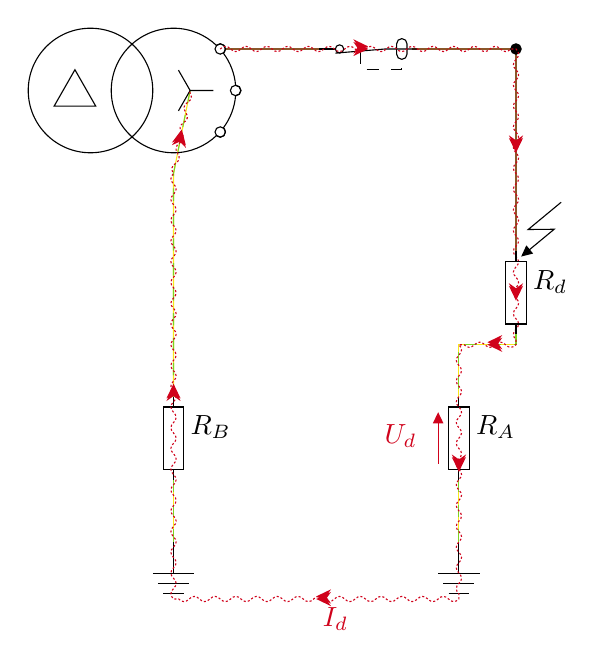
\begin{tikzpicture}[x=0.75pt,y=0.75pt,yscale=-1,xscale=1]
%uncomment if require: \path (0,353); %set diagram left start at 0, and has height of 353

%Straight Lines [id:da8450582290113836] 
\draw [color={rgb, 255:red, 248; green, 231; blue, 28 }  ,draw opacity=1 ]   (87.5,222.5) -- (87.5,252.5) ;
%Straight Lines [id:da035234150750507176] 
\draw [color={rgb, 255:red, 248; green, 231; blue, 28 }  ,draw opacity=1 ]   (252.5,152.5) -- (252.5,157.5) -- (225,157.5) -- (225,182.5) ;
%Straight Lines [id:da575921985906619] 
\draw [color={rgb, 255:red, 139; green, 87; blue, 42 }  ,draw opacity=1 ]   (112.5,15) -- (162.5,15) ;
%Straight Lines [id:da5726536295563455] 
\draw [color={rgb, 255:red, 248; green, 231; blue, 28 }  ,draw opacity=1 ]   (95.5,35) -- (87.5,75) -- (87.5,182.5) ;
%Straight Lines [id:da38476257001275427] 
\draw [color={rgb, 255:red, 126; green, 211; blue, 33 }  ,draw opacity=1 ] [dash pattern={on 4.5pt off 4.5pt}]  (95.5,35) -- (87.5,75) -- (87.5,182.5) ;
%Straight Lines [id:da9973940303994429] 
\draw [color={rgb, 255:red, 139; green, 87; blue, 42 }  ,draw opacity=1 ]   (202.5,15) -- (252.5,15) ;
%Shape: Path Data [id:dp9822778342813306] 
\draw   (112.5,55) .. controls (112.5,56.38) and (111.38,57.5) .. (110,57.5) .. controls (109.29,57.5) and (108.65,57.2) .. (108.19,56.72) .. controls (102.81,61.85) and (95.52,65) .. (87.5,65) .. controls (70.93,65) and (57.5,51.57) .. (57.5,35) .. controls (57.5,18.43) and (70.93,5) .. (87.5,5) .. controls (95.52,5) and (102.81,8.15) .. (108.19,13.28) .. controls (108.65,12.8) and (109.29,12.5) .. (110,12.5) .. controls (111.38,12.5) and (112.5,13.62) .. (112.5,15) .. controls (112.5,15.82) and (112.11,16.54) .. (111.5,17) .. controls (114.8,21.39) and (116.92,26.71) .. (117.4,32.5) .. controls (117.43,32.5) and (117.47,32.5) .. (117.5,32.5) .. controls (118.88,32.5) and (120,33.62) .. (120,35) .. controls (120,36.38) and (118.88,37.5) .. (117.5,37.5) .. controls (117.47,37.5) and (117.43,37.5) .. (117.4,37.5) .. controls (116.92,43.29) and (114.8,48.61) .. (111.5,53) .. controls (112.11,53.46) and (112.5,54.18) .. (112.5,55) -- cycle ;
%Shape: Circle [id:dp10169246549820965] 
\draw   (17.5,35) .. controls (17.5,18.43) and (30.93,5) .. (47.5,5) .. controls (64.07,5) and (77.5,18.43) .. (77.5,35) .. controls (77.5,51.57) and (64.07,65) .. (47.5,65) .. controls (30.93,65) and (17.5,51.57) .. (17.5,35) -- cycle ;
%Shape: Triangle [id:dp22185224755779764] 
\draw   (40,25) -- (30,42.5) -- (50,42.5) -- cycle ;
%Shape: Star [id:dp4535075510124722] 
\draw   (106.75,35) -- (95.5,35) -- (89.88,44.81) -- (95.5,35) -- (89.88,25.19) -- (95.5,35) -- cycle ;
%Shape: Circle [id:dp28187455970704567] 
\draw   (107.5,15) .. controls (107.5,13.62) and (108.62,12.5) .. (110,12.5) .. controls (111.38,12.5) and (112.5,13.62) .. (112.5,15) .. controls (112.5,16.38) and (111.38,17.5) .. (110,17.5) .. controls (108.62,17.5) and (107.5,16.38) .. (107.5,15) -- cycle ;
%Shape: Circle [id:dp9096244123377861] 
\draw   (114.9,35) .. controls (114.9,33.62) and (116.02,32.5) .. (117.4,32.5) .. controls (118.78,32.5) and (119.9,33.62) .. (119.9,35) .. controls (119.9,36.38) and (118.78,37.5) .. (117.4,37.5) .. controls (116.02,37.5) and (114.9,36.38) .. (114.9,35) -- cycle ;
%Shape: Circle [id:dp0660770114066822] 
\draw   (107.5,55) .. controls (107.5,53.62) and (108.62,52.5) .. (110,52.5) .. controls (111.38,52.5) and (112.5,53.62) .. (112.5,55) .. controls (112.5,56.38) and (111.38,57.5) .. (110,57.5) .. controls (108.62,57.5) and (107.5,56.38) .. (107.5,55) -- cycle ;

%Straight Lines [id:da12486709959480935] 
\draw [color={rgb, 255:red, 139; green, 87; blue, 42 }  ,draw opacity=1 ]   (252.5,112.5) -- (252.5,17.5) ;
%Straight Lines [id:da9194886303106931] 
\draw [color={rgb, 255:red, 126; green, 211; blue, 33 }  ,draw opacity=1 ] [dash pattern={on 4.5pt off 4.5pt}]  (252.5,152.5) -- (252.5,157.5) -- (225,157.5) -- (225,182.5) ;
%Straight Lines [id:da33889517147418446] 
\draw    (87.5,252.5) -- (87.5,267.5) ;
%Straight Lines [id:da7536356147270271] 
\draw    (77.5,267.5) -- (97.5,267.5) ;
%Straight Lines [id:da33790733335159795] 
\draw    (80,272.5) -- (95,272.5) ;
%Straight Lines [id:da8225336413065082] 
\draw    (82.5,277.5) -- (92.5,277.5) ;

%Straight Lines [id:da14728368722832463] 
\draw [color={rgb, 255:red, 126; green, 211; blue, 33 }  ,draw opacity=1 ] [dash pattern={on 4.5pt off 4.5pt}]  (87.5,222.5) -- (87.5,252.5) ;
%Straight Lines [id:da2713756434582886] 
\draw [color={rgb, 255:red, 248; green, 231; blue, 28 }  ,draw opacity=1 ]   (225,222.5) -- (225,252.5) ;
%Straight Lines [id:da07200185094723521] 
\draw    (225,252.5) -- (225,267.5) ;
%Straight Lines [id:da5503731135148442] 
\draw    (215,267.5) -- (235,267.5) ;
%Straight Lines [id:da9244125108161202] 
\draw    (217.5,272.5) -- (232.5,272.5) ;
%Straight Lines [id:da07512791048030887] 
\draw    (220,277.5) -- (230,277.5) ;

%Straight Lines [id:da5491926071123034] 
\draw [color={rgb, 255:red, 126; green, 211; blue, 33 }  ,draw opacity=1 ] [dash pattern={on 4.5pt off 4.5pt}]  (225,222.5) -- (225,252.5) ;
%Straight Lines [id:da7705666086878261] 
\draw    (87.5,217.5) -- (87.5,222.5) ;
%Shape: Rectangle [id:dp5724900932521552] 
\draw   (92.5,187.5) -- (92.5,217.5) -- (82.5,217.5) -- (82.5,187.5) -- cycle ;
%Straight Lines [id:da6857493814799358] 
\draw    (87.5,182.5) -- (87.5,187.5) ;

%Straight Lines [id:da7810225170823131] 
\draw    (225,217.5) -- (225,222.5) ;
%Shape: Rectangle [id:dp9839408028922504] 
\draw   (230,187.5) -- (230,217.5) -- (220,217.5) -- (220,187.5) -- cycle ;
%Straight Lines [id:da4367313473487816] 
\draw    (225,182.5) -- (225,187.5) ;

%Shape: Circle [id:dp6401617010113628] 
\draw  [fill={rgb, 255:red, 0; green, 0; blue, 0 }  ,fill opacity=1 ] (250,15) .. controls (250,13.62) and (251.12,12.5) .. (252.5,12.5) .. controls (253.88,12.5) and (255,13.62) .. (255,15) .. controls (255,16.38) and (253.88,17.5) .. (252.5,17.5) .. controls (251.12,17.5) and (250,16.38) .. (250,15) -- cycle ;
%Rounded Rect [id:dp9837999595449706] 
\draw   (197.5,20) .. controls (196.12,20) and (195,18.88) .. (195,17.5) -- (195,12.5) .. controls (195,11.12) and (196.12,10) .. (197.5,10) -- (197.5,10) .. controls (198.88,10) and (200,11.12) .. (200,12.5) -- (200,17.5) .. controls (200,18.88) and (198.88,20) .. (197.5,20) -- cycle ;
%Straight Lines [id:da04140906911364939] 
\draw  [dash pattern={on 4.5pt off 4.5pt}]  (177.5,16) -- (177.5,25) -- (197.5,25) -- (197.5,20) ;
%Shape: Circle [id:dp7012058816599942] 
\draw   (167.5,13) .. controls (166.4,13) and (165.5,13.9) .. (165.5,15) .. controls (165.5,16.1) and (166.4,17) .. (167.5,17) .. controls (168.6,17) and (169.5,16.1) .. (169.5,15) .. controls (169.5,13.9) and (168.6,13) .. (167.5,13) -- cycle ;
%Straight Lines [id:da23692932983683102] 
\draw    (165.5,15) -- (157.5,15) ;
%Straight Lines [id:da4567235518407359] 
\draw    (165.5,17) -- (189.5,15) -- (205,15) ;
%Shape: Boxed Line [id:dp44753967705251496] 
\draw    (274.27,88.83) -- (258.39,101.97) -- (270.89,101.86) -- (257.31,113.09) ;
\draw [shift={(255,115)}, rotate = 320.40999999999997] [fill={rgb, 255:red, 0; green, 0; blue, 0 }  ][line width=0.08]  [draw opacity=0] (5.36,-2.57) -- (0,0) -- (5.36,2.57) -- cycle    ;
\draw [color={rgb, 255:red, 208; green, 2; blue, 27 }  ,draw opacity=1 ] [dash pattern={on 0.75pt off 0.75pt}]  (110,15) .. controls (111.67,13.33) and (113.33,13.33) .. (115,15) .. controls (116.67,16.67) and (118.33,16.67) .. (120,15) .. controls (121.67,13.33) and (123.33,13.33) .. (125,15) .. controls (126.67,16.67) and (128.33,16.67) .. (130,15) .. controls (131.67,13.33) and (133.33,13.33) .. (135,15) .. controls (136.67,16.67) and (138.33,16.67) .. (140,15) .. controls (141.67,13.33) and (143.33,13.33) .. (145,15) .. controls (146.67,16.67) and (148.33,16.67) .. (150,15) .. controls (151.67,13.33) and (153.33,13.33) .. (155,15) .. controls (156.67,16.67) and (158.33,16.67) .. (160,15) .. controls (161.67,13.33) and (163.33,13.33) .. (165,15) .. controls (166.67,16.67) and (168.33,16.67) .. (170,15) .. controls (171.67,13.33) and (173.33,13.33) .. (175,15) .. controls (176.67,16.67) and (178.33,16.67) .. (180,15) .. controls (181.67,13.33) and (183.33,13.33) .. (185,15) .. controls (186.67,16.67) and (188.33,16.67) .. (190,15) .. controls (191.67,13.33) and (193.33,13.33) .. (195,15) .. controls (196.67,16.67) and (198.33,16.67) .. (200,15) .. controls (201.67,13.33) and (203.33,13.33) .. (205,15) .. controls (206.67,16.67) and (208.33,16.67) .. (210,15) .. controls (211.67,13.33) and (213.33,13.33) .. (215,15) .. controls (216.67,16.67) and (218.33,16.67) .. (220,15) .. controls (221.67,13.33) and (223.33,13.33) .. (225,15) .. controls (226.67,16.67) and (228.33,16.67) .. (230,15) .. controls (231.67,13.33) and (233.33,13.33) .. (235,15) .. controls (236.67,16.67) and (238.33,16.67) .. (240,15) .. controls (241.67,13.33) and (243.33,13.33) .. (245,15) .. controls (246.67,16.67) and (248.33,16.67) .. (250,15) -- (252.5,15) -- (252.5,15) .. controls (254.17,16.67) and (254.17,18.33) .. (252.5,20) .. controls (250.83,21.67) and (250.83,23.33) .. (252.5,25) .. controls (254.17,26.67) and (254.17,28.33) .. (252.5,30) .. controls (250.83,31.67) and (250.83,33.33) .. (252.5,35) .. controls (254.17,36.67) and (254.17,38.33) .. (252.5,40) .. controls (250.83,41.67) and (250.83,43.33) .. (252.5,45) .. controls (254.17,46.67) and (254.17,48.33) .. (252.5,50) .. controls (250.83,51.67) and (250.83,53.33) .. (252.5,55) .. controls (254.17,56.67) and (254.17,58.33) .. (252.5,60) .. controls (250.83,61.67) and (250.83,63.33) .. (252.5,65) .. controls (254.17,66.67) and (254.17,68.33) .. (252.5,70) .. controls (250.83,71.67) and (250.83,73.33) .. (252.5,75) .. controls (254.17,76.67) and (254.17,78.33) .. (252.5,80) .. controls (250.83,81.67) and (250.83,83.33) .. (252.5,85) .. controls (254.17,86.67) and (254.17,88.33) .. (252.5,90) .. controls (250.83,91.67) and (250.83,93.33) .. (252.5,95) .. controls (254.17,96.67) and (254.17,98.33) .. (252.5,100) .. controls (250.83,101.67) and (250.83,103.33) .. (252.5,105) .. controls (254.17,106.67) and (254.17,108.33) .. (252.5,110) .. controls (250.83,111.67) and (250.83,113.33) .. (252.5,115) -- (252.5,115) .. controls (254.17,116.67) and (254.17,118.33) .. (252.5,120) .. controls (250.83,121.67) and (250.83,123.33) .. (252.5,125) .. controls (254.17,126.67) and (254.17,128.33) .. (252.5,130) .. controls (250.83,131.67) and (250.83,133.33) .. (252.5,135) .. controls (254.17,136.67) and (254.17,138.33) .. (252.5,140) .. controls (250.83,141.67) and (250.83,143.33) .. (252.5,145) .. controls (254.17,146.67) and (254.17,148.33) .. (252.5,150) .. controls (250.83,151.67) and (250.83,153.33) .. (252.5,155) -- (252.5,157.5) -- (252.5,157.5) .. controls (250.83,159.17) and (249.17,159.17) .. (247.5,157.5) .. controls (245.83,155.83) and (244.17,155.83) .. (242.5,157.5) .. controls (240.83,159.17) and (239.17,159.17) .. (237.5,157.5) .. controls (235.83,155.83) and (234.17,155.83) .. (232.5,157.5) .. controls (230.83,159.17) and (229.17,159.17) .. (227.5,157.5) -- (225,157.5) -- (225,157.5) .. controls (226.67,159.17) and (226.67,160.83) .. (225,162.5) .. controls (223.33,164.17) and (223.33,165.83) .. (225,167.5) .. controls (226.67,169.17) and (226.67,170.83) .. (225,172.5) .. controls (223.33,174.17) and (223.33,175.83) .. (225,177.5) .. controls (226.67,179.17) and (226.67,180.83) .. (225,182.5) .. controls (223.33,184.17) and (223.33,185.83) .. (225,187.5) .. controls (226.67,189.17) and (226.67,190.83) .. (225,192.5) .. controls (223.33,194.17) and (223.33,195.83) .. (225,197.5) .. controls (226.67,199.17) and (226.67,200.83) .. (225,202.5) .. controls (223.33,204.17) and (223.33,205.83) .. (225,207.5) .. controls (226.67,209.17) and (226.67,210.83) .. (225,212.5) .. controls (223.33,214.17) and (223.33,215.83) .. (225,217.5) .. controls (226.67,219.17) and (226.67,220.83) .. (225,222.5) .. controls (223.33,224.17) and (223.33,225.83) .. (225,227.5) .. controls (226.67,229.17) and (226.67,230.83) .. (225,232.5) .. controls (223.33,234.17) and (223.33,235.83) .. (225,237.5) .. controls (226.67,239.17) and (226.67,240.83) .. (225,242.5) .. controls (223.33,244.17) and (223.33,245.83) .. (225,247.5) .. controls (226.67,249.17) and (226.67,250.83) .. (225,252.5) .. controls (223.33,254.17) and (223.33,255.83) .. (225,257.5) .. controls (226.67,259.17) and (226.67,260.83) .. (225,262.5) .. controls (223.33,264.17) and (223.33,265.83) .. (225,267.5) .. controls (226.67,269.17) and (226.67,270.83) .. (225,272.5) .. controls (223.33,274.17) and (223.33,275.83) .. (225,277.5) -- (225,280) -- (225,280) .. controls (223.33,281.67) and (221.67,281.67) .. (220,280) .. controls (218.33,278.33) and (216.67,278.33) .. (215,280) .. controls (213.33,281.67) and (211.67,281.67) .. (210,280) .. controls (208.33,278.33) and (206.67,278.33) .. (205,280) .. controls (203.33,281.67) and (201.67,281.67) .. (200,280) .. controls (198.33,278.33) and (196.67,278.33) .. (195,280) .. controls (193.33,281.67) and (191.67,281.67) .. (190,280) .. controls (188.33,278.33) and (186.67,278.33) .. (185,280) .. controls (183.33,281.67) and (181.67,281.67) .. (180,280) .. controls (178.33,278.33) and (176.67,278.33) .. (175,280) .. controls (173.33,281.67) and (171.67,281.67) .. (170,280) .. controls (168.33,278.33) and (166.67,278.33) .. (165,280) .. controls (163.33,281.67) and (161.67,281.67) .. (160,280) .. controls (158.33,278.33) and (156.67,278.33) .. (155,280) .. controls (153.33,281.67) and (151.67,281.67) .. (150,280) .. controls (148.33,278.33) and (146.67,278.33) .. (145,280) .. controls (143.33,281.67) and (141.67,281.67) .. (140,280) .. controls (138.33,278.33) and (136.67,278.33) .. (135,280) .. controls (133.33,281.67) and (131.67,281.67) .. (130,280) .. controls (128.33,278.33) and (126.67,278.33) .. (125,280) .. controls (123.33,281.67) and (121.67,281.67) .. (120,280) .. controls (118.33,278.33) and (116.67,278.33) .. (115,280) .. controls (113.33,281.67) and (111.67,281.67) .. (110,280) .. controls (108.33,278.33) and (106.67,278.33) .. (105,280) .. controls (103.33,281.67) and (101.67,281.67) .. (100,280) .. controls (98.33,278.33) and (96.67,278.33) .. (95,280) .. controls (93.33,281.67) and (91.67,281.67) .. (90,280) -- (87.5,280) -- (87.5,280) .. controls (85.83,278.33) and (85.83,276.67) .. (87.5,275) .. controls (89.17,273.33) and (89.17,271.67) .. (87.5,270) .. controls (85.83,268.33) and (85.83,266.67) .. (87.5,265) .. controls (89.17,263.33) and (89.17,261.67) .. (87.5,260) .. controls (85.83,258.33) and (85.83,256.67) .. (87.5,255) .. controls (89.17,253.33) and (89.17,251.67) .. (87.5,250) .. controls (85.83,248.33) and (85.83,246.67) .. (87.5,245) .. controls (89.17,243.33) and (89.17,241.67) .. (87.5,240) .. controls (85.83,238.33) and (85.83,236.67) .. (87.5,235) .. controls (89.17,233.33) and (89.17,231.67) .. (87.5,230) .. controls (85.83,228.33) and (85.83,226.67) .. (87.5,225) .. controls (89.17,223.33) and (89.17,221.67) .. (87.5,220) .. controls (85.83,218.33) and (85.83,216.67) .. (87.5,215) .. controls (89.17,213.33) and (89.17,211.67) .. (87.5,210) .. controls (85.83,208.33) and (85.83,206.67) .. (87.5,205) .. controls (89.17,203.33) and (89.17,201.67) .. (87.5,200) .. controls (85.83,198.33) and (85.83,196.67) .. (87.5,195) .. controls (89.17,193.33) and (89.17,191.67) .. (87.5,190) .. controls (85.83,188.33) and (85.83,186.67) .. (87.5,185) .. controls (89.17,183.33) and (89.17,181.67) .. (87.5,180) .. controls (85.83,178.33) and (85.83,176.67) .. (87.5,175) .. controls (89.17,173.33) and (89.17,171.67) .. (87.5,170) .. controls (85.83,168.33) and (85.83,166.67) .. (87.5,165) .. controls (89.17,163.33) and (89.17,161.67) .. (87.5,160) .. controls (85.83,158.33) and (85.83,156.67) .. (87.5,155) .. controls (89.17,153.33) and (89.17,151.67) .. (87.5,150) .. controls (85.83,148.33) and (85.83,146.67) .. (87.5,145) .. controls (89.17,143.33) and (89.17,141.67) .. (87.5,140) .. controls (85.83,138.33) and (85.83,136.67) .. (87.5,135) .. controls (89.17,133.33) and (89.17,131.67) .. (87.5,130) .. controls (85.83,128.33) and (85.83,126.67) .. (87.5,125) .. controls (89.17,123.33) and (89.17,121.67) .. (87.5,120) .. controls (85.83,118.33) and (85.83,116.67) .. (87.5,115) .. controls (89.17,113.33) and (89.17,111.67) .. (87.5,110) .. controls (85.83,108.33) and (85.83,106.67) .. (87.5,105) .. controls (89.17,103.33) and (89.17,101.67) .. (87.5,100) .. controls (85.83,98.33) and (85.83,96.67) .. (87.5,95) .. controls (89.17,93.33) and (89.17,91.67) .. (87.5,90) .. controls (85.83,88.33) and (85.83,86.67) .. (87.5,85) .. controls (89.17,83.33) and (89.17,81.67) .. (87.5,80) .. controls (85.83,78.33) and (85.83,76.67) .. (87.5,75) -- (87.5,75) .. controls (86.19,73.04) and (86.52,71.41) .. (88.48,70.1) .. controls (90.44,68.79) and (90.77,67.15) .. (89.46,65.19) .. controls (88.15,63.23) and (88.48,61.6) .. (90.44,60.29) .. controls (92.4,58.98) and (92.73,57.35) .. (91.42,55.39) .. controls (90.11,53.43) and (90.44,51.8) .. (92.4,50.49) .. controls (94.36,49.18) and (94.69,47.54) .. (93.38,45.58) .. controls (92.07,43.62) and (92.4,41.99) .. (94.36,40.68) .. controls (96.32,39.37) and (96.65,37.74) .. (95.34,35.78) -- (95.5,35) -- (95.5,35) ;
\draw [shift={(181.25,15)}, rotate = 180] [fill={rgb, 255:red, 208; green, 2; blue, 27 }  ,fill opacity=1 ][line width=0.08]  [draw opacity=0] (7.14,-3.43) -- (0,0) -- (7.14,3.43) -- (4.74,0) -- cycle    ;
\draw [shift={(252.5,65)}, rotate = 270] [fill={rgb, 255:red, 208; green, 2; blue, 27 }  ,fill opacity=1 ][line width=0.08]  [draw opacity=0] (7.14,-3.43) -- (0,0) -- (7.14,3.43) -- (4.74,0) -- cycle    ;
\draw [shift={(252.5,136.25)}, rotate = 270] [fill={rgb, 255:red, 208; green, 2; blue, 27 }  ,fill opacity=1 ][line width=0.08]  [draw opacity=0] (7.14,-3.43) -- (0,0) -- (7.14,3.43) -- (4.74,0) -- cycle    ;
\draw [shift={(238.75,157.5)}, rotate = 360] [fill={rgb, 255:red, 208; green, 2; blue, 27 }  ,fill opacity=1 ][line width=0.08]  [draw opacity=0] (7.14,-3.43) -- (0,0) -- (7.14,3.43) -- (4.74,0) -- cycle    ;
\draw [shift={(225,218.75)}, rotate = 270] [fill={rgb, 255:red, 208; green, 2; blue, 27 }  ,fill opacity=1 ][line width=0.08]  [draw opacity=0] (7.14,-3.43) -- (0,0) -- (7.14,3.43) -- (4.74,0) -- cycle    ;
\draw [shift={(156.25,280)}, rotate = 360] [fill={rgb, 255:red, 208; green, 2; blue, 27 }  ,fill opacity=1 ][line width=0.08]  [draw opacity=0] (7.14,-3.43) -- (0,0) -- (7.14,3.43) -- (4.74,0) -- cycle    ;
\draw [shift={(87.5,177.5)}, rotate = 450] [fill={rgb, 255:red, 208; green, 2; blue, 27 }  ,fill opacity=1 ][line width=0.08]  [draw opacity=0] (7.14,-3.43) -- (0,0) -- (7.14,3.43) -- (4.74,0) -- cycle    ;
\draw [shift={(91.5,55)}, rotate = 461.31] [fill={rgb, 255:red, 208; green, 2; blue, 27 }  ,fill opacity=1 ][line width=0.08]  [draw opacity=0] (7.14,-3.43) -- (0,0) -- (7.14,3.43) -- (4.74,0) -- cycle    ;
\draw [shift={(181.25,13.75)}, rotate = 180] [fill={rgb, 255:red, 208; green, 2; blue, 27 }  ,fill opacity=1 ][line width=0.08]  [draw opacity=0] (7.14,-3.43) -- (0,0) -- (7.14,3.43) -- (4.74,0) -- cycle    ;
\draw [shift={(252.5,63.75)}, rotate = 270] [fill={rgb, 255:red, 208; green, 2; blue, 27 }  ,fill opacity=1 ][line width=0.08]  [draw opacity=0] (7.14,-3.43) -- (0,0) -- (7.14,3.43) -- (4.74,0) -- cycle    ;
\draw [shift={(252.5,135)}, rotate = 270] [fill={rgb, 255:red, 208; green, 2; blue, 27 }  ,fill opacity=1 ][line width=0.08]  [draw opacity=0] (7.14,-3.43) -- (0,0) -- (7.14,3.43) -- (4.74,0) -- cycle    ;
\draw [shift={(238.75,156.25)}, rotate = 360] [fill={rgb, 255:red, 208; green, 2; blue, 27 }  ,fill opacity=1 ][line width=0.08]  [draw opacity=0] (7.14,-3.43) -- (0,0) -- (7.14,3.43) -- (4.74,0) -- cycle    ;
\draw [shift={(225,217.5)}, rotate = 270] [fill={rgb, 255:red, 208; green, 2; blue, 27 }  ,fill opacity=1 ][line width=0.08]  [draw opacity=0] (7.14,-3.43) -- (0,0) -- (7.14,3.43) -- (4.74,0) -- cycle    ;
\draw [shift={(156.25,278.75)}, rotate = 360] [fill={rgb, 255:red, 208; green, 2; blue, 27 }  ,fill opacity=1 ][line width=0.08]  [draw opacity=0] (7.14,-3.43) -- (0,0) -- (7.14,3.43) -- (4.74,0) -- cycle    ;
\draw [shift={(87.5,176.25)}, rotate = 450] [fill={rgb, 255:red, 208; green, 2; blue, 27 }  ,fill opacity=1 ][line width=0.08]  [draw opacity=0] (7.14,-3.43) -- (0,0) -- (7.14,3.43) -- (4.74,0) -- cycle    ;
\draw [shift={(91.5,53.75)}, rotate = 461.31] [fill={rgb, 255:red, 208; green, 2; blue, 27 }  ,fill opacity=1 ][line width=0.08]  [draw opacity=0] (7.14,-3.43) -- (0,0) -- (7.14,3.43) -- (4.74,0) -- cycle    ;
%Straight Lines [id:da9207949526828273] 
\draw    (252.5,147.5) -- (252.5,152.5) ;
%Shape: Rectangle [id:dp36210266951689685] 
\draw   (257.5,117.5) -- (257.5,147.5) -- (247.5,147.5) -- (247.5,117.5) -- cycle ;
%Straight Lines [id:da2843419817195654] 
\draw    (252.5,112.5) -- (252.5,117.5) ;

%Straight Lines [id:da667113945803525] 
\draw [color={rgb, 255:red, 208; green, 2; blue, 27 }  ,draw opacity=1 ]   (215,193) -- (215,215) ;
\draw [shift={(215,190)}, rotate = 90] [fill={rgb, 255:red, 208; green, 2; blue, 27 }  ,fill opacity=1 ][line width=0.08]  [draw opacity=0] (5.36,-2.57) -- (0,0) -- (5.36,2.57) -- cycle    ;

% Text Node
\draw (94.5,190.5) node [anchor=north west][inner sep=0.75pt]   [align=left] {$R_B$};
% Text Node
\draw (232,190.5) node [anchor=north west][inner sep=0.75pt]   [align=left] {$R_A$};
% Text Node
\draw (188,194.5) node [anchor=north west][inner sep=0.75pt]  [color={rgb, 255:red, 208; green, 2; blue, 27 }  ,opacity=1 ] [align=left] {$U_d$};
% Text Node
\draw (259.5,120.5) node [anchor=north west][inner sep=0.75pt]   [align=left] {$R_d$};
% Text Node
\draw (158.25,283) node [anchor=north west][inner sep=0.75pt] [color={rgb, 255:red, 208; green, 2; blue, 27 }]  [align=left] {$I_d$};


\end{tikzpicture}

\end{figure}

%\end{document}


\begin{comment}
\begin{circuitikz}[circuit ee IEC relay]
%\DrawGrid{(-1,-5)}{(9,3)} %grille d'aide pour le placement des objets

%alimentation

\node (D1) [make contact=point left, circuit breaker={point left}, tiny circuit symbols, activated] at (1,0.45) {};
\node (T1) [oosourcetransshape, prim=delta,sec=wye] at (0,0) {};


%neutre/terre

\node (RN) [R, label=$R_B$, rotate=90, tiny circuit symbols] at (0,-2.7) {};
\node (G1) [tlground] at (0,-3.9) {};
\draw [green!, thick] (G1) to node {} (RN) ; 
\draw [green!, thick] (RN) to (0,-0.5) to node {} (T1.sec4) ; 
\draw [dashed, yellow!, thick] (G1) to node {} (RN) ;
\draw [dashed, yellow!, thick] (RN) to (0,-0.5) to node {} (T1.sec4) ;

\node (RT) [resistor, rotate=90, tiny circuit symbols, label=$R_A$] at (2.5,-2.7) {};
\draw[-triangle 45, red] (2.8,-2) -- (2.8,-1) node[right,midway] {$U_d$};
\node (G2) [tlground] at (2.5,-3.9) {};
\draw [green!, thick] (RT) to (G2); 
\draw [dashed, yellow!, thick] (RT) to (G2);
\node (G2) [tlground] at (2.5,-3.9) {};
\draw [green!, thick] (G1) to (0,-4.2) to (2.5,-4.2) to (G2);
\draw [dashed, yellow!, thick] (G1) -- (0,-4.2) -- (2.5,-4.2) node [midway,below] {\color{black}$I_d$} -- (G2);
\node (G1) [tlground] at (0,-3.9) {};
\node (G2) [tlground] at (2.5,-3.9) {};

%appareil 1

\node (C2) [circ, scale=0.5] at (2.5,0.45) {};
\node (RD) [resistor, label=$R_d$, rotate=90, tiny circuit symbols] at (2.5,-1.5) {};

\draw [green!, thick] (RD) to (RT); 
\draw [dashed, yellow!, thick] (RD) to (RT); 

\draw [brown, thick] (T1.sec1) to (0.5,0.45) to (D1) to (C2) to (RD);
\node (T1) [oosourcetransshape, prim=delta,sec=wye] at (0,0) {};

%chemin courant

\fill [yellow!, decoration=lightning bolt, decorate] (2.5,-1.2) -- ++ (0.5,0.8); %éclairs
\path [postaction={on each segment={mid arrow=red}}]  (T1.sec1) -- (0.5,0.45) -- (D1) -- (C2) -- (RD) -- (RT) -- (G2) -- (2.5,-4.2) -- (1.666,-4.2) -- (0.88888,-4.2)  -- (0,-4.2) -- (G1) -- (RN) -- (0,-0.5) -- (T1.sec4); 

\callout{1,-0.5}{\cstep\label{pas:1}}{2.4,-1.2};


\end{circuitikz}
\end{comment}


L'intensité de courant $I_d$ vaut alors :
\begin{formule}[Courant de défaut $I_d$ en schéma TT]
\begin{align*}
		I_d &= \frac{U_{0}}{R_{B}+R_{A}+R_{d}}
\end{align*}
\end{formule}

\begin{textvariables}
U_{0}						& tension nominale simple						& volt			& \volt					& 	Différence de potentiel entre les masses métalliques et la terre 	\\
R_{B}						& résistance						& ohm			& \ohm					& 	Résistance de la prise de terre du neutre 	\\
R_{A}						& résistance						& ohm			& \ohm					& 	Résistance de la prise de terre de l'installation électrique 	\\
R_{d}						& résistance						& ohm			& \ohm					& 	Résistance de défaut 	d'isolement \\
\end{textvariables}

Le courant de défaut $I_d$ fera alors apparaître une \emph{tension de défaut} $U_d$ entre la masse métallique et la terre. Pour satisfaire aux normes de sécurité de la NF C15-100, il est imposé que la tension de défaut $U_d$ ne dépasse pas la tension de sécurité du local $U_L$ (voir \superref{subsec:prise_terre_installation_electrique}) :

\begin{formule}[Tension de défaut $U_d$ en schéma TT]
\begin{align*}
		U_d &= R_{A} \times I_{d} \\
			   &< U_L
\end{align*}
\end{formule}

\begin{textvariables}
R_{A}						& résistance						& ohm			& \ohm					& 	Résistance de la prise de terre de l'installation électrique 	\\
I_{d}							& intensité							& ampère		& \ampere				& 	Courant de défaut d'isolement \\
U_{L}						& tension							& volt			& \volt					& 	Tension de sécurité du local avec :
\begin{description}[nosep, leftmargin=*]
\item[Local sec :] $U_{L}=\SI{50}{\volt}$
\item[Local humide :] $U_{L}=\SI{25}{\volt}$
\end{description} \\
\end{textvariables}

Il est donc nécessaire de limiter $U_d$ à la valeur suivante (voir \superref{form:resistance_prise_terre}) :

\begin{formule}[Calibre du DDR $I_{\Delta n}$]
\begin{align*}
		I_{\Delta n} &< \frac{U_{L}}{R_{A}}
\end{align*}
\end{formule}

\begin{textvariables}
U_{L}						& tension							& volt			& \volt					& 	Tension de sécurité du local avec :
\begin{description}[nosep, leftmargin=*]
\item[Local sec :] $U_{L}=\SI{50}{\volt}$
\item[Local humide :] $U_{L}=\SI{25}{\volt}$
\end{description} \\
R_{A}						& résistance						& ohm			& \ohm					& 	Résistance de la prise de terre de l'installation électrique 	\\
\end{textvariables}

\begin{exemple}[Calcul du calibre du DDR $I_{\Delta n}$]
Si on considère que le transformateur est un transformateur $\SI{20}{\kilo\volt}/\SI{400}{\volt}$, que $R_A=\SI{20}{\ohm}$, que $R_B=\SI{10}{\ohm}$ et que $R_d$ est négligée, on peut déduire que le courant de défaut $I_d$ vaut :
\begin{align*}
		I_d 	&= \frac{U_{0}}{R_{B}+R_{A}} \\
				&=\frac{400}{20+10} \\
				&= \SI{13,33}{\ampere} \\
\end{align*}
Si une personne touche une masse des récepteurs en défaut, elle sera soumise à une tension de défaut $U_d$ :
\begin{align*}
		U_d 	&= R_{A} \times I_{d} \\
				&=20 \times 13,33 \\
				&= \SI{266,6}{\volt}
\end{align*}
La tension de défaut $U_d$ est dangereuse quelle que soit la tension limite choisie :
\begin{itemize}
\item coupure la plus rapide possible\,;
\item protection des personnes.
\end{itemize}
~\\
\begin{minipage}[t]{0.5\linewidth}
Dans le cas d'un local sec :
\begin{align*}
	I_{\Delta n} 	&< \frac{U_{L}}{R_{A}} \\
						&< \frac{50}{20} \\
						&< \SI{2,5}{\ampere}
\end{align*}
\end{minipage}
\hfill
\begin{minipage}[t]{0.5\linewidth}
Dans le cas d'un local humide :
\begin{align*}
	I_{\Delta n} 	&< \frac{U_{L}}{R_{A}} \\
						&< \frac{25}{20} \\
						&< \SI{1,25}{\ampere}
\end{align*}
\end{minipage}
~\\
D'après le tableau situé en \superref{tab:temps_coupure_DDR}, le DDR doit présenter un temps de coupure de moins de \SI{70}{\milli\second} avec une tension de défaut $U_d$ de \SI{266,6}{\volt} :

\begin{table}[h]
\begin{tabularx}{\linewidth}{X cccccccc}
\toprule
Tension nominale		& \multicolumn{2}{c}{$\SI{50}{\volt}<U_0\leq\SI{120}{\volt}$} 	& \multicolumn{2}{c}{$\SI{120}{\volt}<U_0\leq\SI{230}{\volt}$} & \multicolumn{2}{c}{$\SI{230}{\volt}<U_0\leq\SI{400}{\volt}$}		& \multicolumn{2}{c}{$U_0>\SI{400}{\volt}$}\\
\midrule
Type de courant		& alternatif	& continu	& alternatif	& continu	& alternatif	& continu	& alternatif	& continu \\
\addlinespace
Schéma TN/IT	& \SI{0,8}{\second}	&	\SI{5}{\second}	&	\SI{0,4}{\second}	&	\SI{5}{\second}	&	\SI{0,2}{\second}	&	\SI{0,4}{\second}	&	\SI{0,1}{\second}	&	\SI{0,1}{\second} \\	
\addlinespace
Schéma TT	& \SI{0,3}{\second}	&	\SI{5}{\second}	&	\SI{0,2}{\second}	&	\SI{0,4}{\second}	&	\cellcolor{green}\SI{0,07}{\second}	&	\SI{0,2}{\second}	&	\SI{0,04}{\second}	&	\SI{0,1}{\second} \\	
\bottomrule
\end{tabularx}
\end{table}
\end{exemple}

%\end{document}


	%--------------------------------------
	%style des annexes
	%--------------------------------------
	
	\Framefalse %défini la booléenne Frame comme false -> pas de marqueurs de chapitre
	\appendix %appel des annexes
	\appendixpage

	%--------------------------------------
	%inclusion des chapitres
	%--------------------------------------

	%--------------------------------------
%ELECTROTECHNIQUE - SCHEMA DE LIAISON A LA TERRE
%--------------------------------------

%utiliser les environnement \begin{comment} \end{comment} pour mettre en commentaire le préambule une fois la programmation appelée dans le document maître (!ne pas oublier de mettre en commentaire \end{document}!)

\begin{comment}

\documentclass[a4paper, 11pt, twoside, fleqn]{memoir}

\usepackage{AOCDTF}

\input{marqueur_chapitre_couleur} %à personnaliser selon le nombre de chapitre dans le cours

%--------------------------------------
%corps du document
%--------------------------------------

\begin{document} %corps du document
	\openleft %début de chapitre à gauche

\end{comment}

\chapter{Informations complémentaires sur les dangers de l'électricité}

Cette annexe regroupe des données complémentaires mentionnées dans le \superref{chap:dangers_electricite}. Il n'est pas nécessaire de les retenir par c\oe{}ur mais ces informations constituent un support appréciable pour toute précision concernant ce chapitre.

\section{\'Etat des lieux de la prévention des risques électriques\label{sec:etat_lieux_prevention_electrique}}

\section{Statistiques}

\subsection{Accidents d'origine électrique}

Les accidents du travail d'origine électrique diminuent depuis la mise en place du décret du 14 novembre 1962 qui attrait à la protection des travailleurs contre les dangers de l'électricité. Entre 1962 et 2000, le nombre d'incidents a baissé de 74\%. 

\begin{center}
\begin{tikzpicture}
\begin{axis}[
/pgf/number format/.cd, use comma, 1000 sep={\,}, %format numérique européen
date coordinates in=x,
axis x line=bottom, axis y line = left,
xmin=1975-01-01,
xmax=2005-12-31,
ymin=0,
ymax=3100,
legend cell align={left},
no markers,
grid=major,
ytick={0, 500, 1000, 1500, 2000, 2500, 3000},
xtick={1975-01-01, 1980-01-01, 1985-01-01, 1990-01-01, 1995-01-01, 2000-01-01, 2005-01-01},
title={Variation du nombre d'accidents du travail d'origine électrique},
height=8cm,width=\linewidth,
ylabel={Nombre d'accidents},
legend entries={Accidents avec arrêt, Accidents graves, Accidents mortels},
xticklabel={\year},
]

\addplot[mark=none]table{donnees_accident_arret.txt};
\addlegendentry{Accidents avec arrêt};
\addplot[mark=none, red]table{donnees_accident_grave.txt};
\addlegendentry{Accidents graves};
\addplot[mark=none, blue]table{donnees_accident_mortel.txt};
\addlegendentry{Accidents mortels};
\end{axis}
\end{tikzpicture}
\end{center}

\subsection{Secteurs les plus atteints}

Durant l'année 2008, on dénombrait 771 accidents d'origine électrique. Les secteurs les plus touchés sont : 
\begin{description}
\item[30\% :] bâtiment et travaux publics,\;
\item[17\% :] métallurgie,\;
\item[16\% :] service et travail temporaire,\;
\item[11\% :] alimentation.
\end{description}

\subsection{Facteurs principaux}

Les principaux facteurs ayant causé l'accident sont :
\begin{description}
\item[31\% :] mode opératoire inapproprié ou dangereux\,;
\item[15\% :] application incomplète\,;
\item[12\% :] formation insuffisante\,;
\item[12\% :] état du matériel\,;
\item[11\% :] état du sol.
\end{description}

\subsection{Type de contact}

\begin{description}
\item[75\% :] contact direct\,;
\item[20\% :] contact indirect\,;
\item[5\% :] non précisé.
\end{description}

\subsection{Type de dommages}

Ces statistiques sur plusieurs années sont relativement constantes. Elles précisent que :
\begin{description}
\item[60\% :] brûlures\,;
\item[$\approx$ 33\% :] localisation multiples (les yeux, les membres supérieurs et les mains sont les plus touchés)\,;
\item[5\% :] lésions internes.
\end{description}

\subsection{Conclusion}

On peut conclure de ces statistiques que depuis une trentaine d'années, le nombre d'accidents dus à l'électricité :
\begin{itemize}
\item diminue régulièrement\,;
\item demeurent particulièrement graves.
\end{itemize}

Le risque d'accidents est certe mieux maitrisé qu'auparavant mais il reste toujours présent.

\section{Différents effets du courant électriques\label{sec:effet_courant_électrique}}

\subsection{Effet thermique}

Il est admis que les brûlures électriques peuvent apparaitre à des intensités relativement faibles ($\approx \SI{10}{\milli\ampere}$), si le contact est maintenu quelques minutes

\subsection{Effet tétanisant}

Lorsque la tension est alternatif, les muscles se situant sur le trajet du courant électrique se contractent. Cet effet, surtout s'il s'agit des muscles de la main, peuvent empêcher tout dégagement volontaire de la victime. Pour l'extraire de cette situation, il convient de stopper le contact crispé en la poussant à l'aide d'un objet non conducteur.

\subsection{Effets respiratoires et circulatoires}

Les muscles respiratoires pouvant également être crispés par le courant, il suffit de \SI{60}{\second} pour bloquer la respiration. Cela provoque une asphyxie, appelée également \emph{syncope blanche}.\\
Une fibrillation ventriculaire se manifeste également pour les mêmes ordres de grandeurs. C'est le résultat de la contraction anarchiques des fibrilles du muscle cardiaque. Ces battements du c\oe{}ur rapides et désordonnés ne permettent plus d'assurer une circulation sanguine adéquate et provoque ainsi une syncope cardiaque, appelée aussi \emph{syncope blanche}. Une défibrillation devient indispensable pour stopper cet effet du courant.\\
Au-delà d'un \SI{1}{\ampere}, le courant entraîne un arrêt cardiaque par asystolie, une absence de battements cardiaques sur laquelle une défibrillation n'est pas recommandée.\\
Les lésions cardiaques diffèrent selon certain paramètres, ces information peuvent aider les premiers secours à axer leurs interventions en situation d'extrême urgence : 
\begin{description}
\item[basse tension :] effet excito-moteur et fibrillation ventriculaire\,;
\item[haute tension :] effet joule et asystolie\,;
\item[foudre :] sidération myocardique (dysfonction des contractions du c\oe{}ur difficilement prise en charge).
\end{description}

Lors de la prise en charge d'un patient électrisé, il convient de bien suivre celui-ci sur plusieurs jours car les risques de malaises cardiaques dûs au choc électrique peuvent ressurgir durant une période plus ou moins longue selon les conditions d'électrisation.

\section{Descriptifs des moyens de protections contre les contacts directs}

Les différents moyens de protections sont ici décrits en profondeur à titre informatif.

\subsection{Très basse tension\label{subsec:TBT}}

Il existe trois types de TBT selon la classification du lieux et la nature du courant.

\subsubsection{Principe}

\paragraph{Très Basse Tension de Sécurité (ou Séparation)} Alimentation basse tension ou il n'existe aucun point commun entre le primaire et le secondaire du transformateur, utilisée pour alimenter des appareillages situés dans des locaux humides.
\paragraph{Très Basse Tension de Protection} Alimentation basse tension ou il existe un point commun entre le commun du secondaire et le conducteur de protection, utilisée pour alimenter des machines-outils et automatisme. La liaison du commun au conducteur de protection du secondaire permet d'éviter les mises en marche intempestives pouvant survenir après deux défauts de masse consécutifs dans une commande de machine (alimentation possible d'une bobine de contacteur via la carcasse de l'armoire de commande).
\paragraph{Très Basse Tension Fonctionnelle} Alimentation basse tension ou il existe plusieurs point commun entre le primaire et le secondaire du transformateur (autotransformateur), utilisée pour alimenter des appareillages ne requérant pas d'exigences de sécurité autre qu'une tension nominale de fonctionnement spécifique.

\subsubsection{Architecture}
%--------------------------------------
%ELECTROTECHNIQUE - SCHEMA DE LIAISON A LA TERRE
%--------------------------------------

%utiliser les environnement \begin{comment} \end{comment} pour mettre en commentaire le préambule une fois la programmation appelée dans le document maître (!ne pas oublier de mettre en commentaire \end{document}!)

\begin{comment}

\documentclass[a4paper, 11pt, twoside, fleqn]{memoir}

\usepackage{AOCDTF}
\marqueurchapitre

%lien d'édition des figures Tikz sur le site mathcha.io (rajouter le lien d'une modification effectuée sur la figure tikz avec le nom du modificateur car il n'y a qu'un lien par compte)

%lien éditeur Bruno Douchy : https://www.mathcha.io/editor/PkXjYIWPU5OtjyMlvDcpQ8KDDcwQoem6fnKOgwN

%--------------------------------------
%corps du document
%--------------------------------------

\begin{document} %corps du document
	\openleft %début de chapitre à gauche

\end{comment}

\begin{landscape}
\begin{table}
\caption{Types de Très Basse Tension\label{tab:type_TBT}}
\begin{tabularx}{\linewidth}{l X p{3cm} p{3,5cm} p{3,5cm} p{3,5cm} p{2cm}}
\toprule
	& \thead{Alimentation}			& \thead{Liaison à\\ la terre}			& \thead{Sectionnement et\\protection contre\\ les court-circuits}		& \thead{Protection contre \\ les contacts\\ indirects}		& \thead{Protection contre\\ les contacts\\ directs}				& \thead{Récepteur} \\
\midrule
\multicolumn{7}{l}{\textit{TBTS (Très Basse Tension de Sécurité)}} \\
\middashrule
		& Transformateur de sécurité conforme à la norme NF C 52 742		& \makecell[c]{Interdite}		& De tous des conducteurs actifs		& \makecell[c]{Non}		& \makecell[c]{Non} 	& \\
\addlinespace

															&


\tikzset{every picture/.style={line width=0.75pt}} %set default line width to 0.75pt        



\tikzset{every picture/.style={line width=0.75pt}} %set default line width to 0.75pt        

\begin{tikzpicture}[x=0.75pt,y=0.75pt,yscale=-1,xscale=1]
%uncomment if require: \path (0,178); %set diagram left start at 0, and has height of 178

%Shape: Square [id:dp27188490100432616] 
\draw   (930,50) -- (970,50) -- (970,90) -- (930,90) -- cycle ;
%Shape: Ellipse [id:dp8487638974139949] 
\draw   (90,69.97) .. controls (90,61.7) and (96.7,55) .. (104.97,55) .. controls (113.24,55) and (119.95,61.7) .. (119.95,69.97) .. controls (119.95,78.24) and (113.24,84.95) .. (104.97,84.95) .. controls (96.7,84.95) and (90,78.24) .. (90,69.97) -- cycle ;
%Straight Lines [id:da12626443916959318] 
\draw    (115,55) -- (115,61.25) ;
%Straight Lines [id:da14049497313293113] 
\draw    (115,78.75) -- (115,85) ;
%Straight Lines [id:da3227187963092315] 
\draw    (115,70.5) -- (115,76.75) ;
%Straight Lines [id:da45955278424331614] 
\draw    (115,62.75) -- (115,69) ;
%Shape: Ellipse [id:dp10367811768339652] 
\draw   (110,70) .. controls (110,61.72) and (116.72,55) .. (125,55) .. controls (133.28,55) and (140,61.72) .. (140,70) .. controls (140,78.28) and (133.28,85) .. (125,85) .. controls (116.72,85) and (110,78.28) .. (110,70) -- cycle ;

%Rounded Same Side Corner Rect [id:dp5486722105674] 
\draw   (125,50) .. controls (136.05,50) and (145,58.95) .. (145,70) -- (145,70) .. controls (145,81.05) and (136.05,90) .. (125,90) -- (85,90) .. controls (85,90) and (85,90) .. (85,90) -- (85,50) .. controls (85,50) and (85,50) .. (85,50) -- cycle ;

%Straight Lines [id:da42509363969356995] 
\draw    (85,69.95) -- (47.5,70) ;
%Straight Lines [id:da09651705000932165] 
\draw    (505,70) -- (145,70) ;
%Straight Lines [id:da19198429474413248] 
\draw    (512.5,82.5) -- (535,70) -- (545,70) ;
%Straight Lines [id:da893655745264331] 
\draw    (515,70) -- (505,70) ;
\draw [shift={(515,70)}, rotate = 225] [color={rgb, 255:red, 0; green, 0; blue, 0 }  ][line width=0.75]    (-3.35,0) -- (3.35,0)(0,3.35) -- (0,-3.35)   ;

%Straight Lines [id:da4169649886104836] 
\draw    (930,70) -- (545,70) ;
%Shape: Ellipse [id:dp210532953869636] 
\draw   (90,69.97) .. controls (90,61.7) and (96.7,55) .. (104.97,55) .. controls (113.24,55) and (119.95,61.7) .. (119.95,69.97) .. controls (119.95,78.24) and (113.24,84.95) .. (104.97,84.95) .. controls (96.7,84.95) and (90,78.24) .. (90,69.97) -- cycle ;
%Straight Lines [id:da6043479331830511] 
\draw    (115,55) -- (115,61.25) ;
%Straight Lines [id:da9749739578326264] 
\draw    (115,78.75) -- (115,85) ;
%Straight Lines [id:da2158370095938129] 
\draw    (115,70.5) -- (115,76.75) ;
%Straight Lines [id:da6465929211799938] 
\draw    (115,62.75) -- (115,69) ;
%Shape: Circle [id:dp4686982723601093] 
\draw   (110,70) .. controls (110,61.72) and (116.72,55) .. (125,55) .. controls (133.28,55) and (140,61.72) .. (140,70) .. controls (140,78.28) and (133.28,85) .. (125,85) .. controls (116.72,85) and (110,78.28) .. (110,70) -- cycle ;


% Text Node
\draw (116,45.5) node [anchor=south] [inner sep=0.75pt]   [align=left] {Classe II};


\end{tikzpicture}

 & & & & \\
\addlinespace
\multicolumn{7}{l}{\textit{TBTP (Très Basse Tension de Protection)}} \\
\middashrule
		& Transformateur de sécurité conforme à la norme NF C 52 742		&  Conducteur actif relié à la terre		& De tous des conducteurs actifs		& \makecell[c]{Non}		& \makecell[c]{Non} 	& \\
\addlinespace
															& 
															


\tikzset{every picture/.style={line width=0.75pt}} %set default line width to 0.75pt        

\begin{tikzpicture}[x=0.75pt,y=0.75pt,yscale=-1,xscale=1]
%uncomment if require: \path (0,178); %set diagram left start at 0, and has height of 178

%Straight Lines [id:da7310513667967458] 
\draw    (512.5,82.5) -- (535,70) -- (545,70) ;
%Straight Lines [id:da5676477024369811] 
\draw    (515,70) -- (505,70) ;
\draw [shift={(515,70)}, rotate = 225] [color={rgb, 255:red, 0; green, 0; blue, 0 }  ][line width=0.75]    (-3.35,0) -- (3.35,0)(0,3.35) -- (0,-3.35)   ;

%Shape: Circle [id:dp03134084946492566] 
\draw  [fill={rgb, 255:red, 0; green, 0; blue, 0 }  ,fill opacity=1 ] (387.5,70) .. controls (387.5,68.62) and (388.62,67.5) .. (390,67.5) .. controls (391.38,67.5) and (392.5,68.62) .. (392.5,70) .. controls (392.5,71.38) and (391.38,72.5) .. (390,72.5) .. controls (388.62,72.5) and (387.5,71.38) .. (387.5,70) -- cycle ;
%Straight Lines [id:da1689182680891056] 
\draw    (390,70) -- (390,107.5) ;
%Straight Lines [id:da8960705125611241] 
\draw    (380,107.5) -- (400,107.5) ;
%Straight Lines [id:da38302235731904233] 
\draw    (382.5,112.5) -- (397.5,112.5) ;
%Straight Lines [id:da02823804408365349] 
\draw    (385,117.5) -- (395,117.5) ;
%Shape: Circle [id:dp05508658024050994] 
\draw   (372.5,107.5) .. controls (372.5,97.84) and (380.33,90.01) .. (390,90.01) .. controls (399.66,90.01) and (407.49,97.84) .. (407.49,107.5) .. controls (407.49,117.17) and (399.66,125) .. (390,125) .. controls (380.33,125) and (372.5,117.17) .. (372.5,107.5) -- cycle ;

%Shape: Square [id:dp9112913779088666] 
\draw   (930,50) -- (970,50) -- (970,90) -- (930,90) -- cycle ;
%Straight Lines [id:da1864345458893708] 
\draw    (90,69.97) -- (47.5,70.05) ;
%Shape: Ellipse [id:dp8593657817755544] 
\draw   (90,69.97) .. controls (90,61.7) and (96.7,55) .. (104.97,55) .. controls (113.24,55) and (119.95,61.7) .. (119.95,69.97) .. controls (119.95,78.24) and (113.24,84.95) .. (104.97,84.95) .. controls (96.7,84.95) and (90,78.24) .. (90,69.97) -- cycle ;
%Straight Lines [id:da7513070151974697] 
\draw    (115,55) -- (115,61.25) ;
%Straight Lines [id:da06953823030385642] 
\draw    (115,78.75) -- (115,85) ;
%Straight Lines [id:da14982696809639362] 
\draw    (115,70.5) -- (115,76.75) ;
%Straight Lines [id:da09614441401806995] 
\draw    (115,62.75) -- (115,69) ;
%Shape: Circle [id:dp585793281057033] 
\draw   (110,70) .. controls (110,61.72) and (116.72,55) .. (125,55) .. controls (133.28,55) and (140,61.72) .. (140,70) .. controls (140,78.28) and (133.28,85) .. (125,85) .. controls (116.72,85) and (110,78.28) .. (110,70) -- cycle ;

%Straight Lines [id:da048504734907195535] 
\draw    (930,70) -- (545,70) ;
%Straight Lines [id:da526303442734887] 
\draw    (505,70) -- (140,70) ;

% Text Node
\draw (115,52) node [anchor=south] [inner sep=0.75pt]   [align=left] {Classe I};


\end{tikzpicture}



& & & & & \\
\addlinespace
\multicolumn{7}{l}{\textit{TBTF (Très Basse Tension de Fonctionnelle)}} \\
\middashrule
	& Transformateur de sécurité d'origine indéterminée		&  Conducteur actif relié à la terre		& De tous des conducteurs actifs		& \makecell[c]{Oui (DDR)}		& \makecell[c]{Oui (appareil IP2X)} 	& \\
\addlinespace
															&
															

\tikzset{every picture/.style={line width=0.75pt}} %set default line width to 0.75pt        

\begin{tikzpicture}[x=0.75pt,y=0.75pt,yscale=-1,xscale=1]
%uncomment if require: \path (0,178); %set diagram left start at 0, and has height of 178

%Shape: Rectangle [id:dp9540572503958535] 
\draw  [dash pattern={on 2.25pt off 2.25pt on 1pt off 2.25pt}] (922.5,42.5) -- (977.5,42.5) -- (977.5,97.5) -- (922.5,97.5) -- cycle ;
%Shape: Square [id:dp6241243490310131] 
\draw   (930,50) -- (970,50) -- (970,90) -- (930,90) -- cycle ;
%Shape: Circle [id:dp004417956577578819] 
\draw  [fill={rgb, 255:red, 255; green, 255; blue, 255 }  ,fill opacity=1 ] (950,97.5) .. controls (950,96.12) and (951.12,95) .. (952.5,95) .. controls (953.88,95) and (955,96.12) .. (955,97.5) .. controls (955,98.88) and (953.88,100) .. (952.5,100) .. controls (951.12,100) and (950,98.88) .. (950,97.5) -- cycle ;
%Straight Lines [id:da5484943752928307] 
\draw    (512.5,82.5) -- (535,70) -- (555,70) ;
%Rounded Rect [id:dp7820065041589371] 
\draw   (675,75) .. controls (673.62,75) and (672.5,73.88) .. (672.5,72.5) -- (672.5,67.5) .. controls (672.5,66.12) and (673.62,65) .. (675,65) -- (675,65) .. controls (676.38,65) and (677.5,66.12) .. (677.5,67.5) -- (677.5,72.5) .. controls (677.5,73.88) and (676.38,75) .. (675,75) -- cycle ;
%Straight Lines [id:da2811145681641055] 
\draw  [dash pattern={on 4.5pt off 4.5pt}]  (525,75) -- (525,80) -- (675,80) -- (675,75) ;
%Straight Lines [id:da34163412806640525] 
\draw    (515,70) -- (505,70) ;
\draw [shift={(515,70)}, rotate = 225] [color={rgb, 255:red, 0; green, 0; blue, 0 }  ][line width=0.75]    (-3.35,0) -- (3.35,0)(0,3.35) -- (0,-3.35)   ;
%Straight Lines [id:da27234462577437724] 
\draw    (952.5,100) -- (952.5,115) ;
%Straight Lines [id:da971337147433475] 
\draw    (942.5,115) -- (962.5,115) ;
%Straight Lines [id:da06423137980852145] 
\draw    (945,120) -- (960,120) ;
%Straight Lines [id:da5382650193567035] 
\draw    (947.5,125) -- (957.5,125) ;

%Straight Lines [id:da9278818081966044] 
\draw    (90,70) -- (47.5,70.08) ;
%Shape: Ellipse [id:dp26702885282111455] 
\draw   (90,70) .. controls (90,61.72) and (96.55,55) .. (104.63,55) .. controls (112.72,55) and (119.27,61.72) .. (119.27,70) .. controls (119.27,78.28) and (112.72,85) .. (104.63,85) .. controls (96.55,85) and (90,78.28) .. (90,70) -- cycle ;
%Shape: Ellipse [id:dp5261743285778818] 
\draw   (110.73,70) .. controls (110.73,61.72) and (117.28,55) .. (125.37,55) .. controls (133.45,55) and (140,61.72) .. (140,70) .. controls (140,78.28) and (133.45,85) .. (125.37,85) .. controls (117.28,85) and (110.73,78.28) .. (110.73,70) -- cycle ;

%Shape: Circle [id:dp9343799754523188] 
\draw  [fill={rgb, 255:red, 0; green, 0; blue, 0 }  ,fill opacity=1 ] (387.5,70) .. controls (387.5,68.62) and (388.62,67.5) .. (390,67.5) .. controls (391.38,67.5) and (392.5,68.62) .. (392.5,70) .. controls (392.5,71.38) and (391.38,72.5) .. (390,72.5) .. controls (388.62,72.5) and (387.5,71.38) .. (387.5,70) -- cycle ;
%Straight Lines [id:da5724864817590836] 
\draw    (390,70) -- (390,107.5) ;
%Straight Lines [id:da6792373178361484] 
\draw    (380,107.5) -- (400,107.5) ;
%Straight Lines [id:da9151121465414382] 
\draw    (382.5,112.5) -- (397.5,112.5) ;
%Straight Lines [id:da7494535475811459] 
\draw    (385,117.5) -- (395,117.5) ;
%Shape: Circle [id:dp4171285473694224] 
\draw   (372.5,107.5) .. controls (372.5,97.84) and (380.33,90) .. (390,90) .. controls (399.66,90) and (407.49,97.84) .. (407.49,107.5) .. controls (407.49,117.16) and (399.66,125) .. (390,125) .. controls (380.33,125) and (372.5,117.16) .. (372.5,107.5) -- cycle ;

%Straight Lines [id:da36628643424167784] 
\draw    (930,70) -- (555,70) ;
%Straight Lines [id:da7116766382380291] 
\draw    (505,70) -- (140,70) ;




\end{tikzpicture}
& & & & & \\
\addlinespace

\bottomrule
\end{tabularx}

\end{table}

\end{landscape}

%\end{document}


\subsection{Indice de protection\label{subsec:indice_protection}}

L'indice de protection (IP) est composé de deux chiffres (et parfois d'une ou deux lettres) et caractérise le degré de protection procuré par une enveloppe contre la pénétration de corps étrangers (1\ier chiffre) et d'eau (2\ieme chiffre). Cet indice est souvent accompagné d'un indice contre les chocs mécaniques IK.\\
Lorsqu'un des deux indice n'est pas déterminé, il est remplacé par la lettre " x ".

\begin{minipage}[t]{0.59\linewidth}
\begin{table}[H]
\caption{Descriptif de l'indice contre les chocs mécanique IK\label{tab:signes_mathematiques}}
\begin{threeparttable} %note dans tableau
\begin{tabularx}{\linewidth}{p{0.5cm} m{3cm} J C C}
\toprule
\thead{IK}		& \thead{Tests}										& \multicolumn{1}{c}{\thead{\'Energie}}		& \thead{AG\tnote{1}}		& \thead{Ancien\\IP} 	\\
\midrule
00 				& 																& \SI{0}{\joule}		& 										& 0							\\
01 				& \includegraphics[scale=1]{K1.png}		& \SI{0,15}{\joule}	& 										& 								\\
02 				& \includegraphics[scale=1]{K1.png}		& \SI{0,20}{\joule}	& 	AG1								& 1							\\
03 				& \includegraphics[scale=1]{K3.png}		& \SI{0,35}{\joule}	& 										& 								\\
04 				& \includegraphics[scale=1]{K4.png}		& \SI{0,50}{\joule}	& 										& 3							\\
05 				& \includegraphics[scale=1]{K5.png}		& \SI{0,70}{\joule}	& 										& 								\\
06 				& \includegraphics[scale=1]{K6.png}		& \SI{1}{\joule}		& 										& 								\\
07 				& \includegraphics[scale=1]{K7.png}		& \SI{2}{\joule}		& 	AG2								& 5							\\
08 				& \includegraphics[scale=1]{K8.png}		& \SI{5}{\joule}		& 	AG3								& 								\\
08 				& \includegraphics[scale=1]{K8.png}		& \SI{5}{\joule}		& 	AG3								& 								\\
09 				& \includegraphics[scale=1]{K9.png}		& \SI{10}{\joule}		& 	AG3								& 								\\
10 				& \includegraphics[scale=1]{K10.png}	& \SI{20}{\joule}		& 	AG4								& 								\\
\bottomrule
\end{tabularx}
\begin{tablenotes}
    \item[1] Corresponsdances avec le code AG de la classification des influences externes issu de la norme NF C 15-100.
\end{tablenotes}
\end{threeparttable} %note dans tableau
\end{table}
\end{minipage}
\hfill
\begin{minipage}[t]{0.39\linewidth}
\begin{table}[H]
\caption{Lettre additionnelle sur les informations supplémentaires}
\begin{tabularx}{\linewidth}{P{1.5cm} X}
\toprule
\thead{Lettre}		& \thead{Signification} \\
\midrule
f							& Résistant aux huiles \\
\addlinespace
H							& Appareil à haute tension \\
\addlinespace
M							& Appareil en déplacement durant le test à l'eau \\
\addlinespace
S							& Appareil immobile durant le test à l'eau \\
\addlinespace
W							& Conditions environnementales spécifiées \\
\bottomrule
\end{tabularx}
\end{table}
\end{minipage}

\newpage
\begin{landscape}
\newpage

\input{tab_descriptif_IP}

\newpage
\end{landscape}
\newpage

\subsubsection{Classification des locaux selon l'IP}

Selon les locaux à équiper, leurs emplacements et les conditions particulières d'installation, la norme NF C 15-100 indique une protection minimale spécifiée par les indices IP et IK.

\input{tab_classification_locaux_IP}

\subsection{Transformateur d'isolement\label{subsec:transformateur_isolement}}

Le \emph{transformateur d'isolement} a pour but d'isoler l'utilisateur du réseau électrique. On le retrouve généralement dans les salles de bains d'ERP tels que les hôtels, intégré aux sèches-cheveux et rasoirs muraux.\\ 

%--------------------------------------
%ELECTROTECHNIQUE - SCHEMA DE LIAISON A LA TERRE
%--------------------------------------

%utiliser les environnement \begin{comment} \end{comment} pour mettre en commentaire le préambule une fois la programmation appelée dans le document maître (!ne pas oublier de mettre en commentaire \end{document}!)

\begin{comment}

\documentclass[a4paper, 11pt, twoside, fleqn]{memoir}

\usepackage{AOCDTF}

\input{marqueur_chapitre_couleur} %à personnaliser selon le nombre de chapitre dans le cours

%--------------------------------------
%corps du document
%--------------------------------------

\begin{document} %corps du document
	\openleft %début de chapitre à gauche

\end{comment}

\begin{wrapfigure}{R}{0pt} %insertion figure dans texte

% Pattern Info
 
\tikzset{
pattern size/.store in=\mcSize, 
pattern size = 5pt,
pattern thickness/.store in=\mcThickness, 
pattern thickness = 0.3pt,
pattern radius/.store in=\mcRadius, 
pattern radius = 1pt}
\makeatletter
\pgfutil@ifundefined{pgf@pattern@name@_ph5f72azk}{
\pgfdeclarepatternformonly[\mcThickness,\mcSize]{_ph5f72azk}
{\pgfqpoint{0pt}{0pt}}
{\pgfpoint{\mcSize+\mcThickness}{\mcSize+\mcThickness}}
{\pgfpoint{\mcSize}{\mcSize}}
{
\pgfsetcolor{\tikz@pattern@color}
\pgfsetlinewidth{\mcThickness}
\pgfpathmoveto{\pgfqpoint{0pt}{0pt}}
\pgfpathlineto{\pgfpoint{\mcSize+\mcThickness}{\mcSize+\mcThickness}}
\pgfusepath{stroke}
}}
\makeatother
\tikzset{every picture/.style={line width=0.375pt}} %set default line width to 0.75pt        

\begin{tikzpicture}[x=0.75pt,y=0.75pt,yscale=-0.6,xscale=0.6]
%uncomment if require: \path (0,424); %set diagram left start at 0, and has height of 424

%Straight Lines [id:da7987961384438291] 
\draw    (170.5,77) -- (192.5,75) -- (202.5,75) ;
%Straight Lines [id:da08643413697598168] 
\draw    (172.5,75) -- (162.5,75) ;
%Straight Lines [id:da803548488580716] 
\draw    (170.5,77) -- (174.5,73) ;
%Straight Lines [id:da5481908490512861] 
\draw    (170.5,73) -- (174.5,77) ;

%Straight Lines [id:da26895957675314053] 
\draw    (170.5,57) -- (192.5,55) -- (202.5,55) ;
%Straight Lines [id:da6898264055807402] 
\draw    (172.5,55) -- (162.5,55) ;
%Straight Lines [id:da33859677367548024] 
\draw    (170.5,57) -- (174.5,53) ;
%Straight Lines [id:da5071692293587962] 
\draw    (170.5,53) -- (174.5,57) ;

%Straight Lines [id:da25810887146839223] 
\draw  [dash pattern={on 2.5pt off 2.5pt}]  (181.5,76) -- (181.5,16) ;
%Straight Lines [id:da3623003405229671] 
\draw    (170.5,37) -- (192.5,35) -- (202.5,35) ;
%Straight Lines [id:da4691855208617536] 
\draw    (172.5,35) -- (162.5,35) ;
%Straight Lines [id:da2705192532340027] 
\draw    (170.5,37) -- (174.5,33) ;
%Straight Lines [id:da5270698146878778] 
\draw    (170.5,33) -- (174.5,37) ;

%Straight Lines [id:da5208295098976554] 
\draw    (170.5,17) -- (192.5,15) -- (202.5,15) ;
%Straight Lines [id:da9100116120443311] 
\draw    (172.5,15) -- (162.5,15) ;
%Straight Lines [id:da07340037609998551] 
\draw    (170.5,17) -- (174.5,13) ;
%Straight Lines [id:da727439087554878] 
\draw    (170.5,13) -- (174.5,17) ;


%Straight Lines [id:da7894327394796508] 
\draw    (120,35) -- (162.5,35) ;
%Straight Lines [id:da6671442734999171] 
\draw [color={rgb, 255:red, 139; green, 87; blue, 42 }  ,draw opacity=1 ]   (112.5,15) -- (162.5,15) ;
%Straight Lines [id:da16231501811449245] 
\draw [color={rgb, 255:red, 155; green, 155; blue, 155 }  ,draw opacity=1 ]   (112.5,55) -- (162.5,55) ;
%Straight Lines [id:da04476213273823848] 
\draw [color={rgb, 255:red, 74; green, 144; blue, 226 }  ,draw opacity=1 ]   (87.5,75) -- (162.5,75) ;
%Straight Lines [id:da2559241348150122] 
\draw [color={rgb, 255:red, 248; green, 231; blue, 28 }  ,draw opacity=1 ]   (95.5,35) -- (87.5,65) -- (87.5,307.5) ;
%Straight Lines [id:da8531850209376354] 
\draw [color={rgb, 255:red, 126; green, 211; blue, 33 }  ,draw opacity=1 ] [dash pattern={on 4.5pt off 4.5pt}]  (95.5,35) -- (87.5,65) -- (87.5,161.33) -- (87.5,307.5) ;
%Shape: Circle [id:dp47194931654687355] 
\draw  [fill={rgb, 255:red, 0; green, 0; blue, 0 }  ,fill opacity=1 ] (85,75) .. controls (85,73.62) and (86.12,72.5) .. (87.5,72.5) .. controls (88.88,72.5) and (90,73.62) .. (90,75) .. controls (90,76.38) and (88.88,77.5) .. (87.5,77.5) .. controls (86.12,77.5) and (85,76.38) .. (85,75) -- cycle ;
%Straight Lines [id:da12418542898468488] 
\draw    (202.5,35) -- (460,35) ;
%Straight Lines [id:da892541875072728] 
\draw [color={rgb, 255:red, 139; green, 87; blue, 42 }  ,draw opacity=1 ]   (202.5,15) -- (460,15) ;
%Straight Lines [id:da742409178470536] 
\draw [color={rgb, 255:red, 155; green, 155; blue, 155 }  ,draw opacity=1 ]   (202.5,55) -- (460,55) ;
%Straight Lines [id:da856527021466942] 
\draw [color={rgb, 255:red, 74; green, 144; blue, 226 }  ,draw opacity=1 ]   (202.5,75) -- (460,75) ;
%Shape: Path Data [id:dp19593575615064884] 
\draw   (112.5,55) .. controls (112.5,56.38) and (111.38,57.5) .. (110,57.5) .. controls (109.29,57.5) and (108.65,57.2) .. (108.19,56.72) .. controls (102.81,61.85) and (95.52,65) .. (87.5,65) .. controls (70.93,65) and (57.5,51.57) .. (57.5,35) .. controls (57.5,18.43) and (70.93,5) .. (87.5,5) .. controls (95.52,5) and (102.81,8.15) .. (108.19,13.28) .. controls (108.65,12.8) and (109.29,12.5) .. (110,12.5) .. controls (111.38,12.5) and (112.5,13.62) .. (112.5,15) .. controls (112.5,15.82) and (112.11,16.54) .. (111.5,17) .. controls (114.8,21.39) and (116.92,26.71) .. (117.4,32.5) .. controls (117.43,32.5) and (117.47,32.5) .. (117.5,32.5) .. controls (118.88,32.5) and (120,33.62) .. (120,35) .. controls (120,36.38) and (118.88,37.5) .. (117.5,37.5) .. controls (117.47,37.5) and (117.43,37.5) .. (117.4,37.5) .. controls (116.92,43.29) and (114.8,48.61) .. (111.5,53) .. controls (112.11,53.46) and (112.5,54.18) .. (112.5,55) -- cycle ;
%Shape: Circle [id:dp7917428977896803] 
\draw   (17.5,35) .. controls (17.5,18.43) and (30.93,5) .. (47.5,5) .. controls (64.07,5) and (77.5,18.43) .. (77.5,35) .. controls (77.5,51.57) and (64.07,65) .. (47.5,65) .. controls (30.93,65) and (17.5,51.57) .. (17.5,35) -- cycle ;
%Shape: Triangle [id:dp8517252312032021] 
\draw   (40,25) -- (30,42.5) -- (50,42.5) -- cycle ;
%Shape: Star [id:dp07223973274580164] 
\draw   (106.75,35) -- (95.5,35) -- (89.88,44.81) -- (95.5,35) -- (89.88,25.19) -- (95.5,35) -- cycle ;
%Shape: Circle [id:dp389562574882782] 
\draw   (107.5,15) .. controls (107.5,13.62) and (108.62,12.5) .. (110,12.5) .. controls (111.38,12.5) and (112.5,13.62) .. (112.5,15) .. controls (112.5,16.38) and (111.38,17.5) .. (110,17.5) .. controls (108.62,17.5) and (107.5,16.38) .. (107.5,15) -- cycle ;
%Shape: Circle [id:dp684435310402229] 
\draw   (114.9,35) .. controls (114.9,33.62) and (116.02,32.5) .. (117.4,32.5) .. controls (118.78,32.5) and (119.9,33.62) .. (119.9,35) .. controls (119.9,36.38) and (118.78,37.5) .. (117.4,37.5) .. controls (116.02,37.5) and (114.9,36.38) .. (114.9,35) -- cycle ;
%Shape: Circle [id:dp060632852060490405] 
\draw   (107.5,55) .. controls (107.5,53.62) and (108.62,52.5) .. (110,52.5) .. controls (111.38,52.5) and (112.5,53.62) .. (112.5,55) .. controls (112.5,56.38) and (111.38,57.5) .. (110,57.5) .. controls (108.62,57.5) and (107.5,56.38) .. (107.5,55) -- cycle ;

%Shape: Circle [id:dp7102546693671166] 
\draw  [fill={rgb, 255:red, 0; green, 0; blue, 0 }  ,fill opacity=1 ] (250,15) .. controls (250,13.62) and (251.12,12.5) .. (252.5,12.5) .. controls (253.88,12.5) and (255,13.62) .. (255,15) .. controls (255,16.38) and (253.88,17.5) .. (252.5,17.5) .. controls (251.12,17.5) and (250,16.38) .. (250,15) -- cycle ;
%Shape: Circle [id:dp19881952558692362] 
\draw  [fill={rgb, 255:red, 0; green, 0; blue, 0 }  ,fill opacity=1 ] (270,75) .. controls (270,73.62) and (271.12,72.5) .. (272.5,72.5) .. controls (273.88,72.5) and (275,73.62) .. (275,75) .. controls (275,76.38) and (273.88,77.5) .. (272.5,77.5) .. controls (271.12,77.5) and (270,76.38) .. (270,75) -- cycle ;
%Straight Lines [id:da9609078171715071] 
\draw [color={rgb, 255:red, 74; green, 144; blue, 226 }  ,draw opacity=1 ]   (272.6,87.5) -- (272.6,77.5) ;
%Straight Lines [id:da90253425713718] 
\draw [color={rgb, 255:red, 139; green, 87; blue, 42 }  ,draw opacity=1 ]   (252.5,87.5) -- (252.5,17.5) ;
%Shape: Circle [id:dp023617772776452384] 
\draw   (290,240) .. controls (290,238.62) and (291.12,237.5) .. (292.5,237.5) .. controls (293.88,237.5) and (295,238.62) .. (295,240) .. controls (295,241.38) and (293.88,242.5) .. (292.5,242.5) .. controls (291.12,242.5) and (290,241.38) .. (290,240) -- cycle ;
%Shape: Circle [id:dp4247495564213074] 
\draw   (250,240) .. controls (250,238.62) and (251.12,237.5) .. (252.5,237.5) .. controls (253.88,237.5) and (255,238.62) .. (255,240) .. controls (255,241.38) and (253.88,242.5) .. (252.5,242.5) .. controls (251.12,242.5) and (250,241.38) .. (250,240) -- cycle ;
%Straight Lines [id:da41836049222392757] 
\draw [color={rgb, 255:red, 139; green, 87; blue, 42 }  ,draw opacity=1 ]   (252.5,255) -- (252.5,242.5) ;
%Straight Lines [id:da8111963186758367] 
\draw [color={rgb, 255:red, 74; green, 144; blue, 226 }  ,draw opacity=1 ]   (292.5,255.5) -- (292.5,242.5) ;
%Straight Lines [id:da7572420158424509] 
\draw    (45,285) -- (460,285) ;
%Shape: Rectangle [id:dp18411529638071378] 
\draw  [draw opacity=0][pattern=_ph5f72azk,pattern size=6pt,pattern thickness=0.75pt,pattern radius=0pt, pattern color={rgb, 255:red, 0; green, 0; blue, 0}][line width=0.75]  (45,285) -- (460,285) -- (460,300) -- (45,300) -- cycle ;
%Straight Lines [id:da20553450120643402] 
\draw    (87.5,307.5) -- (87.5,322.5) ;
%Straight Lines [id:da9544857402361856] 
\draw    (77.5,322.5) -- (97.5,322.5) ;
%Straight Lines [id:da6836120465702779] 
\draw    (80,327.5) -- (95,327.5) ;
%Straight Lines [id:da5098314930953095] 
\draw    (82.5,332.5) -- (92.5,332.5) ;

%Straight Lines [id:da2085284947671493] 
\draw    (287.5,255) -- (292.5,255) ;
%Shape: Rectangle [id:dp3078829888067669] 
\draw   (257.5,250) -- (287.5,250) -- (287.5,260) -- (257.5,260) -- cycle ;
%Straight Lines [id:da04494606262403944] 
\draw    (252.5,255) -- (257.5,255) ;


%Straight Lines [id:da40850044506712324] 
\draw  [dash pattern={on 2.25pt off 2.25pt on 0.5pt off 2.25pt}]  (287.5,240) -- (276.83,240) -- (252.5,240) ;
%Straight Lines [id:da9281606319097548] 
\draw  [dash pattern={on 2.25pt off 2.25pt on 0.5pt off 2.25pt}]  (295,240) -- (305,240) -- (305,283) -- (240,283.5) -- (240,240) -- (250,240) ;
%Straight Lines [id:da8978533839877978] 
\draw    (195,285) -- (185,282.5) -- (197.5,257.5) -- (195,230) -- (184.46,186.57) -- (212.5,187.5) -- (195,230) -- (212.5,255) -- (210,280) -- (220,282.5) ;
%Straight Lines [id:da38793950878284755] 
\draw    (162.5,245) -- (172.5,240) -- (170.93,215.47) -- (184.46,186.57) -- (212.5,187.5) -- (225,217.5) -- (245,220) -- (252.5,212.5) ;
%Straight Lines [id:da9556441715686916] 
\draw    (196.14,176.18) -- (200.05,186.57) ;
%Shape: Ellipse [id:dp4459845199707422] 
\draw   (182.5,162.54) .. controls (182.5,155) and (188.61,148.9) .. (196.14,148.9) .. controls (203.67,148.9) and (209.78,155) .. (209.78,162.54) .. controls (209.78,170.07) and (203.67,176.18) .. (196.14,176.18) .. controls (188.61,176.18) and (182.5,170.07) .. (182.5,162.54) -- cycle ;
%Shape: Arc [id:dp15899651768604905] 
\draw  [draw opacity=0][fill={rgb, 255:red, 0; green, 0; blue, 0 }  ,fill opacity=1 ] (209.38,154.36) .. controls (206.77,150.3) and (202.29,147.62) .. (197.21,147.62) .. controls (189.17,147.62) and (182.65,154.31) .. (182.65,162.56) .. controls (182.65,164.7) and (183.08,166.73) .. (183.87,168.57) -- (197.21,162.56) -- cycle ; \draw   (209.38,154.36) .. controls (206.77,150.3) and (202.29,147.62) .. (197.21,147.62) .. controls (189.17,147.62) and (182.65,154.31) .. (182.65,162.56) .. controls (182.65,164.7) and (183.08,166.73) .. (183.87,168.57) ;
%Shape: Boxed Line [id:dp2680461374486057] 
\draw    (220.15,145.82) -- (183.87,168.57) ;

%Shape: Path Data [id:dp5372223528298148] 
\draw   (252.5,187.5) .. controls (251.12,187.5) and (250,186.38) .. (250,185) .. controls (250,184.88) and (250.01,184.77) .. (250.02,184.66) .. controls (239.74,179.92) and (232.6,169.52) .. (232.6,157.45) .. controls (232.6,140.91) and (246.01,127.5) .. (262.55,127.5) .. controls (279.09,127.5) and (292.5,140.91) .. (292.5,157.45) .. controls (292.5,169.55) and (285.32,179.98) .. (274.98,184.7) .. controls (274.99,184.8) and (275,184.9) .. (275,185) .. controls (275,186.38) and (273.88,187.5) .. (272.5,187.5) .. controls (271.62,187.5) and (270.85,187.05) .. (270.4,186.36) .. controls (267.9,187.04) and (265.27,187.4) .. (262.55,187.4) .. controls (259.8,187.4) and (257.14,187.03) .. (254.61,186.33) .. controls (254.17,187.03) and (253.39,187.5) .. (252.5,187.5) -- cycle ;
%Shape: Circle [id:dp3229038716550079] 
\draw   (252.5,182.5) .. controls (253.88,182.5) and (255,183.62) .. (255,185) .. controls (255,186.38) and (253.88,187.5) .. (252.5,187.5) .. controls (251.12,187.5) and (250,186.38) .. (250,185) .. controls (250,183.62) and (251.12,182.5) .. (252.5,182.5) -- cycle ;
%Shape: Circle [id:dp15213533832168358] 
\draw   (272.5,182.5) .. controls (273.88,182.5) and (275,183.62) .. (275,185) .. controls (275,186.38) and (273.88,187.5) .. (272.5,187.5) .. controls (271.12,187.5) and (270,186.38) .. (270,185) .. controls (270,183.62) and (271.12,182.5) .. (272.5,182.5) -- cycle ;

%Shape: Path Data [id:dp7403741548866954] 
\draw   (272.6,87.5) .. controls (273.98,87.5) and (275.1,88.62) .. (275.1,90) .. controls (275.1,90.12) and (275.09,90.23) .. (275.08,90.34) .. controls (285.36,95.08) and (292.5,105.48) .. (292.5,117.55) .. controls (292.5,134.09) and (279.09,147.5) .. (262.55,147.5) .. controls (246.01,147.5) and (232.6,134.09) .. (232.6,117.55) .. controls (232.6,105.45) and (239.78,95.02) .. (250.12,90.3) .. controls (250.11,90.2) and (250.1,90.1) .. (250.1,90) .. controls (250.1,88.62) and (251.22,87.5) .. (252.6,87.5) .. controls (253.48,87.5) and (254.26,87.95) .. (254.7,88.64) .. controls (257.2,87.96) and (259.84,87.6) .. (262.55,87.6) .. controls (265.3,87.6) and (267.96,87.97) .. (270.49,88.67) .. controls (270.93,87.97) and (271.71,87.5) .. (272.6,87.5) -- cycle ;
%Shape: Circle [id:dp2188104669623694] 
\draw   (272.6,92.5) .. controls (271.22,92.5) and (270.1,91.38) .. (270.1,90) .. controls (270.1,88.62) and (271.22,87.5) .. (272.6,87.5) .. controls (273.98,87.5) and (275.1,88.62) .. (275.1,90) .. controls (275.1,91.38) and (273.98,92.5) .. (272.6,92.5) -- cycle ;
%Shape: Circle [id:dp04710636231364751] 
\draw   (252.6,92.5) .. controls (251.22,92.5) and (250.1,91.38) .. (250.1,90) .. controls (250.1,88.62) and (251.22,87.5) .. (252.6,87.5) .. controls (253.98,87.5) and (255.1,88.62) .. (255.1,90) .. controls (255.1,91.38) and (253.98,92.5) .. (252.6,92.5) -- cycle ;


%Straight Lines [id:da1964675865209572] 
\draw    (292.5,137.5) -- (280,137.5) ;
%Straight Lines [id:da21231977679231662] 
\draw    (245,137.5) -- (232.5,137.5) ;
%Straight Lines [id:da869177842645049] 
\draw    (261.5,137.5) -- (249,137.5) ;
%Straight Lines [id:da03246045763425354] 
\draw    (277,137.5) -- (264.5,137.5) ;

%Straight Lines [id:da49128779488397634] 
\draw [color={rgb, 255:red, 139; green, 87; blue, 42 }  ,draw opacity=1 ]   (252.5,237.5) -- (252.5,187.5) ;
%Straight Lines [id:da10290416183420503] 
\draw [color={rgb, 255:red, 74; green, 144; blue, 226 }  ,draw opacity=1 ]   (292.5,237.5) -- (292.5,197.5) -- (272.5,197.5) -- (272.5,187.5) ;
%Straight Lines [id:da6753626263319469] 
\draw [color={rgb, 255:red, 208; green, 2; blue, 27 }  ,draw opacity=1 ] [dash pattern={on 0.75pt off 0.75pt}]  (252.5,187.5) .. controls (254.17,189.17) and (254.17,190.83) .. (252.5,192.5) .. controls (250.83,194.17) and (250.83,195.83) .. (252.5,197.5) .. controls (254.17,199.17) and (254.17,200.83) .. (252.5,202.5) .. controls (250.83,204.17) and (250.83,205.83) .. (252.5,207.5) .. controls (254.17,209.17) and (254.17,210.83) .. (252.5,212.5) -- (252.5,212.5) .. controls (252.5,214.86) and (251.32,216.04) .. (248.96,216.04) .. controls (246.61,216.04) and (245.43,217.22) .. (245.43,219.57) -- (245,220) -- (245,220) .. controls (243.14,221.45) and (241.49,221.24) .. (240.04,219.38) .. controls (238.59,217.52) and (236.94,217.31) .. (235.08,218.76) .. controls (233.22,220.21) and (231.57,220) .. (230.12,218.14) .. controls (228.67,216.28) and (227.01,216.07) .. (225.15,217.52) -- (225,217.5) -- (225,217.5) .. controls (222.82,216.6) and (222.18,215.06) .. (223.08,212.88) .. controls (223.97,210.7) and (223.33,209.16) .. (221.15,208.27) .. controls (218.97,207.37) and (218.33,205.83) .. (219.23,203.65) .. controls (220.13,201.47) and (219.49,199.93) .. (217.31,199.04) .. controls (215.13,198.14) and (214.49,196.6) .. (215.38,194.42) .. controls (216.28,192.24) and (215.64,190.7) .. (213.46,189.81) -- (212.5,187.5) -- (212.5,187.5) .. controls (213.41,189.67) and (212.77,191.21) .. (210.6,192.12) .. controls (208.42,193.03) and (207.78,194.57) .. (208.69,196.75) .. controls (209.6,198.92) and (208.96,200.46) .. (206.79,201.37) .. controls (204.62,202.28) and (203.98,203.82) .. (204.89,205.99) .. controls (205.8,208.17) and (205.16,209.71) .. (202.98,210.62) .. controls (200.81,211.53) and (200.17,213.07) .. (201.08,215.24) .. controls (201.99,217.42) and (201.35,218.96) .. (199.17,219.86) .. controls (197,220.77) and (196.36,222.32) .. (197.27,224.49) .. controls (198.18,226.66) and (197.54,228.2) .. (195.37,229.11) -- (195,230) -- (195,230) .. controls (192.99,228.77) and (192.59,227.15) .. (193.82,225.14) .. controls (195.05,223.13) and (194.65,221.51) .. (192.64,220.28) .. controls (190.63,219.05) and (190.23,217.43) .. (191.46,215.42) .. controls (192.69,213.41) and (192.29,211.79) .. (190.28,210.56) .. controls (188.27,209.34) and (187.87,207.72) .. (189.1,205.71) .. controls (190.33,203.7) and (189.94,202.08) .. (187.93,200.85) .. controls (185.92,199.62) and (185.52,198) .. (186.75,195.99) .. controls (187.98,193.98) and (187.58,192.36) .. (185.57,191.13) -- (184.46,186.57) -- (184.46,186.57) .. controls (186.18,184.96) and (187.85,185.01) .. (189.46,186.73) .. controls (191.07,188.45) and (192.74,188.51) .. (194.46,186.9) .. controls (196.18,185.29) and (197.84,185.35) .. (199.45,187.07) .. controls (201.06,188.79) and (202.73,188.84) .. (204.45,187.23) .. controls (206.17,185.62) and (207.84,185.68) .. (209.45,187.4) -- (212.5,187.5) -- (212.5,187.5) ;
%Straight Lines [id:da020511442794678092] 
\draw [color={rgb, 255:red, 208; green, 2; blue, 27 }  ,draw opacity=1 ] [dash pattern={on 0.75pt off 0.75pt}]  (252.5,216.25) .. controls (254.17,217.92) and (254.17,219.58) .. (252.5,221.25) .. controls (250.83,222.92) and (250.83,224.58) .. (252.5,226.25) .. controls (254.17,227.92) and (254.17,229.58) .. (252.5,231.25) .. controls (250.83,232.92) and (250.83,234.58) .. (252.5,236.25) .. controls (254.17,237.92) and (254.17,239.58) .. (252.5,241.25) .. controls (250.83,242.92) and (250.83,244.58) .. (252.5,246.25) .. controls (254.17,247.92) and (254.17,249.58) .. (252.5,251.25) -- (252.5,255) -- (252.5,255) .. controls (254.19,253.35) and (255.85,253.37) .. (257.5,255.06) .. controls (259.15,256.75) and (260.81,256.77) .. (262.5,255.12) .. controls (264.19,253.48) and (265.85,253.5) .. (267.5,255.19) .. controls (269.15,256.88) and (270.81,256.9) .. (272.5,255.25) .. controls (274.19,253.6) and (275.85,253.62) .. (277.5,255.31) .. controls (279.15,257) and (280.81,257.02) .. (282.5,255.37) .. controls (284.19,253.73) and (285.85,253.75) .. (287.5,255.44) .. controls (289.15,257.13) and (290.81,257.15) .. (292.5,255.5) -- (292.5,255.5) -- (292.5,255.5) .. controls (290.83,253.83) and (290.83,252.17) .. (292.5,250.5) .. controls (294.17,248.83) and (294.17,247.17) .. (292.5,245.5) .. controls (290.83,243.83) and (290.83,242.17) .. (292.5,240.5) .. controls (294.17,238.83) and (294.17,237.17) .. (292.5,235.5) .. controls (290.83,233.83) and (290.83,232.17) .. (292.5,230.5) .. controls (294.17,228.83) and (294.17,227.17) .. (292.5,225.5) .. controls (290.83,223.83) and (290.83,222.17) .. (292.5,220.5) .. controls (294.17,218.83) and (294.17,217.17) .. (292.5,215.5) .. controls (290.83,213.83) and (290.83,212.17) .. (292.5,210.5) .. controls (294.17,208.83) and (294.17,207.17) .. (292.5,205.5) .. controls (290.83,203.83) and (290.83,202.17) .. (292.5,200.5) -- (292.5,197.5) -- (292.5,197.5) .. controls (290.83,199.17) and (289.17,199.17) .. (287.5,197.5) .. controls (285.83,195.83) and (284.17,195.83) .. (282.5,197.5) .. controls (280.83,199.17) and (279.17,199.17) .. (277.5,197.5) .. controls (275.83,195.83) and (274.17,195.83) .. (272.5,197.5) -- (272.5,197.5) .. controls (270.83,195.83) and (270.83,194.17) .. (272.5,192.5) .. controls (274.17,190.83) and (274.17,189.17) .. (272.5,187.5) -- (272.5,187.5) ;




\end{tikzpicture}

\end{wrapfigure}

%\end{document}





%ancienne programmation à garder !




\begin{comment}

\begin{circuitikz}[circuit ee IEC]
%\DrawGrid{(-1,-5)}{(7,3)} %grille d'aide pour le placement des objets

\fill [gray!50] (-1,-3.5) -- (5,-3.5) -- (5,-3.7) -- (-1,-3.7) -- cycle;
\draw [thick] (-1,-3.5) -- (5,-3.5);

\node (T1) [oosourcetransshape,prim=delta,sec=wye] at (0,0) {};
\draw [brown] (-1,0.3) to (-0.5,0.3) to node {} (T1.prim1);
\draw [black] (-1,0) to (-0.5,0) to node {} (T1.prim2);
\draw [gray] (-1,-0.3) to (-0.5,-0.3) to node {} (T1.prim3);
\draw [brown] (5,0.3) to (1,0.3) to (0.5,0.3) to node {} (T1.sec1);
\draw [black] (5,0.1) to (1,0.1) to (0.5,0.1) to node {} (T1.sec2);
\draw [gray] (5,-0.1) to (1,-0.1) to (0.5,-0.1) to node {} (T1.sec3);
\draw [blue] (5,-0.3) to (1,-0.3) to (0.5,-0.3) to node {} (T1.sec4);
\node (G) [tlground] at (0,-3.9) {};
\draw [green!] (G) to (0,-0.4) to node {} (T1.sec4) ; 
\draw [dashed, yellow!] (G) to (0,-0.4) to node {} (T1.sec4) ;
\node (G) [tlground] at (0,-3.9) {};
\node (T1) [oosourcetransshape,prim=delta,sec=wye] at (0,0) {};

\node (R) [resistor, point down, tiny circuit symbols] at (1.7,-2.2) {};

\node (T2) [oosourcetransshape, rotate=-90] at (1.5,-1) {};
\draw [brown] (1.7,0.3) to (1.7,-0.5) to node {} (T2.prim1');
\draw [blue] (1.3,-0.3) to (1.3,-0.5) to node {} (T2.prim2');
\draw [blue] (R) to (1.7,-2.9) to (1.3,-2.9) to (1.3,-1.5) to node {} (T2.sec2');
\draw [brown] (R) to (1.7,-1.5) to node {} (T2.sec1');
\node (T2) [oosourcetransshape, rotate=-90] at (1.5,-1) {};
\draw [thick] (1.2,-1) -- (1.8,-1);


\draw (1.7,0.3) node[circ, scale=0.5]{};
\draw (1.3,-0.3) node[circ, scale=0.5]{};

\draw (3,-1.5) -- (3.3,-2.5) -- (3.6,-1.5) ; %tronc
\draw (3.3,-1.5) -- (3.3, -1.3); %cou
\draw (3.3,-1) circle [radius=0.3cm]; %tête
\draw (1.7,-1.7) -- (1.9,-1.7) -- (2.4,-1.4)  -- (3,-1.5) -- (3.6,-1.5) -- (4,-2) -- (4,-2.6) -- (3.9,-2.8); %bras
\draw (2.8,-3.3) -- (3,-3.4) -- (3.1, -2.9) -- (3.3,-2.5) -- (3.6,-3) -- (3.6,-3.4) -- (3.4,-3.5); %jambes
\filldraw ([shift=(-10:0.3cm)]3.3,-1) arc (-10:150:0.3cm); %casquette
\draw (3.04,-0.84) -- ++ (140:0.3cm); 

%\fill [yellow!, decoration=lightning bolt, decorate] (1.7,-1.7) -- ++ (0.5,0.8); %éclairs
\path [postaction={on each segment={mid arrow=red}}] node {} (1.7,-1.5) -- (1.7,-1.7) -- (1.9,-1.7) -- (2.4,-1.4)  -- (3,-1.5) -- (3.6,-1.5) -- (4,-2) -- (4,-2.6) -- (3.9,-2.8); 
\path [postaction={on each segment={mid arrow=red}}] (1.7,-2.5) -- (1.7,-2.9) -- (1.3,-2.9) -- (1.3,-1.5) to node {} (T2.sec2'); 

\end{circuitikz}
\end{comment}



Le secondaire de ce type de transformateur ne doit pas être relié à la terre et isolé \emph{galvaniquement} du primaire, c'est-à-dire qu'il n'y a aucune liaison électrique entre les deux bobinages du transformateur. Le tout afin que le corps humain n'offre pas de chemin pour que le courant effectue une boucle et revienne au transformateur d'où il vient, la différence de potentiel entre la terre et les conducteurs de phase et neutre est alors nulle.\\Cette situation est analogue à celle d'un oiseau perché sur une ligne électrique, tant qu'il ne touche pas deux conducteurs électriques en même temps, celui-ci ne risque rien.

\section{Descriptifs des moyens de protection contre les contacts indirects\label{sec:moyens_protection_contacts_indirects}}

Pour protéger les biens et les personnes contre les contacts indirects, on associe trois spécificités de l'installation électrique qui sont la MALT des appareils et structures conductrices, la prise de terre du poste de distribution électrique et l'usage d'un DDR. Cette association, selon le type de branchement, formera les \emph{schémas de liaisons à la terre} (SLT). En outre, le choix des \emph{classe d'isolation} d'un appareil électrique ou la mise hors de portées des appareils peuvent également constituer un moyen de protection contre les contacts indirects.

\subsection{Classe d'isolation des appareils électriques}

\begin{xltabular}{\textwidth}{c X p{3cm} p{2cm} c}
\caption{Classe d'isolation électrique des appareils\label{tab:classe_isolation_electrique}}\\
\toprule
\thead{Classe}		& \thead{Définition}		& \thead{Exemple}		& \thead{Symbole}		& \thead{Raccordement} \\
\midrule
\endfirsthead %en-tête de la première page du tableau  
\multicolumn{5}{l}{\small\textit{Page précédente}} \\
\midrule %filet de milieu de tableau
\thead{Classe}		& \thead{Définition}		& \thead{Exemple}		& \thead{Symbole}		& \thead{Raccordement} \\
\midrule
\endhead
\midrule %filet de milieu de tableau
\multicolumn{5}{r}{\small\textit{Page suivante}} \\
\endfoot %pied de page de toutes les pages du tableau
\bottomrule
\endlastfoot %pied de page de la dernièredu tableau
0		& Matériel ayant une simple isolation et ne présentant pas de dispositif de mise à la terre (interdit)		& Lampe de chevet ancienne en bois		& \emph{pas de symbole}			& \adjustbox{valign=t}{\includegraphics[width=2cm]{type_c.png}} \\
\addlinespace
I		& Matériel ayant une simple isolation mais présentant un dispositif de mise à la terre			& Ordinateur, lampadaire, fer à repasser, fer à souder\ldots		&  \multicolumn{1}{c}{\adjustbox{valign=t}{\includegraphics[width=1cm]{classe_I.png}}} & \adjustbox{valign=t}{\includegraphics[width=2cm]{type_e.png}} \\
\addlinespace
II		& Matériel présentant une double isolation de la partie active \circrefseul{pas:1} (isolation fonctionnelle \circrefseul{pas:2} et isolation supplémentaire \circrefseul{pas:3}) ne nécessitant donc pas de mise à la terre			& Chaîne hi-fi, sèche-cheveux, rasoir électrique\ldots		& \multicolumn{1}{c}{\adjustbox{valign=t}{\includegraphics[width=1cm]{classe_II.png}}}		& \adjustbox{valign=t}{\includegraphics[width=2cm]{type_c.png}} \\
\addlinespace
III		& Matériel ne fonctionnant qu'en très basse tension (\SI{12}{\volt}	ou \SI{24}{\volt}) et ne présentant pas de dangers pour les personnes (aucune précaution particulière à prendre)			& Circuits électriques, sonnette, smartphone\ldots		& \multicolumn{1}{c}{\adjustbox{valign=t}{\includegraphics[width=1cm]{classe_III.png}}}		& \adjustbox{valign=t}{\includegraphics[width=2cm]{fiche_TBT.png}}
\end{xltabular}

\begin{figure}[h]
\caption{Matériel de classe d'isolation II}
\tikzset{every picture/.style={line width=0.75pt}} %set default line width to 0.75pt        
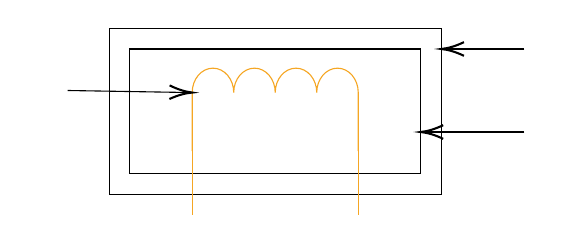
\begin{tikzpicture}[x=0.75pt,y=0.75pt,yscale=-1,xscale=1]
%uncomment if require: \path (0,300); %set diagram left start at 0, and has height of 300
%Shape: Rectangle [id:dp6431615116150586] 
\draw   (120,100) -- (260,100) -- (260,160) -- (120,160) -- cycle ;
%Shape: Rectangle [id:dp21722968746615745] 
\draw   (110,90) -- (270,90) -- (270,170) -- (110,170) -- cycle ;
%Shape: Inductor [id:dp2168804832907768] 
\draw  [color={rgb, 255:red, 245; green, 166; blue, 35 }  ,draw opacity=1 ] (150,149.24) -- (150,121) .. controls (150,114.51) and (154.48,109.24) .. (160,109.24) .. controls (165.52,109.24) and (170,114.51) .. (170,121) .. controls (170,114.51) and (174.48,109.24) .. (180,109.24) .. controls (185.52,109.24) and (190,114.51) .. (190,121) .. controls (190,114.51) and (194.48,109.24) .. (200,109.24) .. controls (205.52,109.24) and (210,114.51) .. (210,121) .. controls (210,114.51) and (214.48,109.24) .. (220,109.24) .. controls (225.52,109.24) and (230,114.51) .. (230,121) -- (230,149.24) ;
%Straight Lines [id:da9190346443391305] 
\draw [color={rgb, 255:red, 245; green, 166; blue, 35 }  ,draw opacity=1 ]   (150,149.24) -- (150,180) ;
%Straight Lines [id:da1556694134502471] 
\draw [color={rgb, 255:red, 245; green, 166; blue, 35 }  ,draw opacity=1 ]   (230,149.24) -- (230,180) ;
%Straight Lines [id:da6906822080495362] 
\draw    (90,120) -- (148,120.97) ;
\draw [shift={(150,121)}, rotate = 180.95] [color={rgb, 255:red, 0; green, 0; blue, 0 }  ][line width=0.75]    (10.93,-3.29) .. controls (6.95,-1.4) and (3.31,-0.3) .. (0,0) .. controls (3.31,0.3) and (6.95,1.4) .. (10.93,3.29)   ;
%Straight Lines [id:da8500651824334423] 
\draw    (310,100) -- (272,100) ;
\draw [shift={(270,100)}, rotate = 360] [color={rgb, 255:red, 0; green, 0; blue, 0 }  ][line width=0.75]    (10.93,-3.29) .. controls (6.95,-1.4) and (3.31,-0.3) .. (0,0) .. controls (3.31,0.3) and (6.95,1.4) .. (10.93,3.29)   ;
%Straight Lines [id:da6409885852889874] 
\draw    (310,140) -- (262,140) ;
\draw [shift={(260,140)}, rotate = 360] [color={rgb, 255:red, 0; green, 0; blue, 0 }  ][line width=0.75]    (10.93,-3.29) .. controls (6.95,-1.4) and (3.31,-0.3) .. (0,0) .. controls (3.31,0.3) and (6.95,1.4) .. (10.93,3.29)   ;

% Text Node
\draw (71,112) node [anchor=north west][inner sep=0.75pt]   [align=left] {\cstep\label{pas:1}};
% Text Node
\draw (318,132) node [anchor=north west][inner sep=0.75pt]   [align=left] {\cstep\label{pas:2}};
% Text Node
\draw (318,91) node [anchor=north west][inner sep=0.75pt]   [align=left] {\cstep\label{pas:3}};
\end{tikzpicture}
\end{figure}


\subsection{Dispositif Différentiel Résiduel\label{chap:DDR}}

\subsubsection{Caractéristiques générales}

\begin{definition}[Dispositif Différentiel Résiduel]
Un Dispositif Différentiel Résiduel (DDR) est un appareil de protection chargé d'assurer la protection des personnes contre les défauts d'isolement provoquant potentiellement des contacts indirects (\superref{def:contact_indirect}). Son rôle est de surveiller les fuites de courant d'une installation électrique vers la terre.
\end{definition}

Il convient de bien différencier deux type de DDR :
\begin{description}
\item[Interrupteur différentiel :] protection des personnes contre les contacts indirects dont le symbole est : \\
\begin{center}


\tikzset{every picture/.style={line width=0.75pt}} %set default line width to 0.75pt        

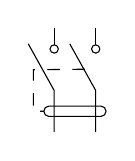
\begin{tikzpicture}[x=0.75pt,y=0.75pt,yscale=-1,xscale=1]
%uncomment if require: \path (0,300); %set diagram left start at 0, and has height of 300

%Straight Lines [id:da2903329919565012] 
\draw    (355,127.5) -- (367.5,150) -- (367.5,170) ;
%Shape: Circle [id:dp3187615529298826] 
\draw   (369.5,130) .. controls (369.5,128.9) and (368.6,128) .. (367.5,128) .. controls (366.4,128) and (365.5,128.9) .. (365.5,130) .. controls (365.5,131.1) and (366.4,132) .. (367.5,132) .. controls (368.6,132) and (369.5,131.1) .. (369.5,130) -- cycle ;
%Straight Lines [id:da6291068913098858] 
\draw    (367.5,128) -- (367.5,120) ;
%Rounded Rect [id:dp5228947876486602] 
\draw   (362.5,160) .. controls (362.5,158.62) and (363.62,157.5) .. (365,157.5) -- (390,157.5) .. controls (391.38,157.5) and (392.5,158.62) .. (392.5,160) -- (392.5,160) .. controls (392.5,161.38) and (391.38,162.5) .. (390,162.5) -- (365,162.5) .. controls (363.62,162.5) and (362.5,161.38) .. (362.5,160) -- cycle ;
%Straight Lines [id:da9535405775656056] 
\draw  [dash pattern={on 4.5pt off 4.5pt}]  (382.25,139.75) -- (357.5,140) -- (357.5,160) -- (362.5,160) ;
%Straight Lines [id:da293136389225495] 
\draw    (375,127.5) -- (387.5,150) -- (387.5,170) ;
%Shape: Circle [id:dp1387355280779735] 
\draw   (389.5,130) .. controls (389.5,128.9) and (388.6,128) .. (387.5,128) .. controls (386.4,128) and (385.5,128.9) .. (385.5,130) .. controls (385.5,131.1) and (386.4,132) .. (387.5,132) .. controls (388.6,132) and (389.5,131.1) .. (389.5,130) -- cycle ;
%Straight Lines [id:da810942314060853] 
\draw    (387.5,128) -- (387.5,120) ;

\end{tikzpicture}
\end{center}

\item[Disjoncteur différentiel :] protection des personnes contre les contacts indirects et protection des circuits contre les surintensités et les court-circuits dont le symbole est : \\
\begin{center}


\tikzset{every picture/.style={line width=0.75pt}} %set default line width to 0.75pt        

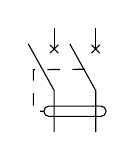
\begin{tikzpicture}[x=0.75pt,y=0.75pt,yscale=-1,xscale=1]
%uncomment if require: \path (0,300); %set diagram left start at 0, and has height of 300

%Straight Lines [id:da26208223112851936] 
\draw    (527.5,100) -- (540,122.5) -- (540,142.5) ;
%Straight Lines [id:da5822281275248988] 
\draw    (540,102.5) -- (540,92.5) ;
%Rounded Rect [id:dp41055324766610257] 
\draw   (535,132.5) .. controls (535,131.12) and (536.12,130) .. (537.5,130) -- (562.5,130) .. controls (563.88,130) and (565,131.12) .. (565,132.5) -- (565,132.5) .. controls (565,133.88) and (563.88,135) .. (562.5,135) -- (537.5,135) .. controls (536.12,135) and (535,133.88) .. (535,132.5) -- cycle ;
%Straight Lines [id:da30592283799275743] 
\draw  [dash pattern={on 4.5pt off 4.5pt}]  (554.75,112.25) -- (530,112.5) -- (530,132.5) -- (535,132.5) ;
%Straight Lines [id:da7841914077845515] 
\draw    (538,100.5) -- (542,104.5) ;
%Straight Lines [id:da01685582709758693] 
\draw    (542,100.5) -- (538,104.5) ;

%Straight Lines [id:da7197353055881572] 
\draw    (547.5,100) -- (560,122.5) -- (560,142.5) ;
%Straight Lines [id:da316262731013633] 
\draw    (560,102.5) -- (560,92.5) ;
%Straight Lines [id:da6806510311797901] 
\draw    (558,100.5) -- (562,104.5) ;
%Straight Lines [id:da5532087619463947] 
\draw    (562,100.5) -- (558,104.5) ;






\end{tikzpicture}

\end{center}
\end{description}

\begin{table}[h]
\caption{Valeur du seuil de $I_{\Delta n}$ fonction de $R_{A}$ et $U_{L}$}
\begin{tabularx}{\linewidth}{C i k S C i k S C i k S}
\toprule
\thead{$U_{L}$}	& \multicolumn{2}{c}{\thead{$R_{A}$ (\si{\ohm})}}	& 	{$I_{\Delta n}$ (\si{\ampere})}	& \thead{$U_{L}$}	& \multicolumn{2}{c}{\thead{$R_{A}$ (\si{\ohm})}}	& 	{$I_{\Delta n}$ (\si{\ampere})} & \thead{$U_{L}$}	& \multicolumn{2}{c}{\thead{$R_{A}$ (\si{\ohm})}}	& 	{$I_{\Delta n}$ (\si{\ampere})}	\\
\midrule
\SI{50}{\volt}	& \geq & 1660	&  0,030 		& \SI{25}{\volt}	& \geq & 500	& 	0,030	& \SI{12}{\volt}		& \geq & 400	&  0,030 \\
						& \geq & 166		&  0,300 		& 							& \geq & 83	&  0,300 	& 								& \geq & 40	&  0,300  \\
						& \geq & 100		&  0,500 		& 							& \geq & 50	&  0,500 	& 								& \geq & 24	&  0,500  \\
						& \geq & 16		&  3				& 							& \geq & 8		& 		 3 		& 								& \geq & 4		&  3  \\
\bottomrule
\end{tabularx}
\end{table}

\subsubsection{Marquage normalisé}

Comme tout appareil de protection, le DDR respecte des normes de qualité strictes (Conformité Européenne) et doivent présenter plusieurs marquages réglementaires, ainsi qu'un bouton \og TEST \fg{} pour informer l'installateur et l'utilisateur des caractéristiques du DDR. Cela informe de la conformité de l'appareil de protection.
\startcstep %remet les compteurs des légendes en pastille à zéro
\begin{center}
\begin{figure}[h]
\caption{Marquage d'un interrupteur différentiel}
\begin{subfigure}[t]{0.49\linewidth}
\subcaption{Vue de dessus}
\begin{annotate}
{\includegraphics[scale=1]{DDR_dessus}}{0.25}
%\helpgrid[gray] 
\node at (-11.8,4.3) {\cstep\label{pas:101}};
\node at (-11.8,2.2) {\cstep\label{pas:102}};
\node at (-11.8,-0.85) {\cstep\label{pas:103}};
\node at (-11.8,-3.85) {\cstep\label{pas:104}};
\node at (11.7,3.4) {\cstep\label{pas:105}};
\node at (11.7,1.1) {\cstep\label{pas:106}};
\node at (11.7,-2.1) {\cstep\label{pas:107}};
\end{annotate} 
\end{subfigure}
\begin{subfigure}[t]{0.49\linewidth}
\subcaption{Vue de dessus}
\begin{annotate}
{\includegraphics[scale=1]{DDR_avant}}{0.25}
%\helpgrid[gray] 
\node at (-11.8,6.7) {\cstep\label{pas:108}};
\node at (-11.8,3.8) {\cstep\label{pas:109}};
\node at (-11.9,-6.85) {\cstep\label{pas:110}};
\node at (11.7,3.85) {\cstep\label{pas:111}};
\node at (11.7,1) {\cstep\label{pas:112}};
\node at (11.7,-2.05) {\cstep\label{pas:113}};
\end{annotate} 
\end{subfigure}
\end{figure}
\end{center}
\begin{minipage}{\linewidth} %usage d'un environnement mini-page pour éviter les décalage au début de la première colonne quand l'élément n'est pas du texte simple
	\begin{multicols}{2} %répartition du texte dans l'environnement en deux colonnes
		\circref{pas:101}norme du produit\\ %légende automatique
		\circref{pas:102}tension assignée $230/400\si{\volt}\sim$\\
		\circref{pas:103}code de production\\
		\circref{pas:104}signe \og Courant assigné de court-circuit \SI{10000}{\ampere} \fg{} en combinaison avec un fusible en amont \\
		\circref{pas:105}pouvoir assigné de coupure \og \SI{1250}{\ampere} \fg{} \\
		\circref{pas:106}signe de sécurité ESTI (équivalent de la norme NF pour la Suisse) \\
		\circref{pas:107}signe \og Flocon de neige \fg{} (utilisation pour une température ambiante jusqu'à \SI{-25}{\degree}) \\
		\columnbreak\\ %passage à la deuxième colonne
		\circref{pas:108}couple de serrage \si{\newton\meter} \\
		\circref{pas:109}désignation du type\\
		\circref{pas:110}schéma des connexions\\
		\circref{pas:111}courant assigné $I_n$ de \SI{40}{\ampere} et calibre du DDR $I_{\Delta n}$\\
		\circref{pas:112}note concernant le test \og à effectuer tous les six mois \fg{}\\
		 \circref{pas:113}type de courant différentiel (type F)
	\end{multicols}
\end{minipage}


\subsubsection{Composante du courant de défaut}

Les DDR peuvent détecter plusieurs composantes du courant de défaut. C'est un paramètre qui peut varier selon le type d'appareil électrique protégé par le DDR.

%--------------------------------------
%ELECTROTECHNIQUE - SCHEMA DE LIAISON A LA TERRE
%--------------------------------------

%utiliser les environnement \begin{comment} \end{comment} pour mettre en commentaire le préambule une fois la programmation appelée dans le document maître (!ne pas oublier de mettre en commentaire \end{document}!)

\begin{comment}

\documentclass[a4paper, 11pt, twoside, fleqn]{memoir}

\usepackage{AOCDTF}

\input{marqueur_chapitre_couleur} %à personnaliser selon le nombre de chapitre dans le cours

%--------------------------------------
%corps du document
%--------------------------------------

\begin{document} %corps du document
	\openleft %début de chapitre à gauche

\end{comment}

\begin{xltabular}{\textwidth}{l c X c c }
\caption{Différents types de DDR selon les composantes du courant de défaut}\\
\toprule
\thead{Type}		& \thead{Symbole}		& \thead{Caractéristiques}	& \thead{Forme d'onde}		& \thead{Type de charge} \\
\midrule
\endfirsthead %en-tête de la première page du tableau  
\multicolumn{5}{l}{\small\textit{Page précédente}} \\
\midrule %filet de milieu de tableau
\thead{Type}		& \thead{Symbole}		& \thead{Caractéristiques}	& \thead{Forme d'onde}		& \thead{Type de charge} \\
\midrule
\endhead
\midrule %filet de milieu de tableau
\multicolumn{5}{r}{\small\textit{Page suivante}} \\
\endfoot %pied de page de toutes les pages du tableau
\bottomrule
\endlastfoot %pied de page de la dernièredu tableau
Type AC		& \adjustbox{valign=t}{\includegraphics[height=0.4cm]{type_ac.png}}		& 
\begin{tabitemize}
\item détection des courants alternatifs différentiels\,;
\item utilisation courante en domestique couvrant la plupart des besoin.
\end{tabitemize}
&

\adjustbox{valign=t}{

\tikzset{every picture/.style={line width=0.75pt}} %set default line width to 0.75pt        

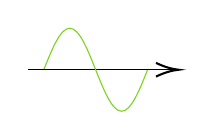
\begin{tikzpicture}[x=0.75pt,y=0.75pt,yscale=-1,xscale=1]
%uncomment if require: \path (0,57); %set diagram left start at 0, and has height of 57

%Straight Lines [id:da2943661507092279] 
\draw    (7.5,25) -- (78,25) ;
\draw [shift={(80,25)}, rotate = 180] [color={rgb, 255:red, 0; green, 0; blue, 0 }  ][line width=0.75]    (10.93,-3.29) .. controls (6.95,-1.4) and (3.31,-0.3) .. (0,0) .. controls (3.31,0.3) and (6.95,1.4) .. (10.93,3.29)   ;
%Shape: Wave [id:dp24323544196681968] 
\draw  [color={rgb, 255:red, 126; green, 211; blue, 33 }  ,draw opacity=1 ] (15,25) .. controls (19.08,14.75) and (22.98,5) .. (27.5,5) .. controls (32.02,5) and (35.92,14.75) .. (40,25) .. controls (44.08,35.25) and (47.98,45) .. (52.5,45) .. controls (57.02,45) and (60.92,35.25) .. (65,25) ;
%Straight Lines [id:da09599799976641754] 
\draw    (7.5,25) -- (30,25) ;
%Straight Lines [id:da7289357219255289] 
\draw    (43.75,25) -- (66.25,25) ;


\end{tikzpicture}}
 &
 
\adjustbox{valign=t}{


\tikzset{every picture/.style={line width=0.75pt}} %set default line width to 0.75pt        

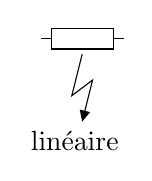
\begin{tikzpicture}[x=0.75pt,y=0.75pt,yscale=-1,xscale=1]
%uncomment if require: \path (0,98); %set diagram left start at 0, and has height of 98

%Straight Lines [id:da7324284340679806] 
\draw    (122.5,17.5) -- (127.5,17.5) ;
%Shape: Rectangle [id:dp18713096911447358] 
\draw   (92.5,12.5) -- (122.5,12.5) -- (122.5,22.5) -- (92.5,22.5) -- cycle ;
%Straight Lines [id:da2214074924221885] 
\draw    (87.5,17.5) -- (92.5,17.5) ;

%Straight Lines [id:da09102665939260723] 
\draw    (107.5,25) -- (102.5,45) -- (112.5,37.5) -- (108.23,54.59) ;
\draw [shift={(107.5,57.5)}, rotate = 284.04] [fill={rgb, 255:red, 0; green, 0; blue, 0 }  ][line width=0.08]  [draw opacity=0] (5.36,-2.57) -- (0,0) -- (5.36,2.57) -- cycle    ;

% Text Node
\draw (81.5,61) node [anchor=north west][inner sep=0.75pt]   [align=left] {linéaire};


\end{tikzpicture}}

  \\
    \addlinespace
  \addlinespace

  
  
  Type A		& \adjustbox{valign=t}{\includegraphics[height=0.4cm]{type_a.png}}		& 
\begin{tabitemize}
\item détection des courants différentiels alternatifs et des courants différentiels continus pulsés\,;
\item utilisation spécifique pour les charges électriques monophasées de type 1.
\end{tabitemize}
&

\adjustbox{valign=t}{




\tikzset{every picture/.style={line width=0.75pt}} %set default line width to 0.75pt        

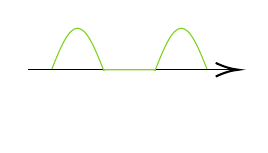
\begin{tikzpicture}[x=0.75pt,y=0.75pt,yscale=-1,xscale=1]
%uncomment if require: \path (0,108); %set diagram left start at 0, and has height of 108

%Shape: Wave [id:dp27700594343461393] 
\draw  [color={rgb, 255:red, 126; green, 211; blue, 33 }  ,draw opacity=1 ] (35,45) .. controls (39.08,34.75) and (42.98,25) .. (47.5,25) .. controls (52.02,25) and (55.92,34.75) .. (60,45) .. controls (64.08,55.25) and (67.98,65) .. (72.5,65) .. controls (77.02,65) and (80.92,55.25) .. (85,45) .. controls (89.08,34.75) and (92.98,25) .. (97.5,25) .. controls (102.02,25) and (105.92,34.75) .. (110,45) ;
%Straight Lines [id:da5910455205676639] 
\draw    (23.75,45) -- (123,45) ;
\draw [shift={(125,45)}, rotate = 180] [color={rgb, 255:red, 0; green, 0; blue, 0 }  ][line width=0.75]    (10.93,-3.29) .. controls (6.95,-1.4) and (3.31,-0.3) .. (0,0) .. controls (3.31,0.3) and (6.95,1.4) .. (10.93,3.29)   ;
%Straight Lines [id:da5095890041059973] 
\draw [color={rgb, 255:red, 126; green, 211; blue, 33 }  ,draw opacity=1 ]   (60,45) -- (85,45) ;
%Shape: Trapezoid [id:dp9576415302257589] 
\draw  [color={rgb, 255:red, 126; green, 211; blue, 33 }  ,draw opacity=1 ] (85,45) -- (84.7,46) -- (60.3,46) -- (60,45) -- cycle ;
%Shape: Rectangle [id:dp7690910497329457] 
\draw  [draw opacity=0][fill={rgb, 255:red, 255; green, 255; blue, 255 }  ,fill opacity=1 ][line width=5.25]  (35,45.5) -- (105,45.5) -- (105,68) -- (35,68) -- cycle ;




\end{tikzpicture}

}
 &
 
 
\adjustbox{valign=t}{



\tikzset{every picture/.style={line width=0.75pt}} %set default line width to 0.75pt        

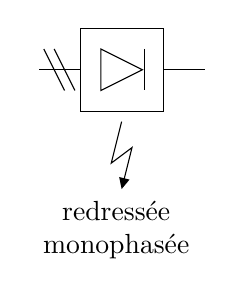
\begin{tikzpicture}[x=0.75pt,y=0.75pt,yscale=-1,xscale=1]
%uncomment if require: \path (0,152); %set diagram left start at 0, and has height of 152

%Straight Lines [id:da2993135281874989] 
\draw    (40,35) -- (30,15) ;
%Straight Lines [id:da1407255659834652] 
\draw    (35,35) -- (25,15) ;
%Straight Lines [id:da0646281171352201] 
\draw    (42.5,25) -- (22.5,25) ;
%Shape: Square [id:dp8095195384599084] 
\draw   (42.5,5) -- (82.5,5) -- (82.5,45) -- (42.5,45) -- cycle ;
%Shape: Boxed Line [id:dp9015036881777688] 
\draw    (73.5,15) -- (73.5,35) ;
%Shape: Triangle [id:dp25930553779074683] 
\draw   (72.5,25) -- (52.5,35) -- (52.5,15) -- cycle ;
%Straight Lines [id:da624315601423471] 
\draw    (62.5,50) -- (57.5,70) -- (67.5,62.5) -- (63.23,79.59) ;
\draw [shift={(62.5,82.5)}, rotate = 284.04] [fill={rgb, 255:red, 0; green, 0; blue, 0 }  ][line width=0.08]  [draw opacity=0] (5.36,-2.57) -- (0,0) -- (5.36,2.57) -- cycle    ;
%Straight Lines [id:da583175718122269] 
\draw    (102.5,25) -- (82.5,25) ;

% Text Node
\draw (17.5,87) node [anchor=north west][inner sep=0.75pt]   [align=left] {\begin{minipage}[lt]{61.699375pt}\setlength\topsep{0pt}
\begin{center}
redressée\\monophasée
\end{center}

\end{minipage}};


\end{tikzpicture}
}

  \\
    \addlinespace
  \addlinespace

  
    Type F		& \adjustbox{valign=t}{\includegraphics[height=0.4cm]{type_f.png}}		& 
\begin{tabitemize}
\item détection des courants différentiels alternatifs, les courants différentiels continus pulsés et les courants différentiels de fréquences mixtes jusqu'à \SI{1}{\kilo\hertz}\,;
\item utilisation spécifique pour circuits comportant des variateurs de vitesse monophasés.
\end{tabitemize}
&

\adjustbox{valign=t}{
\tikzset{every picture/.style={line width=0.75pt}} %set default line width to 0.75pt        

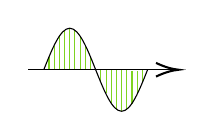
\begin{tikzpicture}[x=0.75pt,y=0.75pt,yscale=-1,xscale=1]
%uncomment if require: \path (0,108); %set diagram left start at 0, and has height of 108

%Straight Lines [id:da8344481258673822] 
\draw [color={rgb, 255:red, 126; green, 211; blue, 33 }  ,draw opacity=1 ]   (47.5,25) -- (47.5,45) ;
%Straight Lines [id:da45734535299498047] 
\draw [color={rgb, 255:red, 126; green, 211; blue, 33 }  ,draw opacity=1 ]   (45,26) -- (45,45) ;
%Straight Lines [id:da4148698837495829] 
\draw [color={rgb, 255:red, 126; green, 211; blue, 33 }  ,draw opacity=1 ]   (42.5,28.5) -- (42.5,44.5) ;
%Straight Lines [id:da9637733631041641] 
\draw [color={rgb, 255:red, 126; green, 211; blue, 33 }  ,draw opacity=1 ]   (37.5,39) -- (37.5,45) ;
%Straight Lines [id:da15505371109761856] 
\draw [color={rgb, 255:red, 126; green, 211; blue, 33 }  ,draw opacity=1 ]   (40,33.5) -- (40,44.5) ;
%Straight Lines [id:da8124028319543418] 
\draw [color={rgb, 255:red, 126; green, 211; blue, 33 }  ,draw opacity=1 ]   (52.5,29) -- (52.5,45) ;
%Straight Lines [id:da9805020896518191] 
\draw [color={rgb, 255:red, 126; green, 211; blue, 33 }  ,draw opacity=1 ]   (50,26) -- (50,45) ;
%Straight Lines [id:da4116431840997269] 
\draw [color={rgb, 255:red, 126; green, 211; blue, 33 }  ,draw opacity=1 ]   (55,34) -- (55,45) ;
%Straight Lines [id:da8823890585871352] 
\draw [color={rgb, 255:red, 126; green, 211; blue, 33 }  ,draw opacity=1 ]   (57.5,39) -- (57.5,45) ;
%Straight Lines [id:da9104778326348498] 
\draw [color={rgb, 255:red, 126; green, 211; blue, 33 }  ,draw opacity=1 ]   (72.5,65) -- (72.5,45) ;
%Straight Lines [id:da36879417192210706] 
\draw [color={rgb, 255:red, 126; green, 211; blue, 33 }  ,draw opacity=1 ]   (75,64) -- (75,45) ;
%Straight Lines [id:da056894793071553984] 
\draw [color={rgb, 255:red, 126; green, 211; blue, 33 }  ,draw opacity=1 ]   (77.5,61.5) -- (77.5,45.5) ;
%Straight Lines [id:da926320044180968] 
\draw [color={rgb, 255:red, 126; green, 211; blue, 33 }  ,draw opacity=1 ]   (82.5,51) -- (82.5,45) ;
%Straight Lines [id:da4802255081072313] 
\draw [color={rgb, 255:red, 126; green, 211; blue, 33 }  ,draw opacity=1 ]   (80,56.5) -- (80,45.5) ;
%Straight Lines [id:da8191961490083182] 
\draw [color={rgb, 255:red, 126; green, 211; blue, 33 }  ,draw opacity=1 ]   (67.5,61) -- (67.5,45) ;
%Straight Lines [id:da2923358818287347] 
\draw [color={rgb, 255:red, 126; green, 211; blue, 33 }  ,draw opacity=1 ]   (70,64) -- (70,45) ;
%Straight Lines [id:da3136693713803336] 
\draw [color={rgb, 255:red, 126; green, 211; blue, 33 }  ,draw opacity=1 ]   (65,56) -- (65,45) ;
%Straight Lines [id:da549046744886196] 
\draw [color={rgb, 255:red, 126; green, 211; blue, 33 }  ,draw opacity=1 ]   (62.5,51) -- (62.5,45) ;

%Shape: Wave [id:dp9341521104203707] 
\draw  [color={rgb, 255:red, 0; green, 0; blue, 0 }  ,draw opacity=1 ] (35,45) .. controls (39.08,34.75) and (42.98,25) .. (47.5,25) .. controls (52.02,25) and (55.92,34.75) .. (60,45) .. controls (64.08,55.25) and (67.98,65) .. (72.5,65) .. controls (77.02,65) and (80.92,55.25) .. (85,45) ;
%Straight Lines [id:da8093364598636541] 
\draw    (27.5,45) -- (98,45) ;
\draw [shift={(100,45)}, rotate = 180] [color={rgb, 255:red, 0; green, 0; blue, 0 }  ][line width=0.75]    (10.93,-3.29) .. controls (6.95,-1.4) and (3.31,-0.3) .. (0,0) .. controls (3.31,0.3) and (6.95,1.4) .. (10.93,3.29)   ;




\end{tikzpicture}

}
 &
 
 
\adjustbox{valign=t}{


\tikzset{every picture/.style={line width=0.75pt}} %set default line width to 0.75pt        

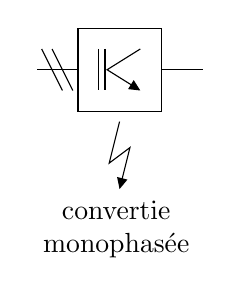
\begin{tikzpicture}[x=0.75pt,y=0.75pt,yscale=-1,xscale=1]
%uncomment if require: \path (0,152); %set diagram left start at 0, and has height of 152

%Straight Lines [id:da2004774518549749] 
\draw    (40,35) -- (30,15) ;
%Straight Lines [id:da28878490688185077] 
\draw    (35,35) -- (25,15) ;
%Straight Lines [id:da28622017833538005] 
\draw    (42.5,25) -- (22.5,25) ;
%Straight Lines [id:da27361779183994883] 
\draw    (62.5,50) -- (57.5,70) -- (67.5,62.5) -- (63.23,79.59) ;
\draw [shift={(62.5,82.5)}, rotate = 284.04] [fill={rgb, 255:red, 0; green, 0; blue, 0 }  ][line width=0.08]  [draw opacity=0] (5.36,-2.57) -- (0,0) -- (5.36,2.57) -- cycle    ;
%Straight Lines [id:da3667194527320474] 
\draw    (102.5,25) -- (82.5,25) ;
%Shape: Square [id:dp27983484657325586] 
\draw   (42.5,5) -- (82.5,5) -- (82.5,45) -- (42.5,45) -- cycle ;
%Shape: Boxed Line [id:dp856307990834614] 
\draw    (52.5,15) -- (52.5,35) ;
%Straight Lines [id:da34232786335443943] 
\draw    (72.5,15) -- (56.5,25) -- (69.96,33.41) ;
\draw [shift={(72.5,35)}, rotate = 212.01] [fill={rgb, 255:red, 0; green, 0; blue, 0 }  ][line width=0.08]  [draw opacity=0] (5.36,-2.57) -- (0,0) -- (5.36,2.57) -- cycle    ;
%Shape: Boxed Line [id:dp1790472061066909] 
\draw    (55.5,15) -- (55.5,35) ;


% Text Node
\draw (18.5,87) node [anchor=north west][inner sep=0.75pt]   [align=left] {\begin{minipage}[lt]{61.699375pt}\setlength\topsep{0pt}
\begin{center}
convertie\\monophasée
\end{center}

\end{minipage}};


\end{tikzpicture}

}

  \\
    \addlinespace
        \addlinespace


      Type B		& \adjustbox{valign=t}{\includegraphics[height=0.4cm]{type_b.png}}		& 
\begin{tabitemize}
\item détection des courants différentiels alternatifs, les courants différentiels continus pulsés, des courants différentiels de fréquences mixtes jusqu'à \SI{1}{\kilo\hertz} et des courants différentiels continus lisses\,;
\item utilisation spécifique pour circuits comportant des variateurs de vitesse triphasés, un système photovoltaïque, une borne de recharge de véhicule électrique ou encore des équipements médicaux.
\end{tabitemize}
&

\adjustbox{valign=t}{


\tikzset{every picture/.style={line width=0.75pt}} %set default line width to 0.75pt        

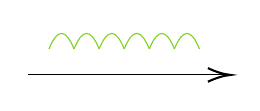
\begin{tikzpicture}[x=0.75pt,y=0.75pt,yscale=-1,xscale=1]
%uncomment if require: \path (0,108); %set diagram left start at 0, and has height of 108

%Straight Lines [id:da7026343722095999] 
\draw    (47.5,87.5) -- (143,87.5) ;
\draw [shift={(145,87.5)}, rotate = 180] [color={rgb, 255:red, 0; green, 0; blue, 0 }  ][line width=0.75]    (10.93,-3.29) .. controls (6.95,-1.4) and (3.31,-0.3) .. (0,0) .. controls (3.31,0.3) and (6.95,1.4) .. (10.93,3.29)   ;
%Shape: Parabola [id:dp4469234992699831] 
\draw  [color={rgb, 255:red, 126; green, 211; blue, 33 }  ,draw opacity=1 ] (69.58,75) .. controls (65.55,65) and (61.52,65) .. (57.5,75) ;
%Shape: Parabola [id:dp10691023078597706] 
\draw  [color={rgb, 255:red, 126; green, 211; blue, 33 }  ,draw opacity=1 ] (81.67,75) .. controls (77.64,65) and (73.61,65) .. (69.58,75) ;
%Shape: Parabola [id:dp9540942461898068] 
\draw  [color={rgb, 255:red, 126; green, 211; blue, 33 }  ,draw opacity=1 ] (93.75,75) .. controls (89.73,65) and (85.7,65) .. (81.67,75) ;
%Shape: Parabola [id:dp6220203064360257] 
\draw  [color={rgb, 255:red, 126; green, 211; blue, 33 }  ,draw opacity=1 ] (105.83,75) .. controls (101.8,65) and (97.77,65) .. (93.75,75) ;
%Shape: Parabola [id:dp4992966008122459] 
\draw  [color={rgb, 255:red, 126; green, 211; blue, 33 }  ,draw opacity=1 ] (117.92,75) .. controls (113.89,65) and (109.86,65) .. (105.83,75) ;
%Shape: Parabola [id:dp01154198803526707] 
\draw  [color={rgb, 255:red, 126; green, 211; blue, 33 }  ,draw opacity=1 ] (130,75) .. controls (125.98,65) and (121.95,65) .. (117.92,75) ;




\end{tikzpicture}

}
 &
 
 
\adjustbox{valign=t}{


\tikzset{every picture/.style={line width=0.75pt}} %set default line width to 0.75pt        

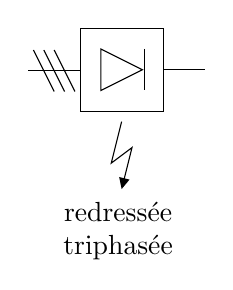
\begin{tikzpicture}[x=0.75pt,y=0.75pt,yscale=-1,xscale=1]
%uncomment if require: \path (0,141); %set diagram left start at 0, and has height of 141

%Straight Lines [id:da4147930693711671] 
\draw    (60,42.5) -- (50,22.5) ;
%Straight Lines [id:da7913487771488718] 
\draw    (55,42.5) -- (45,22.5) ;
%Straight Lines [id:da12782809797617567] 
\draw    (62.5,32.5) -- (37.5,32.5) ;
%Shape: Square [id:dp3051019253176962] 
\draw   (62.5,12) -- (102.5,12) -- (102.5,52) -- (62.5,52) -- cycle ;
%Shape: Boxed Line [id:dp3719227311734635] 
\draw    (93.5,22) -- (93.5,42) ;
%Shape: Triangle [id:dp5734231710257448] 
\draw   (92.5,32) -- (72.5,42) -- (72.5,22) -- cycle ;
%Straight Lines [id:da20189459286959577] 
\draw    (82.5,57) -- (77.5,77) -- (87.5,69.5) -- (83.23,86.59) ;
\draw [shift={(82.5,89.5)}, rotate = 284.04] [fill={rgb, 255:red, 0; green, 0; blue, 0 }  ][line width=0.08]  [draw opacity=0] (5.36,-2.57) -- (0,0) -- (5.36,2.57) -- cycle    ;
%Straight Lines [id:da8309944422064088] 
\draw    (122.5,32) -- (102.5,32) ;
%Straight Lines [id:da522665354082454] 
\draw    (50,42.5) -- (40,22.5) ;

% Text Node
\draw (47.5,94.5) node [anchor=north west][inner sep=0.75pt]   [align=left] {\begin{minipage}[lt]{48.078125pt}\setlength\topsep{0pt}
\begin{center}
redressée\\triphasée
\end{center}

\end{minipage}};


\end{tikzpicture}


}

  \\
  \addlinespace
  
\end{xltabular}


%\end{document}



\subsubsection{Principe de fonctionnement}

Les éléments essentiels d'un DDR sont les suivants : \\
\begin{minipage}{\linewidth} %usage d'un environnement mini-page pour éviter les décalage au début de la première colonne quand l'élément n'est pas du texte simple
	\begin{multicols}{2} %répartition du texte dans l'environnement en deux colonnes
	\startcstep %remet les compteurs des légendes en pastille à zéro
		\circref{pas:20} bouton test d'essai du DDR\\ %légende automatique
		\circref{pas:21} transformateur d'intensité (tore de détection)\\
		\circref{pas:22} relais de déclenchement  \\
		\circref{pas:23} mécanisme à déclenchement libre sans retour automatique \\
		\columnbreak\\ %passage à la deuxième colonne
		$I_1$ : courant \og d'arrivée \fg{} du récepteur \\
		$I_2$ : courant \og de sortie \fg{} du récepteur \\
		$I_d$ : courant de défaut\\
		$I_c$ : courant de contact\\
		$R_b$ : résistance de terre du neutre\\
		$R_a$ : résistance de la prise de terre de l'installation électrique 
	\end{multicols}
\end{minipage}
~\\
Pour le fonctionnement d'un DDR, les conditions suivantes doivent être remplie :
\begin{itemize}
\item le point neutre du transformateur HT/BT doit être mis à la terre\,;
\item aucune liaison entre le conducteur de neutre et le conducteur de protection ne doit être réalisée en aval du DDR\,;
\item le conducteur de protection ne doit pas transiter dans le transformateur d'intensité\,;
\item le réseau doit être alternatif.
\end{itemize}

%--------------------------------------
%ELECTROTECHNIQUE - SCHEMA DE LIAISON A LA TERRE
%--------------------------------------

%utiliser les environnement \begin{comment} \end{comment} pour mettre en commentaire le préambule une fois la programmation appelée dans le document maître (!ne pas oublier de mettre en commentaire \end{document}!)

\begin{comment}

\documentclass[a4paper, 11pt, twoside, fleqn]{memoir}

\usepackage{AOCDTF}

\marqueurchapitre

%lien d'édition des figures Tikz sur le site mathcha.io (rajouter le lien d'une modification effectuée sur la figure tikz avec le nom du modificateur car il n'y a qu'un lien par compte)

%lien mathcha Bruno Douchy : https://www.mathcha.io/editor/Bk7MWCBDtnqu2XZxxvhXxLngrckymkMKHgN9PBn

%--------------------------------------
%corps du document
%--------------------------------------

\begin{document} %corps du document
	\openleft %début de chapitre à gauche

\end{comment}

\begin{figure}[h]
\caption{Principe de fonctionnement d'un DDR}
% Pattern Info
 
\tikzset{
pattern size/.store in=\mcSize, 
pattern size = 5pt,
pattern thickness/.store in=\mcThickness, 
pattern thickness = 0.3pt,
pattern radius/.store in=\mcRadius, 
pattern radius = 1pt}
\makeatletter
\pgfutil@ifundefined{pgf@pattern@name@_ord9zgesw}{
\pgfdeclarepatternformonly[\mcThickness,\mcSize]{_ord9zgesw}
{\pgfqpoint{0pt}{0pt}}
{\pgfpoint{\mcSize+\mcThickness}{\mcSize+\mcThickness}}
{\pgfpoint{\mcSize}{\mcSize}}
{
\pgfsetcolor{\tikz@pattern@color}
\pgfsetlinewidth{\mcThickness}
\pgfpathmoveto{\pgfqpoint{0pt}{0pt}}
\pgfpathlineto{\pgfpoint{\mcSize+\mcThickness}{\mcSize+\mcThickness}}
\pgfusepath{stroke}
}}
\makeatother
\tikzset{every picture/.style={line width=0.75pt}} %set default line width to 0.75pt        

\begin{tikzpicture}[x=0.75pt,y=0.75pt,yscale=-1,xscale=1]
%uncomment if require: \path (0,424); %set diagram left start at 0, and has height of 424

%Straight Lines [id:da8966163314767044] 
\draw [color={rgb, 255:red, 248; green, 231; blue, 28 }  ,draw opacity=1 ]   (87.5,347.5) -- (87.5,372.5) ;
%Straight Lines [id:da7222083613228029] 
\draw [color={rgb, 255:red, 248; green, 231; blue, 28 }  ,draw opacity=1 ]   (222.5,260) -- (207.5,260) -- (207.5,307.5) ;
%Straight Lines [id:da23218758522860672] 
\draw    (170.5,77) -- (192.5,75) -- (202.5,75) ;
%Straight Lines [id:da7512535542730762] 
\draw    (172.5,75) -- (162.5,75) ;
%Straight Lines [id:da4548446207037964] 
\draw    (170.5,77) -- (174.5,73) ;
%Straight Lines [id:da048652925498270605] 
\draw    (170.5,73) -- (174.5,77) ;

%Straight Lines [id:da7240820211401438] 
\draw    (170.5,57) -- (192.5,55) -- (202.5,55) ;
%Straight Lines [id:da3532902355954177] 
\draw    (172.5,55) -- (162.5,55) ;
%Straight Lines [id:da3444450540631401] 
\draw    (170.5,57) -- (174.5,53) ;
%Straight Lines [id:da5449997149390995] 
\draw    (170.5,53) -- (174.5,57) ;

%Straight Lines [id:da8409656810439277] 
\draw  [dash pattern={on 4.5pt off 4.5pt}]  (181.5,76) -- (181.5,16) ;
%Straight Lines [id:da3313477668587995] 
\draw    (170.5,37) -- (192.5,35) -- (202.5,35) ;
%Straight Lines [id:da046033439865870274] 
\draw    (172.5,35) -- (162.5,35) ;
%Straight Lines [id:da32442953656655926] 
\draw    (170.5,37) -- (174.5,33) ;
%Straight Lines [id:da6384518069767443] 
\draw    (170.5,33) -- (174.5,37) ;

%Straight Lines [id:da9876100878122998] 
\draw    (170.5,17) -- (192.5,15) -- (202.5,15) ;
%Straight Lines [id:da9878077133650999] 
\draw    (172.5,15) -- (162.5,15) ;
%Straight Lines [id:da8400535804483228] 
\draw    (170.5,17) -- (174.5,13) ;
%Straight Lines [id:da07115708140229215] 
\draw    (170.5,13) -- (174.5,17) ;


%Straight Lines [id:da7042823655297029] 
\draw    (120,35) -- (162.5,35) ;
%Straight Lines [id:da4916339989794427] 
\draw [color={rgb, 255:red, 139; green, 87; blue, 42 }  ,draw opacity=1 ]   (112.5,15) -- (162.5,15) ;
%Straight Lines [id:da444327748342345] 
\draw [color={rgb, 255:red, 155; green, 155; blue, 155 }  ,draw opacity=1 ]   (112.5,55) -- (162.5,55) ;
%Straight Lines [id:da8096274481374413] 
\draw [color={rgb, 255:red, 74; green, 144; blue, 226 }  ,draw opacity=1 ]   (87.5,75) -- (162.5,75) ;
%Straight Lines [id:da255508302316241] 
\draw [color={rgb, 255:red, 248; green, 231; blue, 28 }  ,draw opacity=1 ]   (95.5,35) -- (87.5,65) -- (87.5,307.5) ;
%Straight Lines [id:da6402263719803258] 
\draw [color={rgb, 255:red, 126; green, 211; blue, 33 }  ,draw opacity=1 ] [dash pattern={on 4.5pt off 4.5pt }]  (95.5,35) -- (87.5,65) -- (87.5,161.33) -- (87.5,307.5) ;
%Shape: Circle [id:dp3717655452004347] 
\draw  [fill={rgb, 255:red, 0; green, 0; blue, 0 }  ,fill opacity=1 ] (85,75) .. controls (85,73.62) and (86.12,72.5) .. (87.5,72.5) .. controls (88.88,72.5) and (90,73.62) .. (90,75) .. controls (90,76.38) and (88.88,77.5) .. (87.5,77.5) .. controls (86.12,77.5) and (85,76.38) .. (85,75) -- cycle ;
%Straight Lines [id:da2541613595150951] 
\draw    (202.5,35) -- (460,35) ;
%Straight Lines [id:da3042036157593445] 
\draw [color={rgb, 255:red, 139; green, 87; blue, 42 }  ,draw opacity=1 ]   (202.5,15) -- (460,15) ;
%Straight Lines [id:da7230237325510261] 
\draw [color={rgb, 255:red, 155; green, 155; blue, 155 }  ,draw opacity=1 ]   (202.5,55) -- (460,55) ;
%Straight Lines [id:da12677288022811684] 
\draw [color={rgb, 255:red, 74; green, 144; blue, 226 }  ,draw opacity=1 ]   (202.5,75) -- (460,75) ;
%Shape: Path Data [id:dp12072280734027463] 
\draw   (112.5,55) .. controls (112.5,56.38) and (111.38,57.5) .. (110,57.5) .. controls (109.29,57.5) and (108.65,57.2) .. (108.19,56.72) .. controls (102.81,61.85) and (95.52,65) .. (87.5,65) .. controls (70.93,65) and (57.5,51.57) .. (57.5,35) .. controls (57.5,18.43) and (70.93,5) .. (87.5,5) .. controls (95.52,5) and (102.81,8.15) .. (108.19,13.28) .. controls (108.65,12.8) and (109.29,12.5) .. (110,12.5) .. controls (111.38,12.5) and (112.5,13.62) .. (112.5,15) .. controls (112.5,15.82) and (112.11,16.54) .. (111.5,17) .. controls (114.8,21.39) and (116.92,26.71) .. (117.4,32.5) .. controls (117.43,32.5) and (117.47,32.5) .. (117.5,32.5) .. controls (118.88,32.5) and (120,33.62) .. (120,35) .. controls (120,36.38) and (118.88,37.5) .. (117.5,37.5) .. controls (117.47,37.5) and (117.43,37.5) .. (117.4,37.5) .. controls (116.92,43.29) and (114.8,48.61) .. (111.5,53) .. controls (112.11,53.46) and (112.5,54.18) .. (112.5,55) -- cycle ;
%Shape: Circle [id:dp9132632008322901] 
\draw   (17.5,35) .. controls (17.5,18.43) and (30.93,5) .. (47.5,5) .. controls (64.07,5) and (77.5,18.43) .. (77.5,35) .. controls (77.5,51.57) and (64.07,65) .. (47.5,65) .. controls (30.93,65) and (17.5,51.57) .. (17.5,35) -- cycle ;
%Shape: Triangle [id:dp10434360164177936] 
\draw   (40,25) -- (30,42.5) -- (50,42.5) -- cycle ;
%Shape: Star [id:dp8894948986285862] 
\draw   (106.75,35) -- (95.5,35) -- (89.88,44.81) -- (95.5,35) -- (89.88,25.19) -- (95.5,35) -- cycle ;
%Shape: Circle [id:dp32709816081021414] 
\draw   (107.5,15) .. controls (107.5,13.62) and (108.62,12.5) .. (110,12.5) .. controls (111.38,12.5) and (112.5,13.62) .. (112.5,15) .. controls (112.5,16.38) and (111.38,17.5) .. (110,17.5) .. controls (108.62,17.5) and (107.5,16.38) .. (107.5,15) -- cycle ;
%Shape: Circle [id:dp5474750610722358] 
\draw   (114.9,35) .. controls (114.9,33.62) and (116.02,32.5) .. (117.4,32.5) .. controls (118.78,32.5) and (119.9,33.62) .. (119.9,35) .. controls (119.9,36.38) and (118.78,37.5) .. (117.4,37.5) .. controls (116.02,37.5) and (114.9,36.38) .. (114.9,35) -- cycle ;
%Shape: Circle [id:dp9648369805697471] 
\draw   (107.5,55) .. controls (107.5,53.62) and (108.62,52.5) .. (110,52.5) .. controls (111.38,52.5) and (112.5,53.62) .. (112.5,55) .. controls (112.5,56.38) and (111.38,57.5) .. (110,57.5) .. controls (108.62,57.5) and (107.5,56.38) .. (107.5,55) -- cycle ;

%Shape: Circle [id:dp8028626789087734] 
\draw  [fill={rgb, 255:red, 0; green, 0; blue, 0 }  ,fill opacity=1 ] (250,15) .. controls (250,13.62) and (251.12,12.5) .. (252.5,12.5) .. controls (253.88,12.5) and (255,13.62) .. (255,15) .. controls (255,16.38) and (253.88,17.5) .. (252.5,17.5) .. controls (251.12,17.5) and (250,16.38) .. (250,15) -- cycle ;
%Straight Lines [id:da6710342602087992] 
\draw [color={rgb, 255:red, 139; green, 87; blue, 42 }  ,draw opacity=1 ]   (252.5,102.5) -- (252.5,17.5) ;
%Straight Lines [id:da1721071364007184] 
\draw    (249.5,110) -- (252.5,132.5) -- (252.5,142.5) ;
%Shape: Circle [id:dp9426602450789092] 
\draw   (254.5,112.5) .. controls (254.5,111.4) and (253.6,110.5) .. (252.5,110.5) .. controls (251.4,110.5) and (250.5,111.4) .. (250.5,112.5) .. controls (250.5,113.6) and (251.4,114.5) .. (252.5,114.5) .. controls (253.6,114.5) and (254.5,113.6) .. (254.5,112.5) -- cycle ;
%Straight Lines [id:da760907905232019] 
\draw    (252.5,110.5) -- (252.5,102.5) ;
%Straight Lines [id:da24434047675058257] 
\draw [color={rgb, 255:red, 74; green, 144; blue, 226 }  ,draw opacity=1 ]   (292.5,102.5) -- (292.5,77.5) ;
%Shape: Circle [id:dp6617550715428236] 
\draw   (294.5,112.5) .. controls (294.5,111.4) and (293.6,110.5) .. (292.5,110.5) .. controls (291.4,110.5) and (290.5,111.4) .. (290.5,112.5) .. controls (290.5,113.6) and (291.4,114.5) .. (292.5,114.5) .. controls (293.6,114.5) and (294.5,113.6) .. (294.5,112.5) -- cycle ;
%Straight Lines [id:da17662194069433912] 
\draw    (292.5,110.5) -- (292.5,102.5) ;
%Shape: Can [id:dp4099150432020693] 
\draw   (313,173.75) -- (313,186.25) .. controls (313,189.7) and (296.21,192.5) .. (275.5,192.5) .. controls (254.79,192.5) and (238,189.7) .. (238,186.25) -- (238,173.75) .. controls (238,170.3) and (254.79,167.5) .. (275.5,167.5) .. controls (296.21,167.5) and (313,170.3) .. (313,173.75) .. controls (313,177.2) and (296.21,180) .. (275.5,180) .. controls (254.79,180) and (238,177.2) .. (238,173.75) ;
%Shape: Ellipse [id:dp9432226775402133] 
\draw   (247.5,173) .. controls (247.5,170.79) and (259.81,169) .. (275,169) .. controls (290.19,169) and (302.5,170.79) .. (302.5,173) .. controls (302.5,175.21) and (290.19,177) .. (275,177) .. controls (259.81,177) and (247.5,175.21) .. (247.5,173) -- cycle ;
%Straight Lines [id:da3842385283784233] 
\draw    (289.5,110) -- (292.5,132.5) -- (292.5,142.5) ;
%Straight Lines [id:da020374420940482918] 
\draw [color={rgb, 255:red, 74; green, 144; blue, 226 }  ,draw opacity=1 ]   (292.5,175) -- (292.5,142.5) ;
%Straight Lines [id:da4986320001259672] 
\draw [color={rgb, 255:red, 139; green, 87; blue, 42 }  ,draw opacity=1 ]   (252.5,175) -- (252.5,142.5) ;
%Curve Lines [id:da4474262405289132] 
\draw [color={rgb, 255:red, 139; green, 87; blue, 42 }  ,draw opacity=1 ]   (249.5,175) .. controls (235.5,163) and (231.5,201) .. (242.5,190) ;
%Curve Lines [id:da3440642000821973] 
\draw [color={rgb, 255:red, 139; green, 87; blue, 42 }  ,draw opacity=1 ]   (252.5,176) .. controls (239.5,163) and (232.5,203) .. (245.5,190) ;
%Curve Lines [id:da23911359335186] 
\draw [color={rgb, 255:red, 139; green, 87; blue, 42 }  ,draw opacity=1 ]   (255.5,176.5) .. controls (248.83,169.83) and (244.01,176.71) .. (242.51,183.45) .. controls (241.08,189.84) and (242.66,196.1) .. (248.5,190.5) ;
%Curve Lines [id:da6529791777103667] 
\draw [color={rgb, 255:red, 139; green, 87; blue, 42 }  ,draw opacity=1 ]   (248,172.5) .. controls (235,161.5) and (229,199.5) .. (240,188.5) ;
%Curve Lines [id:da3972735970285206] 
\draw [color={rgb, 255:red, 139; green, 87; blue, 42 }  ,draw opacity=1 ]   (247.5,173) .. controls (236.5,159.67) and (227.5,194.67) .. (236,188.25) ;
%Curve Lines [id:da09972057561750902] 
\draw [color={rgb, 255:red, 74; green, 144; blue, 226 }  ,draw opacity=1 ]   (294.11,174.52) .. controls (309.55,161.29) and (313.96,203.18) .. (301.83,191.05) ;
%Curve Lines [id:da4773288202588557] 
\draw [color={rgb, 255:red, 74; green, 144; blue, 226 }  ,draw opacity=1 ]   (290.81,175.62) .. controls (305.14,161.29) and (312.85,205.38) .. (298.52,191.05) ;
%Curve Lines [id:da2336302114355533] 
\draw [color={rgb, 255:red, 74; green, 144; blue, 226 }  ,draw opacity=1 ]   (287.5,176.17) .. controls (294.85,168.82) and (300.17,176.41) .. (301.82,183.83) .. controls (303.39,190.88) and (301.66,197.78) .. (295.22,191.6) ;
%Curve Lines [id:da34088028625624267] 
\draw [color={rgb, 255:red, 74; green, 144; blue, 226 }  ,draw opacity=1 ]   (295.77,171.76) .. controls (310.1,159.64) and (316.71,201.52) .. (304.59,189.4) ;
%Curve Lines [id:da8342396038919604] 
\draw [color={rgb, 255:red, 74; green, 144; blue, 226 }  ,draw opacity=1 ]   (296.77,172.76) .. controls (308.89,158.06) and (317.81,195.65) .. (308.44,188.57) ;
%Straight Lines [id:da577653413385387] 
\draw [color={rgb, 255:red, 139; green, 87; blue, 42 }  ,draw opacity=1 ]   (252.5,210) -- (252.5,192) ;
%Straight Lines [id:da4230021123962282] 
\draw [color={rgb, 255:red, 74; green, 144; blue, 226 }  ,draw opacity=1 ]   (292.5,210) -- (292.5,192) ;
%Straight Lines [id:da6080205533905414] 
\draw [color={rgb, 255:red, 74; green, 144; blue, 226 }  ,draw opacity=1 ]   (292.5,255.5) -- (292.5,240) ;
%Straight Lines [id:da608040572570509] 
\draw    (45,285) -- (460,285) ;
%Shape: Rectangle [id:dp7915605939270393] 
\draw  [draw opacity=0][pattern=_ord9zgesw,pattern size=6pt,pattern thickness=0.75pt,pattern radius=0pt, pattern color={rgb, 255:red, 0; green, 0; blue, 0}][line width=0.75]  (45,285) -- (460,285) -- (460,300) -- (45,300) -- cycle ;
%Straight Lines [id:da15959301455915176] 
\draw [color={rgb, 255:red, 126; green, 211; blue, 33 }  ,draw opacity=1 ] [dash pattern={on 4.5pt off 4.5pt}]  (222.5,260) -- (207.5,260) -- (207.5,307.5) ;
%Shape: Circle [id:dp9814324187795369] 
\draw   (222.5,260) .. controls (222.5,258.62) and (223.62,257.5) .. (225,257.5) .. controls (226.38,257.5) and (227.5,258.62) .. (227.5,260) .. controls (227.5,261.38) and (226.38,262.5) .. (225,262.5) .. controls (223.62,262.5) and (222.5,261.38) .. (222.5,260) -- cycle ;
%Straight Lines [id:da2878339774597858] 
\draw    (87.5,372.5) -- (87.5,387.5) ;
%Straight Lines [id:da7150158774699136] 
\draw    (77.5,387.5) -- (97.5,387.5) ;
%Straight Lines [id:da8992944603189096] 
\draw    (80,392.5) -- (95,392.5) ;
%Straight Lines [id:da8922636501024787] 
\draw    (82.5,397.5) -- (92.5,397.5) ;

%Straight Lines [id:da4477009263309286] 
\draw [color={rgb, 255:red, 126; green, 211; blue, 33 }  ,draw opacity=1 ] [dash pattern={on 4.5pt off 4.5pt}]  (87.5,347.5) -- (87.5,372.5) ;
%Straight Lines [id:da6321458567656875] 
\draw [color={rgb, 255:red, 248; green, 231; blue, 28 }  ,draw opacity=1 ]   (207.5,347.5) -- (207.5,372.5) ;
%Straight Lines [id:da9452146977284248] 
\draw    (207.5,372.5) -- (207.5,387.5) ;
%Straight Lines [id:da9642071380829508] 
\draw    (197.5,387.5) -- (217.5,387.5) ;
%Straight Lines [id:da5662784155048027] 
\draw    (200,392.5) -- (215,392.5) ;
%Straight Lines [id:da6181191814908935] 
\draw    (202.5,397.5) -- (212.5,397.5) ;

%Straight Lines [id:da4486156433076849] 
\draw [color={rgb, 255:red, 126; green, 211; blue, 33 }  ,draw opacity=1 ] [dash pattern={on 4.5pt off 4.5pt}]  (207.5,347.5) -- (207.5,372.5) ;
%Straight Lines [id:da759417387464259] 
\draw    (287.5,255) -- (292.5,255) ;
%Shape: Rectangle [id:dp3626922290110923] 
\draw   (257.5,250) -- (287.5,250) -- (287.5,260) -- (257.5,260) -- cycle ;
%Straight Lines [id:da8947473861171077] 
\draw    (252.5,255) -- (257.5,255) ;

%Straight Lines [id:da5315264844222461] 
\draw    (87.5,342.5) -- (87.5,347.5) ;
%Shape: Rectangle [id:dp6215821825487784] 
\draw   (92.5,312.5) -- (92.5,342.5) -- (82.5,342.5) -- (82.5,312.5) -- cycle ;
%Straight Lines [id:da801844409608014] 
\draw    (87.5,307.5) -- (87.5,312.5) ;

%Straight Lines [id:da881688596092821] 
\draw    (207.5,342.5) -- (207.5,347.5) ;
%Shape: Rectangle [id:dp3459061236792216] 
\draw   (212.5,312.5) -- (212.5,342.5) -- (202.5,342.5) -- (202.5,312.5) -- cycle ;
%Straight Lines [id:da7627751091736127] 
\draw    (207.5,307.5) -- (207.5,312.5) ;

%Straight Lines [id:da4534973561843002] 
\draw [color={rgb, 255:red, 139; green, 87; blue, 42 }  ,draw opacity=1 ]   (252.5,210) -- (252.5,252.5) ;
\draw [shift={(252.5,231.25)}, rotate = 270] [fill={rgb, 255:red, 139; green, 87; blue, 42 }  ,fill opacity=1 ][line width=0.08]  [draw opacity=0] (5.36,-2.57) -- (0,0) -- (5.36,2.57) -- cycle    ;
%Straight Lines [id:da006068611217284081] 
\draw [color={rgb, 255:red, 74; green, 144; blue, 226 }  ,draw opacity=1 ]   (292.5,240) -- (292.5,210) ;
\draw [shift={(292.5,225)}, rotate = 450] [fill={rgb, 255:red, 74; green, 144; blue, 226 }  ,fill opacity=1 ][line width=0.08]  [draw opacity=0] (5.36,-2.57) -- (0,0) -- (5.36,2.57) -- cycle    ;
%Straight Lines [id:da9956972832053719] 
\draw    (377.5,177.5) -- (377.5,147.5) -- (267.5,147.5) -- (267.5,167.5) ;
%Curve Lines [id:da19724533907757869] 
\draw    (275.5,167.5) .. controls (274.83,162.67) and (276.83,156.67) .. (279,177) ;
%Curve Lines [id:da9053507603890626] 
\draw    (272.5,167.5) .. controls (272.83,161.67) and (273.83,157.67) .. (274,177) ;
%Curve Lines [id:da37125893573088] 
\draw    (271.5,167.5) .. controls (271.83,161.67) and (269.83,156.67) .. (269,177) ;
%Shape: Rectangle [id:dp7869173230738574] 
\draw   (365,157.5) -- (365,197.5) -- (345,197.5) -- (345,157.5) -- cycle ;
%Straight Lines [id:da30381835498735] 
\draw    (345,177.5) -- (332.5,177.5) ;
%Straight Lines [id:da41771380428835314] 
\draw    (377.5,177.5) -- (365,177.5) ;

%Straight Lines [id:da6501475304221898] 
\draw    (332.5,177.5) -- (332.5,157.5) -- (280,157.5) -- (280,167) ;
%Straight Lines [id:da9042768897279976] 
\draw  [dash pattern={on 4.5pt off 4.5pt}]  (355,127.5) -- (355,157.5) ;
%Straight Lines [id:da9498200361060354] 
\draw    (398,115) -- (393,115) -- (393,125) -- (388,125) ;
%Straight Lines [id:da6244765081952912] 
\draw    (393.5,120) -- (390,120) ;
%Straight Lines [id:da6218382060320915] 
\draw    (376,120) -- (367.5,120) ;
%Straight Lines [id:da21749852061878006] 
\draw    (387,120) -- (378.5,120) ;

%Straight Lines [id:da2491733214225249] 
\draw    (345,120) -- (365,120) ;
%Straight Lines [id:da013086424548241493] 
\draw    (355,110) -- (355,130) ;
%Shape: Square [id:dp7522456122841402] 
\draw   (347.5,112.5) -- (362.5,112.5) -- (362.5,127.5) -- (347.5,127.5) -- cycle ;

%Straight Lines [id:da31552021662570606] 
\draw [color={rgb, 255:red, 139; green, 87; blue, 42 }  ,draw opacity=1 ]   (227.5,142.5) -- (227.5,147.5) -- (252.5,147.5) ;
%Shape: Circle [id:dp002545360072426228] 
\draw   (229.5,112.5) .. controls (229.5,111.4) and (228.6,110.5) .. (227.5,110.5) .. controls (226.4,110.5) and (225.5,111.4) .. (225.5,112.5) .. controls (225.5,113.6) and (226.4,114.5) .. (227.5,114.5) .. controls (228.6,114.5) and (229.5,113.6) .. (229.5,112.5) -- cycle ;
%Straight Lines [id:da10202548346911966] 
\draw    (227.5,110.5) -- (227.5,102.5) ;
%Straight Lines [id:da20507775930402294] 
\draw    (224.5,110) -- (227.5,132.5) -- (227.5,142.5) ;
%Straight Lines [id:da9499288912047941] 
\draw [color={rgb, 255:red, 139; green, 87; blue, 42 }  ,draw opacity=1 ]   (227.5,102.5) -- (227.5,97.5) -- (202.5,97.5) -- (202.5,102.5) ;
%Straight Lines [id:da10494089669512274] 
\draw    (202.5,137.5) -- (202.5,142.5) ;
%Shape: Rectangle [id:dp6680437746893282] 
\draw   (207.5,107.5) -- (207.5,137.5) -- (197.5,137.5) -- (197.5,107.5) -- cycle ;
%Straight Lines [id:da8992693131307434] 
\draw    (202.5,102.5) -- (202.5,107.5) ;

%Straight Lines [id:da613308162386353] 
\draw [color={rgb, 255:red, 139; green, 87; blue, 42 }  ,draw opacity=1 ]   (202.5,142.5) -- (202.5,152.5) ;
%Straight Lines [id:da6682362022602996] 
\draw    (190,160) -- (202.5,182.5) -- (202.5,192.5) ;
%Straight Lines [id:da43947022459113905] 
\draw    (202.5,162.5) -- (202.5,152.5) ;

%Straight Lines [id:da7159993052994688] 
\draw    (173,177.5) -- (168,177.5) -- (168,167.5) -- (173,167.5) ;
%Straight Lines [id:da48156244161813144] 
\draw    (168,172.5) -- (175,172.5) ;
%Straight Lines [id:da261359373669263] 
\draw    (189,172.5) -- (197.5,172.5) ;
%Straight Lines [id:da7225162822623286] 
\draw    (178,172.5) -- (186.5,172.5) ;


%Straight Lines [id:da7964981151210223] 
\draw [color={rgb, 255:red, 74; green, 144; blue, 226 }  ,draw opacity=1 ]   (292.5,205) -- (202.5,205) -- (202.5,192.5) ;
%Straight Lines [id:da8570076579027885] 
\draw  [dash pattern={on 4.5pt off 4.5pt}]  (345,120) -- (225,120.25) ;
%Shape: Boxed Line [id:dp8699482512460371] 
\draw    (213.75,225) -- (220,245) -- (207.5,237.5) -- (212.86,254.64) ;
\draw [shift={(213.75,257.5)}, rotate = 252.65] [fill={rgb, 255:red, 0; green, 0; blue, 0 }  ][line width=0.08]  [draw opacity=0] (5.36,-2.57) -- (0,0) -- (5.36,2.57) -- cycle    ;
%Straight Lines [id:da308489385267283] 
\draw [color={rgb, 255:red, 208; green, 2; blue, 27 }  ,draw opacity=1 ][line width=0.75]  [dash pattern={on 0.75pt off 0.75pt}]  (225,260) .. controls (223.33,261.67) and (221.67,261.67) .. (220,260) .. controls (218.33,258.33) and (216.67,258.33) .. (215,260) .. controls (213.33,261.67) and (211.67,261.67) .. (210,260) -- (207.5,260) -- (207.5,260) .. controls (209.17,261.67) and (209.17,263.33) .. (207.5,265) .. controls (205.83,266.67) and (205.83,268.33) .. (207.5,270) .. controls (209.17,271.67) and (209.17,273.33) .. (207.5,275) .. controls (205.83,276.67) and (205.83,278.33) .. (207.5,280) .. controls (209.17,281.67) and (209.17,283.33) .. (207.5,285) .. controls (205.83,286.67) and (205.83,288.33) .. (207.5,290) .. controls (209.17,291.67) and (209.17,293.33) .. (207.5,295) .. controls (205.83,296.67) and (205.83,298.33) .. (207.5,300) .. controls (209.17,301.67) and (209.17,303.33) .. (207.5,305) .. controls (205.83,306.67) and (205.83,308.33) .. (207.5,310) .. controls (209.17,311.67) and (209.17,313.33) .. (207.5,315) .. controls (205.83,316.67) and (205.83,318.33) .. (207.5,320) .. controls (209.17,321.67) and (209.17,323.33) .. (207.5,325) .. controls (205.83,326.67) and (205.83,328.33) .. (207.5,330) .. controls (209.17,331.67) and (209.17,333.33) .. (207.5,335) .. controls (205.83,336.67) and (205.83,338.33) .. (207.5,340) .. controls (209.17,341.67) and (209.17,343.33) .. (207.5,345) .. controls (205.83,346.67) and (205.83,348.33) .. (207.5,350) .. controls (209.17,351.67) and (209.17,353.33) .. (207.5,355) .. controls (205.83,356.67) and (205.83,358.33) .. (207.5,360) .. controls (209.17,361.67) and (209.17,363.33) .. (207.5,365) .. controls (205.83,366.67) and (205.83,368.33) .. (207.5,370) .. controls (209.17,371.67) and (209.17,373.33) .. (207.5,375) .. controls (205.83,376.67) and (205.83,378.33) .. (207.5,380) .. controls (209.17,381.67) and (209.17,383.33) .. (207.5,385) -- (207.5,387.5) -- (207.5,387.5) .. controls (205.83,389.17) and (204.17,389.17) .. (202.5,387.5) .. controls (200.83,385.83) and (199.17,385.83) .. (197.5,387.5) .. controls (195.83,389.17) and (194.17,389.17) .. (192.5,387.5) .. controls (190.83,385.83) and (189.17,385.83) .. (187.5,387.5) .. controls (185.83,389.17) and (184.17,389.17) .. (182.5,387.5) .. controls (180.83,385.83) and (179.17,385.83) .. (177.5,387.5) .. controls (175.83,389.17) and (174.17,389.17) .. (172.5,387.5) .. controls (170.83,385.83) and (169.17,385.83) .. (167.5,387.5) .. controls (165.83,389.17) and (164.17,389.17) .. (162.5,387.5) .. controls (160.83,385.83) and (159.17,385.83) .. (157.5,387.5) .. controls (155.83,389.17) and (154.17,389.17) .. (152.5,387.5) .. controls (150.83,385.83) and (149.17,385.83) .. (147.5,387.5) .. controls (145.83,389.17) and (144.17,389.17) .. (142.5,387.5) .. controls (140.83,385.83) and (139.17,385.83) .. (137.5,387.5) .. controls (135.83,389.17) and (134.17,389.17) .. (132.5,387.5) .. controls (130.83,385.83) and (129.17,385.83) .. (127.5,387.5) .. controls (125.83,389.17) and (124.17,389.17) .. (122.5,387.5) .. controls (120.83,385.83) and (119.17,385.83) .. (117.5,387.5) .. controls (115.83,389.17) and (114.17,389.17) .. (112.5,387.5) .. controls (110.83,385.83) and (109.17,385.83) .. (107.5,387.5) .. controls (105.83,389.17) and (104.17,389.17) .. (102.5,387.5) .. controls (100.83,385.83) and (99.17,385.83) .. (97.5,387.5) .. controls (95.83,389.17) and (94.17,389.17) .. (92.5,387.5) .. controls (90.83,385.83) and (89.17,385.83) .. (87.5,387.5) -- (87.5,387.5) .. controls (85.83,385.83) and (85.83,384.17) .. (87.5,382.5) .. controls (89.17,380.83) and (89.17,379.17) .. (87.5,377.5) .. controls (85.83,375.83) and (85.83,374.17) .. (87.5,372.5) .. controls (89.17,370.83) and (89.17,369.17) .. (87.5,367.5) .. controls (85.83,365.83) and (85.83,364.17) .. (87.5,362.5) .. controls (89.17,360.83) and (89.17,359.17) .. (87.5,357.5) .. controls (85.83,355.83) and (85.83,354.17) .. (87.5,352.5) .. controls (89.17,350.83) and (89.17,349.17) .. (87.5,347.5) .. controls (85.83,345.83) and (85.83,344.17) .. (87.5,342.5) .. controls (89.17,340.83) and (89.17,339.17) .. (87.5,337.5) .. controls (85.83,335.83) and (85.83,334.17) .. (87.5,332.5) .. controls (89.17,330.83) and (89.17,329.17) .. (87.5,327.5) .. controls (85.83,325.83) and (85.83,324.17) .. (87.5,322.5) .. controls (89.17,320.83) and (89.17,319.17) .. (87.5,317.5) .. controls (85.83,315.83) and (85.83,314.17) .. (87.5,312.5) .. controls (89.17,310.83) and (89.17,309.17) .. (87.5,307.5) .. controls (85.83,305.83) and (85.83,304.17) .. (87.5,302.5) .. controls (89.17,300.83) and (89.17,299.17) .. (87.5,297.5) .. controls (85.83,295.83) and (85.83,294.17) .. (87.5,292.5) .. controls (89.17,290.83) and (89.17,289.17) .. (87.5,287.5) .. controls (85.83,285.83) and (85.83,284.17) .. (87.5,282.5) .. controls (89.17,280.83) and (89.17,279.17) .. (87.5,277.5) .. controls (85.83,275.83) and (85.83,274.17) .. (87.5,272.5) .. controls (89.17,270.83) and (89.17,269.17) .. (87.5,267.5) .. controls (85.83,265.83) and (85.83,264.17) .. (87.5,262.5) .. controls (89.17,260.83) and (89.17,259.17) .. (87.5,257.5) .. controls (85.83,255.83) and (85.83,254.17) .. (87.5,252.5) .. controls (89.17,250.83) and (89.17,249.17) .. (87.5,247.5) .. controls (85.83,245.83) and (85.83,244.17) .. (87.5,242.5) .. controls (89.17,240.83) and (89.17,239.17) .. (87.5,237.5) .. controls (85.83,235.83) and (85.83,234.17) .. (87.5,232.5) .. controls (89.17,230.83) and (89.17,229.17) .. (87.5,227.5) .. controls (85.83,225.83) and (85.83,224.17) .. (87.5,222.5) .. controls (89.17,220.83) and (89.17,219.17) .. (87.5,217.5) .. controls (85.83,215.83) and (85.83,214.17) .. (87.5,212.5) .. controls (89.17,210.83) and (89.17,209.17) .. (87.5,207.5) .. controls (85.83,205.83) and (85.83,204.17) .. (87.5,202.5) .. controls (89.17,200.83) and (89.17,199.17) .. (87.5,197.5) .. controls (85.83,195.83) and (85.83,194.17) .. (87.5,192.5) .. controls (89.17,190.83) and (89.17,189.17) .. (87.5,187.5) .. controls (85.83,185.83) and (85.83,184.17) .. (87.5,182.5) .. controls (89.17,180.83) and (89.17,179.17) .. (87.5,177.5) .. controls (85.83,175.83) and (85.83,174.17) .. (87.5,172.5) .. controls (89.17,170.83) and (89.17,169.17) .. (87.5,167.5) .. controls (85.83,165.83) and (85.83,164.17) .. (87.5,162.5) .. controls (89.17,160.83) and (89.17,159.17) .. (87.5,157.5) .. controls (85.83,155.83) and (85.83,154.17) .. (87.5,152.5) .. controls (89.17,150.83) and (89.17,149.17) .. (87.5,147.5) .. controls (85.83,145.83) and (85.83,144.17) .. (87.5,142.5) .. controls (89.17,140.83) and (89.17,139.17) .. (87.5,137.5) .. controls (85.83,135.83) and (85.83,134.17) .. (87.5,132.5) .. controls (89.17,130.83) and (89.17,129.17) .. (87.5,127.5) .. controls (85.83,125.83) and (85.83,124.17) .. (87.5,122.5) .. controls (89.17,120.83) and (89.17,119.17) .. (87.5,117.5) .. controls (85.83,115.83) and (85.83,114.17) .. (87.5,112.5) .. controls (89.17,110.83) and (89.17,109.17) .. (87.5,107.5) .. controls (85.83,105.83) and (85.83,104.17) .. (87.5,102.5) .. controls (89.17,100.83) and (89.17,99.17) .. (87.5,97.5) .. controls (85.83,95.83) and (85.83,94.17) .. (87.5,92.5) .. controls (89.17,90.83) and (89.17,89.17) .. (87.5,87.5) .. controls (85.83,85.83) and (85.83,84.17) .. (87.5,82.5) .. controls (89.17,80.83) and (89.17,79.17) .. (87.5,77.5) .. controls (85.83,75.83) and (85.83,74.17) .. (87.5,72.5) .. controls (89.17,70.83) and (89.17,69.17) .. (87.5,67.5) -- (87.5,65) -- (87.5,65) .. controls (86.32,62.96) and (86.75,61.35) .. (88.79,60.17) .. controls (90.83,58.99) and (91.26,57.38) .. (90.08,55.34) .. controls (88.89,53.3) and (89.32,51.69) .. (91.36,50.51) .. controls (93.4,49.33) and (93.83,47.72) .. (92.65,45.68) .. controls (91.47,43.64) and (91.9,42.03) .. (93.94,40.84) .. controls (95.98,39.66) and (96.41,38.05) .. (95.23,36.01) -- (95.5,35) -- (95.5,35) ;
%Straight Lines [id:da6718137980768151] 
\draw [color={rgb, 255:red, 208; green, 2; blue, 27 }  ,draw opacity=1 ] [dash pattern={on 0.75pt off 0.75pt}]  (207.5,387.5) .. controls (209.14,385.81) and (210.81,385.78) .. (212.5,387.41) .. controls (214.2,389.04) and (215.87,389.01) .. (217.5,387.31) .. controls (219.14,385.62) and (220.81,385.59) .. (222.5,387.22) .. controls (224.2,388.85) and (225.87,388.82) .. (227.5,387.12) .. controls (229.14,385.43) and (230.81,385.4) .. (232.5,387.03) .. controls (234.2,388.66) and (235.86,388.63) .. (237.49,386.93) .. controls (239.13,385.24) and (240.8,385.21) .. (242.49,386.84) .. controls (244.18,388.47) and (245.85,388.44) .. (247.49,386.75) .. controls (249.12,385.05) and (250.79,385.02) .. (252.49,386.65) .. controls (254.18,388.28) and (255.85,388.25) .. (257.49,386.56) .. controls (259.12,384.86) and (260.79,384.83) .. (262.49,386.46) .. controls (264.18,388.09) and (265.85,388.06) .. (267.49,386.37) .. controls (269.12,384.67) and (270.79,384.64) .. (272.49,386.27) .. controls (274.18,387.9) and (275.85,387.87) .. (277.49,386.18) .. controls (279.13,384.49) and (280.8,384.46) .. (282.49,386.09) .. controls (284.19,387.72) and (285.86,387.69) .. (287.49,385.99) .. controls (289.12,384.3) and (290.79,384.27) .. (292.48,385.9) .. controls (294.18,387.53) and (295.85,387.5) .. (297.48,385.8) .. controls (299.12,384.11) and (300.79,384.08) .. (302.48,385.71) .. controls (304.18,387.34) and (305.85,387.31) .. (307.48,385.61) .. controls (309.12,383.92) and (310.79,383.89) .. (312.48,385.52) .. controls (314.18,387.15) and (315.85,387.12) .. (317.48,385.42) .. controls (319.12,383.73) and (320.79,383.7) .. (322.48,385.33) .. controls (324.17,386.96) and (325.84,386.93) .. (327.48,385.24) .. controls (329.11,383.54) and (330.78,383.51) .. (332.48,385.14) .. controls (334.17,386.77) and (335.84,386.74) .. (337.48,385.05) -- (340,385) -- (340,385) .. controls (338.31,383.35) and (338.29,381.69) .. (339.94,380) .. controls (341.59,378.31) and (341.57,376.65) .. (339.88,375) .. controls (338.19,373.35) and (338.17,371.69) .. (339.81,370) .. controls (341.46,368.31) and (341.44,366.65) .. (339.75,365) .. controls (338.06,363.35) and (338.04,361.69) .. (339.69,360) .. controls (341.34,358.31) and (341.32,356.65) .. (339.63,355) .. controls (337.94,353.35) and (337.92,351.69) .. (339.56,350) .. controls (341.21,348.31) and (341.19,346.65) .. (339.5,345) .. controls (337.81,343.35) and (337.79,341.69) .. (339.44,340) .. controls (341.09,338.31) and (341.07,336.65) .. (339.38,335) .. controls (337.69,333.35) and (337.67,331.69) .. (339.31,330) .. controls (340.96,328.31) and (340.94,326.65) .. (339.25,325) .. controls (337.56,323.36) and (337.54,321.7) .. (339.19,320.01) .. controls (340.84,318.32) and (340.82,316.66) .. (339.13,315.01) .. controls (337.44,313.36) and (337.42,311.7) .. (339.06,310.01) .. controls (340.71,308.32) and (340.69,306.66) .. (339,305.01) .. controls (337.31,303.36) and (337.29,301.7) .. (338.94,300.01) .. controls (340.59,298.32) and (340.57,296.66) .. (338.88,295.01) .. controls (337.19,293.36) and (337.17,291.7) .. (338.82,290.01) .. controls (340.46,288.32) and (340.44,286.66) .. (338.75,285.01) -- (338.75,284.75) -- (338.75,284.75) .. controls (339.8,282.64) and (341.38,282.12) .. (343.49,283.17) -- (346.25,282.25) -- (346.25,282.25) .. controls (343.95,281.74) and (343.05,280.34) .. (343.55,278.04) .. controls (344.05,275.74) and (343.15,274.34) .. (340.85,273.83) -- (340,272.5) -- (340,272.5) .. controls (337.89,271.45) and (337.37,269.87) .. (338.42,267.76) .. controls (339.47,265.65) and (338.95,264.07) .. (336.84,263.01) .. controls (334.73,261.96) and (334.21,260.38) .. (335.26,258.27) -- (335,257.5) -- (335,257.5) .. controls (332.98,256.29) and (332.58,254.67) .. (333.79,252.65) .. controls (335,250.63) and (334.59,249.01) .. (332.57,247.8) .. controls (330.55,246.59) and (330.15,244.97) .. (331.36,242.95) .. controls (332.57,240.93) and (332.17,239.31) .. (330.15,238.1) -- (330,237.5) -- (330,237.5) .. controls (329.07,239.67) and (327.53,240.29) .. (325.36,239.36) .. controls (323.19,238.43) and (321.65,239.04) .. (320.72,241.21) -- (317.5,242.5) -- (317.5,242.5) .. controls (317.83,244.83) and (316.83,246.17) .. (314.5,246.5) .. controls (312.17,246.83) and (311.17,248.17) .. (311.5,250.5) -- (310,252.5) -- (310,252.5) .. controls (307.76,253.25) and (306.27,252.5) .. (305.53,250.26) -- (305,250) -- (305,250) .. controls (306.67,251.67) and (306.67,253.33) .. (305,255) .. controls (303.33,256.67) and (303.33,258.33) .. (305,260) .. controls (306.67,261.67) and (306.67,263.33) .. (305,265) .. controls (303.33,266.67) and (303.33,268.33) .. (305,270) .. controls (306.67,271.67) and (306.67,273.33) .. (305,275) .. controls (303.33,276.67) and (303.33,278.33) .. (305,280) -- (305,284.5) -- (305,284.5) .. controls (303.33,286.15) and (301.66,286.14) .. (300,284.47) .. controls (298.34,282.8) and (296.67,282.79) .. (295,284.44) .. controls (293.33,286.09) and (291.66,286.08) .. (290,284.41) .. controls (288.34,282.74) and (286.67,282.73) .. (285,284.38) .. controls (283.32,286.03) and (281.65,286.02) .. (280,284.34) .. controls (278.34,282.67) and (276.67,282.66) .. (275,284.31) .. controls (273.33,285.96) and (271.66,285.95) .. (270,284.28) .. controls (268.34,282.61) and (266.67,282.6) .. (265,284.25) .. controls (263.33,285.9) and (261.66,285.89) .. (260,284.22) .. controls (258.34,282.55) and (256.67,282.54) .. (255,284.19) .. controls (253.33,285.84) and (251.66,285.83) .. (250,284.16) .. controls (248.34,282.49) and (246.67,282.48) .. (245,284.13) .. controls (243.32,285.78) and (241.65,285.77) .. (240,284.09) .. controls (238.34,282.42) and (236.67,282.41) .. (235,284.06) .. controls (233.33,285.71) and (231.66,285.7) .. (230,284.03) .. controls (228.34,282.36) and (226.67,282.35) .. (225,284) -- (225,284) -- (225,284) .. controls (223.33,282.33) and (223.33,280.67) .. (225,279) .. controls (226.67,277.33) and (226.67,275.67) .. (225,274) .. controls (223.33,272.33) and (223.33,270.67) .. (225,269) .. controls (226.67,267.33) and (226.67,265.67) .. (225,264) .. controls (223.33,262.33) and (223.33,260.67) .. (225,259) .. controls (226.67,257.33) and (226.67,255.67) .. (225,254) .. controls (223.33,252.33) and (223.33,250.67) .. (225,249) .. controls (226.67,247.33) and (226.67,245.67) .. (225,244) -- (225,240) -- (225,240) .. controls (226.67,238.33) and (228.33,238.33) .. (230,240) .. controls (231.67,241.67) and (233.33,241.67) .. (235,240) .. controls (236.67,238.33) and (238.33,238.33) .. (240,240) .. controls (241.67,241.67) and (243.33,241.67) .. (245,240) .. controls (246.67,238.33) and (248.33,238.33) .. (250,240) -- (252.5,240) -- (252.5,240) ;
%Straight Lines [id:da8258533057033204] 
\draw    (316.25,272.25) -- (321.25,277.25) -- (326.25,264.75) -- (335,257.5) -- (330,237.5) -- (347.5,237.5) -- (335,257.5) -- (340,272.5) -- (346.25,282.25) -- (338.75,284.75) ;
%Straight Lines [id:da5412930474430414] 
\draw    (305,250) -- (310,252.5) -- (317.5,242.5) -- (330,237.5) -- (347.5,237.5) -- (360.11,242.74) -- (366.25,252.75) -- (368.75,247.75) ;
%Straight Lines [id:da5672210272980193] 
\draw    (340,232.5) -- (337.5,237.5) ;
%Shape: Circle [id:dp4987603398371141] 
\draw   (335,225.94) .. controls (335,222.31) and (337.94,219.38) .. (341.56,219.38) .. controls (345.19,219.38) and (348.13,222.31) .. (348.13,225.94) .. controls (348.13,229.56) and (345.19,232.5) .. (341.56,232.5) .. controls (337.94,232.5) and (335,229.56) .. (335,225.94) -- cycle ;
%Shape: Arc [id:dp4027043042483808] 
\draw  [draw opacity=0][fill={rgb, 255:red, 0; green, 0; blue, 0 }  ,fill opacity=1 ] (335.43,221.8) .. controls (336.74,219.76) and (339,218.41) .. (341.56,218.41) .. controls (345.61,218.41) and (348.9,221.78) .. (348.9,225.94) .. controls (348.9,227.02) and (348.68,228.04) .. (348.28,228.97) -- (341.56,225.94) -- cycle ; \draw   (335.43,221.8) .. controls (336.74,219.76) and (339,218.41) .. (341.56,218.41) .. controls (345.61,218.41) and (348.9,221.78) .. (348.9,225.94) .. controls (348.9,227.02) and (348.68,228.04) .. (348.28,228.97) ;
%Shape: Boxed Line [id:dp8975121245827016] 
\draw    (330,217.5) -- (348.28,228.97) ;

%Shape: Rectangle [id:dp4248339454197768] 
\draw  [dash pattern={on 4.5pt off 4.5pt on 1pt off 4.5pt}] (182.5,90) -- (382.5,90) -- (382.5,212.5) -- (182.5,212.5) -- cycle ;
%Shape: Circle [id:dp04499800778917007] 
\draw  [fill={rgb, 255:red, 255; green, 255; blue, 255 }  ,fill opacity=1 ] (250,255) .. controls (250,253.62) and (251.12,252.5) .. (252.5,252.5) .. controls (253.88,252.5) and (255,253.62) .. (255,255) .. controls (255,256.38) and (253.88,257.5) .. (252.5,257.5) .. controls (251.12,257.5) and (250,256.38) .. (250,255) -- cycle ;
%Shape: Circle [id:dp7962117373956281] 
\draw  [fill={rgb, 255:red, 255; green, 255; blue, 255 }  ,fill opacity=1 ] (290,255) .. controls (290,253.62) and (291.12,252.5) .. (292.5,252.5) .. controls (293.88,252.5) and (295,253.62) .. (295,255) .. controls (295,256.38) and (293.88,257.5) .. (292.5,257.5) .. controls (291.12,257.5) and (290,256.38) .. (290,255) -- cycle ;
%Shape: Rectangle [id:dp4468767683157595] 
\draw  [dash pattern={on 4.5pt off 4.5pt on 1pt off 4.5pt}] (225,239.5) -- (305,239.5) -- (305,284) -- (225,284) -- cycle ;
%Straight Lines [id:da5642952175508237] 
\draw [color={rgb, 255:red, 208; green, 2; blue, 27 }  ,draw opacity=1 ][line width=0.75]  [dash pattern={on 0.75pt off 0.75pt}]  (110,14.5) .. controls (111.67,12.83) and (113.33,12.83) .. (115,14.5) .. controls (116.67,16.17) and (118.33,16.17) .. (120,14.5) .. controls (121.67,12.83) and (123.33,12.83) .. (125,14.5) .. controls (126.67,16.17) and (128.33,16.17) .. (130,14.5) .. controls (131.67,12.83) and (133.33,12.83) .. (135,14.5) .. controls (136.67,16.17) and (138.33,16.17) .. (140,14.5) .. controls (141.67,12.83) and (143.33,12.83) .. (145,14.5) .. controls (146.67,16.17) and (148.33,16.17) .. (150,14.5) .. controls (151.67,12.83) and (153.33,12.83) .. (155,14.5) .. controls (156.67,16.17) and (158.33,16.17) .. (160,14.5) .. controls (161.67,12.83) and (163.33,12.83) .. (165,14.5) .. controls (166.67,16.17) and (168.33,16.17) .. (170,14.5) .. controls (171.67,12.83) and (173.33,12.83) .. (175,14.5) .. controls (176.67,16.17) and (178.33,16.17) .. (180,14.5) .. controls (181.67,12.83) and (183.33,12.83) .. (185,14.5) .. controls (186.67,16.17) and (188.33,16.17) .. (190,14.5) .. controls (191.67,12.83) and (193.33,12.83) .. (195,14.5) .. controls (196.67,16.17) and (198.33,16.17) .. (200,14.5) .. controls (201.67,12.83) and (203.33,12.83) .. (205,14.5) .. controls (206.67,16.17) and (208.33,16.17) .. (210,14.5) .. controls (211.67,12.83) and (213.33,12.83) .. (215,14.5) .. controls (216.67,16.17) and (218.33,16.17) .. (220,14.5) .. controls (221.67,12.83) and (223.33,12.83) .. (225,14.5) .. controls (226.67,16.17) and (228.33,16.17) .. (230,14.5) .. controls (231.67,12.83) and (233.33,12.83) .. (235,14.5) .. controls (236.67,16.17) and (238.33,16.17) .. (240,14.5) .. controls (241.67,12.83) and (243.33,12.83) .. (245,14.5) .. controls (246.67,16.17) and (248.33,16.17) .. (250,14.5) -- (252.5,14.5) -- (252.5,14.5) .. controls (254.17,16.17) and (254.17,17.83) .. (252.5,19.5) .. controls (250.83,21.17) and (250.83,22.83) .. (252.5,24.5) .. controls (254.17,26.17) and (254.17,27.83) .. (252.5,29.5) .. controls (250.83,31.17) and (250.83,32.83) .. (252.5,34.5) .. controls (254.17,36.17) and (254.17,37.83) .. (252.5,39.5) .. controls (250.83,41.17) and (250.83,42.83) .. (252.5,44.5) .. controls (254.17,46.17) and (254.17,47.83) .. (252.5,49.5) .. controls (250.83,51.17) and (250.83,52.83) .. (252.5,54.5) .. controls (254.17,56.17) and (254.17,57.83) .. (252.5,59.5) .. controls (250.83,61.17) and (250.83,62.83) .. (252.5,64.5) .. controls (254.17,66.17) and (254.17,67.83) .. (252.5,69.5) .. controls (250.83,71.17) and (250.83,72.83) .. (252.5,74.5) .. controls (254.17,76.17) and (254.17,77.83) .. (252.5,79.5) .. controls (250.83,81.17) and (250.83,82.83) .. (252.5,84.5) .. controls (254.17,86.17) and (254.17,87.83) .. (252.5,89.5) .. controls (250.83,91.17) and (250.83,92.83) .. (252.5,94.5) .. controls (254.17,96.17) and (254.17,97.83) .. (252.5,99.5) .. controls (250.83,101.17) and (250.83,102.83) .. (252.5,104.5) .. controls (254.17,106.17) and (254.17,107.83) .. (252.5,109.5) .. controls (250.83,111.17) and (250.83,112.83) .. (252.5,114.5) .. controls (254.17,116.17) and (254.17,117.83) .. (252.5,119.5) .. controls (250.83,121.17) and (250.83,122.83) .. (252.5,124.5) .. controls (254.17,126.17) and (254.17,127.83) .. (252.5,129.5) .. controls (250.83,131.17) and (250.83,132.83) .. (252.5,134.5) .. controls (254.17,136.17) and (254.17,137.83) .. (252.5,139.5) .. controls (250.83,141.17) and (250.83,142.83) .. (252.5,144.5) .. controls (254.17,146.17) and (254.17,147.83) .. (252.5,149.5) .. controls (250.83,151.17) and (250.83,152.83) .. (252.5,154.5) .. controls (254.17,156.17) and (254.17,157.83) .. (252.5,159.5) .. controls (250.83,161.17) and (250.83,162.83) .. (252.5,164.5) -- (252.5,167) -- (252.5,167) .. controls (251.63,169.19) and (250.1,169.85) .. (247.91,168.98) .. controls (245.72,168.11) and (244.19,168.77) .. (243.32,170.96) .. controls (242.45,173.15) and (240.92,173.81) .. (238.73,172.94) -- (238,173.25) -- (238,173.25) .. controls (239.43,175.13) and (239.2,176.78) .. (237.32,178.2) .. controls (235.44,179.63) and (235.21,181.28) .. (236.63,183.16) -- (236,187.75) -- (236,187.75) .. controls (237.99,186.5) and (239.62,186.87) .. (240.88,188.86) .. controls (242.13,190.85) and (243.76,191.22) .. (245.75,189.97) .. controls (247.74,188.71) and (249.37,189.08) .. (250.63,191.07) -- (252.5,191.5) -- (252.5,191.5) .. controls (254.17,193.17) and (254.17,194.83) .. (252.5,196.5) .. controls (250.83,198.17) and (250.83,199.83) .. (252.5,201.5) .. controls (254.17,203.17) and (254.17,204.83) .. (252.5,206.5) .. controls (250.83,208.17) and (250.83,209.83) .. (252.5,211.5) .. controls (254.17,213.17) and (254.17,214.83) .. (252.5,216.5) .. controls (250.83,218.17) and (250.83,219.83) .. (252.5,221.5) .. controls (254.17,223.17) and (254.17,224.83) .. (252.5,226.5) .. controls (250.83,228.17) and (250.83,229.83) .. (252.5,231.5) .. controls (254.17,233.17) and (254.17,234.83) .. (252.5,236.5) -- (252.5,240) -- (252.5,240) ;
%Shape: Circle [id:dp8038478000344199] 
\draw  [fill={rgb, 255:red, 0; green, 0; blue, 0 }  ,fill opacity=1 ] (290,75) .. controls (290,73.62) and (291.12,72.5) .. (292.5,72.5) .. controls (293.88,72.5) and (295,73.62) .. (295,75) .. controls (295,76.38) and (293.88,77.5) .. (292.5,77.5) .. controls (291.12,77.5) and (290,76.38) .. (290,75) -- cycle ;

% Text Node
\draw (94.5,315.5) node [anchor=north west][inner sep=0.75pt]   [align=left] {$R_B$};
% Text Node
\draw (214.5,315.5) node [anchor=north west][inner sep=0.75pt]   [align=left] {$R_A$};
% Text Node
\draw (233.5,257) node [anchor=north west][inner sep=0.75pt]   [align=left] {$I_d$};
% Text Node
\draw (341.38,337.88) node [anchor=north west][inner sep=0.75pt]   [align=left] {$I_c$};
% Text Node
\draw (88.5,211) node [anchor=north west][inner sep=0.75pt]   [align=left] {$I_d$};
% Text Node
\draw (257,215.5) node [anchor=north west][inner sep=0.75pt]   [align=left] {$I_1$};
% Text Node
\draw (294,215.5) node [anchor=north west][inner sep=0.75pt]   [align=left] {$I_2$};
% Text Node
\draw (150,162) node [anchor=north west][inner sep=0.75pt]   [align=left] {\Circled{1}};
% Text Node
\draw (271,178) node [anchor=north west][inner sep=0.75pt]   [align=left] {\Circled{2}};
% Text Node
\draw (347,160.5) node [anchor=north west][inner sep=0.75pt]   [align=left] {\Circled{3}};
% Text Node
\draw (400,118) node [anchor=north west][inner sep=0.75pt]   [align=left] {\Circled{4}};


\end{tikzpicture}


\end{figure}

%\end{document}


	\startcstep %remet les compteurs des légendes en pastille à zéro

\paragraph{Transformateur d'intensité}
Les conducteurs de phase et le conducteur neutre sont bobinés autour du transformateur d'intensité. Les champs magnétiques des différents conducteurs génèrent un flux magnétique à l'intérieur du transformateur d'intensité. Si la somme des courants entrants est égale à la somme des courants sortants (1\iere{} loi de Kirchhoff), le flux magnétique s'annule.
\paragraph{Relais de déclenchement}
Si, en cas de défaut, un courant s'écoule par la terre, il y a alors un déséquilibre dans le transformateur d'intensité et un courant est induit dans la bobine du relais de déclenchement. Le courant induit est proportionnel au courant de défaut et entraîne la coupure du circuit principal à l'aide du relais déclencheur.\\
La bobine de détection est dimensionné sur son tore selon le calibre de détection souhaité.
\paragraph{Mécanisme de déclenchement}
Le mécanisme de déclenchement assure la coupure omnipolaire du circuit principal en cas de défaut. La caractéristique \og libre \fg{} du mécanisme agit dans le cas où la manette reste bloquée en position enclenchée.
\paragraph{Bouton de test d'essai du DDR}
En appuyant sur le bouton test, un courant de défaut est généré à travers une résistance. Le circuit de courant du dispositif d'essai se trouve en dehors du transformateur d'intensité afin de pouvoir contrôler le fonctionnement de la bobine et du mécanisme de déclenchement. Le dispositif d'essai fonctionne seulement si la tension réseau est présente. L'essai est à réaliser régulièrement selon les normes en vigueur. Dans des installations mobiles, il est recommandé d'effectuer un essai tous les jours ouvrables.

\subsubsection{Sélectivité et coordination des DDR}

Dans le cas d'une installation électrique composée dont les DDR sont disposés en séries, il peut être nécessaire d'appliquer cette sélectivité sur les différents DDR. Elle fait appel à deux méthode : 
\begin{itemize}
\item temporisation des DDR entre eux\,;
\item subdivision des circuits.
\end{itemize}

\begin{definition}[Sélectivité des DDR]
Méthode d'installation et de calcul des temps de déclenchement des DDR permettant d'éviter le déclenchement des DDR autres que celui situé immédiatement en amont du défaut d'isolement.
\end{definition}

La sélectivité est totale si :
\begin{itemize}
\item le rapport entre les courants de fonctionnement résiduels assignés doit être supérieur à 3\,;
\item présence d'un retard de la temporisation du déclenchement du DDR situé en amont.
\end{itemize}
Elle peut toutefois être prescrite selon les exigences de sécurité ou d'exploitation et est obtenue sur base des différents calibres de sensibilité standardisés (\SI{30}{\milli\ampere}, \SI{100}{\milli\ampere}, \SI{300}{\milli\ampere}, \SI{1}{\ampere}\ldots) et de la temporisation des temps de déclenchement comme dans la figure située \superref{fig:selectivite_totale}.

\begin{figure}[H]
\caption{Sélectivité totale à trois niveaux\label{fig:selectivite_totale}}
\begin{subfigure}[b]{0.49\linewidth}
\centering
\tikzset{every picture/.style={line width=0.75pt}} %set default line width to 0.75pt        

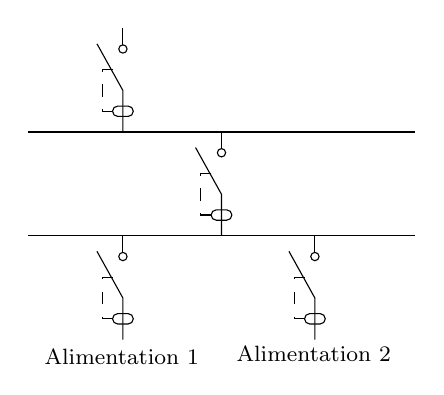
\begin{tikzpicture}[x=0.75pt,y=0.75pt,yscale=-1,xscale=1]
%uncomment if require: \path (0,218); %set diagram left start at 0, and has height of 218

%Straight Lines [id:da9017814347617055] 
\draw    (6.88,65) -- (193.13,65) ;
%Straight Lines [id:da9177255960935432] 
\draw    (40,22.5) -- (52.5,45) -- (52.5,65) ;
%Shape: Circle [id:dp6537007148868619] 
\draw   (54.5,25) .. controls (54.5,23.9) and (53.6,23) .. (52.5,23) .. controls (51.4,23) and (50.5,23.9) .. (50.5,25) .. controls (50.5,26.1) and (51.4,27) .. (52.5,27) .. controls (53.6,27) and (54.5,26.1) .. (54.5,25) -- cycle ;
%Straight Lines [id:da35199593727193423] 
\draw    (52.5,23) -- (52.5,15) ;
%Rounded Rect [id:dp6193458384304921] 
\draw   (47.5,55) .. controls (47.5,53.62) and (48.62,52.5) .. (50,52.5) -- (55,52.5) .. controls (56.38,52.5) and (57.5,53.62) .. (57.5,55) -- (57.5,55) .. controls (57.5,56.38) and (56.38,57.5) .. (55,57.5) -- (50,57.5) .. controls (48.62,57.5) and (47.5,56.38) .. (47.5,55) -- cycle ;
%Straight Lines [id:da9527186101720663] 
\draw  [dash pattern={on 4.5pt off 4.5pt}]  (47.5,35) -- (42.5,35) -- (42.5,55) -- (47.5,55) ;

%Straight Lines [id:da11508322768940726] 
\draw    (87.5,72.5) -- (100,95) -- (100,115) ;
%Shape: Circle [id:dp3391289042502843] 
\draw   (102,75) .. controls (102,73.9) and (101.1,73) .. (100,73) .. controls (98.9,73) and (98,73.9) .. (98,75) .. controls (98,76.1) and (98.9,77) .. (100,77) .. controls (101.1,77) and (102,76.1) .. (102,75) -- cycle ;
%Straight Lines [id:da23522970219666894] 
\draw    (100,73) -- (100,65) ;
%Rounded Rect [id:dp7801124199714764] 
\draw   (95,105) .. controls (95,103.62) and (96.12,102.5) .. (97.5,102.5) -- (102.5,102.5) .. controls (103.88,102.5) and (105,103.62) .. (105,105) -- (105,105) .. controls (105,106.38) and (103.88,107.5) .. (102.5,107.5) -- (97.5,107.5) .. controls (96.12,107.5) and (95,106.38) .. (95,105) -- cycle ;
%Straight Lines [id:da8144885809103521] 
\draw  [dash pattern={on 4.5pt off 4.5pt}]  (95,85) -- (90,85) -- (90,105) -- (95,105) ;

%Straight Lines [id:da5030372720493737] 
\draw    (40,122.5) -- (52.5,145) -- (52.5,165) ;
%Shape: Circle [id:dp6407081872243225] 
\draw   (54.5,125) .. controls (54.5,123.9) and (53.6,123) .. (52.5,123) .. controls (51.4,123) and (50.5,123.9) .. (50.5,125) .. controls (50.5,126.1) and (51.4,127) .. (52.5,127) .. controls (53.6,127) and (54.5,126.1) .. (54.5,125) -- cycle ;
%Straight Lines [id:da6460091175696209] 
\draw    (52.5,123) -- (52.5,115) ;
%Rounded Rect [id:dp9609968233337836] 
\draw   (47.5,155) .. controls (47.5,153.62) and (48.62,152.5) .. (50,152.5) -- (55,152.5) .. controls (56.38,152.5) and (57.5,153.62) .. (57.5,155) -- (57.5,155) .. controls (57.5,156.38) and (56.38,157.5) .. (55,157.5) -- (50,157.5) .. controls (48.62,157.5) and (47.5,156.38) .. (47.5,155) -- cycle ;
%Straight Lines [id:da6179641442257855] 
\draw  [dash pattern={on 4.5pt off 4.5pt}]  (47.5,135) -- (42.5,135) -- (42.5,155) -- (47.5,155) ;

%Straight Lines [id:da00291106623493409] 
\draw    (6.88,115) -- (193.13,115) ;
%Straight Lines [id:da11915371021246435] 
\draw    (132.5,122.5) -- (145,145) -- (145,165) ;
%Shape: Circle [id:dp1952488345903889] 
\draw   (147,125) .. controls (147,123.9) and (146.1,123) .. (145,123) .. controls (143.9,123) and (143,123.9) .. (143,125) .. controls (143,126.1) and (143.9,127) .. (145,127) .. controls (146.1,127) and (147,126.1) .. (147,125) -- cycle ;
%Straight Lines [id:da16332456687050667] 
\draw    (145,123) -- (145,115) ;
%Rounded Rect [id:dp31893341091728067] 
\draw   (140,155) .. controls (140,153.62) and (141.12,152.5) .. (142.5,152.5) -- (147.5,152.5) .. controls (148.88,152.5) and (150,153.62) .. (150,155) -- (150,155) .. controls (150,156.38) and (148.88,157.5) .. (147.5,157.5) -- (142.5,157.5) .. controls (141.12,157.5) and (140,156.38) .. (140,155) -- cycle ;
%Straight Lines [id:da8418511360368651] 
\draw  [dash pattern={on 4.5pt off 4.5pt}]  (140,135) -- (135,135) -- (135,155) -- (140,155) ;


% Text Node
\draw (13.5,168.5) node [anchor=north west][inner sep=0.75pt]   [align=left] {{\footnotesize Alimentation 1}};
% Text Node
\draw (106,167) node [anchor=north west][inner sep=0.75pt]   [align=left] {{\footnotesize Alimentation 2}};
% Text Node
\draw (54.5,30) node [anchor=north west][inner sep=0.75pt]   [align=left] {\cstep\label{pas:40}};
% Text Node
\draw (102,80) node [anchor=north west][inner sep=0.75pt]   [align=left] {\cstep\label{pas:41}};
% Text Node
\draw (147,130) node [anchor=north west][inner sep=0.75pt]   [align=left] {\cstep\label{pas:42}};

\end{tikzpicture}
\subcaption{unifilaire de l'installation}
\end{subfigure}
\begin{subfigure}[b]{0.49\linewidth}
\centering
%--------------------------------------
%ELECTROTECHNIQUE - SCHEMA DE LIAISON A LA TERRE
%--------------------------------------

%utiliser les environnement \begin{comment} \end{comment} pour mettre en commentaire le préambule une fois la programmation appelée dans le document maître (!ne pas oublier de mettre en commentaire \end{document}!)

\begin{comment}

\documentclass[a4paper, 11pt, twoside, fleqn]{memoir}

\usepackage{AOCDTF}

\input{marqueur_chapitre_couleur} %à personnaliser selon le nombre de chapitre dans le cours

%--------------------------------------
%corps du document
%--------------------------------------

\begin{document} %corps du document
	\openleft %début de chapitre à gauche

\end{comment}

\begin{tikzpicture}
\begin{axis}[
/pgf/number format/.cd, use comma, 1000 sep={\,}, %format numérique européen
axis x line=bottom, axis y line = left,
no markers,
width=\linewidth, height=6cm, %hauteur/largeur
legend cell align={left}, legend style={at={(1,1.02)},anchor=south east},
grid=major,
grid=both,
enlarge x limits=false, 
xmode=log, xmin=10, xmax=12000, xtick={10, 100, 1000, 10000},
xlabel style={text width=\linewidth}, ylabel style={text width=5cm},
xlabel={Intensité du courant de fonctionnement résiduels assignés en \si{\milli\ampere}}, log ticks with fixed point,
ymode=log, ymin=10, ymax=13000, ytick={10, 100, 1000, 10000},
ylabel={Durée $t$ du passage du courant en \si{\milli\second}},
]


\path[name path=gbi] (14.517932133997183,10000) -- (14.517932133997183,10) -- (10000,10);
\path[name path=hdi] (29.60932939627084,10000) -- (29.60932939627084,352.7323205216774) -- (146.77992676220705,40.34961693676772) -- (10000,40.34961693676772);
\addplot [blue, opacity=0.5] fill between[of=gbi and hdi];
\addlegendentry{Instantané \Circled{1}};

\path[name path=gbs] (10000,40.34961693676772) -- (2682.6957952797275,40.34961693676772) -- (1973.504382868977,48.54353364246499) -- (704.075200660645,60.39790821830388) -- (289.6708287824031,149.68644761350285) -- (150,502.0302968341689
) -- (150,10000);
\path[name path=hds] (10000,149.68644761350285) -- (1435.9617019622142,149.68644761350285) -- (590.7837911587943,213.04294320497598) -- (590.7837911587943,213.04294320497598) -- (299.357729472049,502.0302968341689
) -- (299.357729472049,10000);
\addplot [red, opacity=0.5] fill between[of=gbs and hds];
\addlegendentry{Sélectif \Circled{2}};

\path[name path=gbr] (10000,150) -- (1655.9515234819182,150) -- (474.45002755086585,502.0302968341689) -- (474.45002755086585,10000);
\path[name path=hdr] (10000,313.5814507256924) -- (4796.808502304898,313.5814507256924) -- (1033.441063880556,919.3982010218539) -- (1033.441063880556,10000);
\addplot  [brown, opacity=0.5]  fill between[of=gbr and hdr];
\addlegendentry{Retardé  \Circled{3}};

\addplot (14.517932133997183,10000) -- (14.517932133997183,10) -- (10000,10) -- (10000,40.34961693676772) -- (146.77992676220705,40.34961693676772) -- (29.60932939627084,352.7323205216774) -- (29.60932939627084,10000) -- cycle;
\addplot [red] (10000,40.34961693676772) -- (2682.6957952797275,40.34961693676772) -- (1973.504382868977,48.54353364246499) -- (704.075200660645,60.39790821830388) -- (289.6708287824031,149.68644761350285) -- (150,502.0302968341689
) -- (150,10000) -- (299.357729472049,10000) -- (299.357729472049,502.0302968341689
) -- (590.7837911587943,213.04294320497598) -- (590.7837911587943,213.04294320497598)  -- (1435.9617019622142,149.68644761350285) -- (10000,149.68644761350285) -- cycle;
\addplot [brown] (10000,150) -- (1655.9515234819182,150) -- (474.45002755086585,502.0302968341689) -- (474.45002755086585,10000) -- (1033.441063880556,10000) -- (1033.441063880556,919.3982010218539) -- (4796.808502304898,313.5814507256924) -- (10000,313.5814507256924) -- cycle;

\end{axis}
\end{tikzpicture}





%\end{document}


\subcaption{courbe des courants de fonctionnement résiduels assignés en fonction du temps\supercite{Schneider:coordinationDDR}}
\end{subfigure}
\end{figure}

\paragraph{Cas particulier de coordination avec les DDR de type B}

\startcstep
\begin{wrapfigure}{R}{0pt}
\ffigbox[\FBwidth]
{\caption{Cas d'une sélectivité à deux niveaux entre des DDR de type B\label{fig:selectivite_DDR_type_B}}}
{\tikzset{every picture/.style={line width=0.75pt}} %set default line width to 0.75pt        

\begin{tikzpicture}[x=0.75pt,y=0.75pt,yscale=-1,xscale=1]
%uncomment if require: \path (0,138); %set diagram left start at 0, and has height of 138

%Straight Lines [id:da8169631390975441] 
\draw    (119.38,65) -- (305.63,65) ;
%Straight Lines [id:da4319979510089893] 
\draw    (152.5,22.5) -- (165,45) -- (165,65) ;
%Shape: Circle [id:dp7461171752369792] 
\draw   (167,25) .. controls (167,23.9) and (166.1,23) .. (165,23) .. controls (163.9,23) and (163,23.9) .. (163,25) .. controls (163,26.1) and (163.9,27) .. (165,27) .. controls (166.1,27) and (167,26.1) .. (167,25) -- cycle ;
%Straight Lines [id:da8451811097550901] 
\draw    (165,23) -- (165,15) ;
%Rounded Rect [id:dp18053555138635746] 
\draw   (160,55) .. controls (160,53.62) and (161.12,52.5) .. (162.5,52.5) -- (167.5,52.5) .. controls (168.88,52.5) and (170,53.62) .. (170,55) -- (170,55) .. controls (170,56.38) and (168.88,57.5) .. (167.5,57.5) -- (162.5,57.5) .. controls (161.12,57.5) and (160,56.38) .. (160,55) -- cycle ;
%Straight Lines [id:da08951652624873063] 
\draw  [dash pattern={on 4.5pt off 4.5pt}]  (160,35) -- (155,35) -- (155,55) -- (160,55) ;

%Straight Lines [id:da7410030620837423] 
\draw    (200,72.5) -- (212.5,95) -- (212.5,115) ;
%Shape: Circle [id:dp05670563209773016] 
\draw   (214.5,75) .. controls (214.5,73.9) and (213.6,73) .. (212.5,73) .. controls (211.4,73) and (210.5,73.9) .. (210.5,75) .. controls (210.5,76.1) and (211.4,77) .. (212.5,77) .. controls (213.6,77) and (214.5,76.1) .. (214.5,75) -- cycle ;
%Straight Lines [id:da816027499463629] 
\draw    (212.5,73) -- (212.5,65) ;
%Rounded Rect [id:dp3947599360896624] 
\draw   (207.5,105) .. controls (207.5,103.62) and (208.62,102.5) .. (210,102.5) -- (215,102.5) .. controls (216.38,102.5) and (217.5,103.62) .. (217.5,105) -- (217.5,105) .. controls (217.5,106.38) and (216.38,107.5) .. (215,107.5) -- (210,107.5) .. controls (208.62,107.5) and (207.5,106.38) .. (207.5,105) -- cycle ;
%Straight Lines [id:da6953851857801584] 
\draw  [dash pattern={on 4.5pt off 4.5pt}]  (207.5,85) -- (202.5,85) -- (202.5,105) -- (207.5,105) ;


% Text Node
\draw (167,30) node [anchor=north west][inner sep=0.75pt]   [align=left] {\cstep\label{pas:50}};
% Text Node
\draw (214.5,80) node [anchor=north west][inner sep=0.75pt]   [align=left] {\cstep\label{pas:51}};
% Text Node
\draw (38.5,4.5) node [anchor=north west][inner sep=0.75pt]  [font=\scriptsize] [align=left] {\begin{minipage}[lt]{76.744375pt}\setlength\topsep{0pt}
\begin{flushright}
DDR\\
type B\\
\SI{300}{\milli\ampere}\\
type S
\end{flushright}

\end{minipage}};
% Text Node
\draw (86,69.5) node [anchor=north west][inner sep=0.75pt]  [font=\scriptsize] [align=left] {\begin{minipage}[lt]{76.744375pt}\setlength\topsep{0pt}
\begin{flushright}
DDR\\
type B\\
\SI{30}{\milli\ampere}
\end{flushright}

\end{minipage}};
\end{tikzpicture}}
\end{wrapfigure}

En présence d'un courant de fuite à la terre possible en courant continu (typiquement le cas pour les chargeurs de voiture), un DDR de type B doit être utilisé pour la protection contre les contacts indirects. Dans ce cas, le DDR en amont ne doit pas être aveuglé par le courant résiduel continu possible et doit assurer sa protection normale lorsqu'un courant de défaut apparait dans une autre partie de l'installation.\\
Par exemple, dans le schéma en \superref{fig:selectivite_DDR_type_B}, le DDR $I_{\Delta n} = \SI{30}{\milli\ampere}$ de type B au niveau 2 peut avoir un seuil de déclenchement courant continu maximum de $2 \times I_{\Delta n}$, selon la norme produit DDR CEI 62423\supercite{IEC:62423-2009}. Cela signifie que ce DDR de $I_{\Delta n} = \SI{30}{\milli\ampere}$ de type B pourrait laisser passer un courant résiduel de presque \SI{60}{\milli\ampere} $\mathdirectcurrent$ sans déclenchement et que le DDR en amont ne devrait perdre aucune de ses performances avec la présence de ce niveau élevé de courant résiduel $mathdirectcurrent$. C'est pourquoi il est souvent proposé d'utiliser un DDR de type B au niveau 1 pour éviter tout effet d'aveuglement par le courant continu.\\

Toutefois, certains constructeurs implémentent dans leurs DDR de type A la capacité de ne pas être sensibles au courant résiduel $\mathdirectcurrent$ en dessous d'un certain seuil de courant de défaut ($\SI{60}{\milli\ampere}$ pour la marque Schneider\supercite{Schneider:coordinationDDR}. Cela permet d'éviter la pose d'un DDR de type B en amont, plus coûteux qu'un DDR de type A, tout en conservant les capacités de détection des DDR de types A et AC.

\subsection{Mise à la terre des appareils et structures conductrices}

\subsubsection{Mise à la terre des appareils électriques}

Les appareils de classe d'isolation I doivent être raccordées à des prises 2P + T \circrefseul{pas:30} au moyen de fiches 2P + T \circrefseul{pas:31}. Ces prises équipent maintenant tous les logements dont l'installation respecte la norme NF C15-100. Si ces appareils ne présentent pas de fiches, elles sont raccordées au moyen de boitiers d'encastrements appropriés.\\
Sont particulièrement concernés par cette connexion vers la terre les appareils combinant électricité et eau (lave-vaisselle, lave-linge, cafetière\ldots \circrefseul{pas:32}). Les fuites d'eau peuvent effectivement  provoquer relativement facilement la mise sous tension de la carcasse métallique de l'appareil.

\subsubsection{Liaison équipotentielle}

Pour protéger les biens et les personnes des contacts indirects, en plus de connecter toutes les carcasses métalliques des appareils de classe d'isolation II vers la terre, il convient de connecter toutes les structures métalliques du bâtiment susceptibles d'être en contact avec un individu \emph{et} d'être mise sous tension accidentellement. Sont concernés par la mise à la terre \circrefseul{pas:33} :
\begin{itemize}
\item tuyauterie (même non conductrice car l'eau y transitant l'est)\,;
\item baignoire et bac de douche (fonte, métal\ldots)\,;
\item charpente métallique\,;
\item autres structures métalliques (pouvant varier selon les exigences de sécurité).
\end{itemize}
Cette connexion, effectuée par un \emph{conducteur de protection} PE \circrefseul{pas:34} (obligatoirement en jaune-vert), de toutes les structures conductrices et appareils de classe I constitue la \emph{liaison équipotentielle}. Tous ces conducteurs sont connectés sur une \emph{barrette de terre} \circrefseul{pas:37} dans le Tableau Général Basse Tension (TGBT) et sont séparés de la \emph{prise de terre de l'installation électrique} \circrefseul{pas:38} par une \emph{barrette de mesure} \circrefseul{pas:39} (dénommé également \emph{couteau de terre}).\\

Afin d'assurer la meilleure protection possible, les conducteurs de protection doivent présenter une section de câble et des raccordements dimensionnés à même de garantir une résistance de la liaison équipotentielle d'une valeur inférieure à \SI{2}{\ohm}. Cette résistance est contrôlée au moyen d'un \emph{testeur de continuité} spécifique.
\begin{table}[H]
\caption{Section des conducteurs de protection}
\begin{tabularx}{\linewidth}{c X p{5,5cm}}
\toprule
\thead{Schéma}		& \thead{Type de conducteur}		& \thead{Section} \\
\midrule
\circrefseul{pas:34} 		& Conducteur de protection transitant dans la même canalisation que les phase(s) et neutre		& identique à celle des phase(s) et neutre \\
\addlinespace
	&		Conducteur de protection protégé mécaniquement																	& \SI{2,5}{\square\milli\meter} \\
\addlinespace
	&		Conducteur de protection non protégé mécaniquement															& \SI{4}{\square\milli\meter} \\
\addlinespace
\circrefseul{pas:35}		&	Conducteur principal de protection																							& \SI{16}{\square\milli\meter} en cuivre isolé \\
\addlinespace
\circrefseul{pas:36} 		& Conducteur de terre																												& 
\begin{tabdescription}
\item[Selon les caractéristiques :]\hfill
\begin{compactitemize}
\item \SI{16}{\square\milli\meter} en cuivre isolé\,;
\item \SI{25}{\square\milli\meter} en cuivre nu\,;
\item \SI{50}{\square\milli\meter} en aluminium ou en fer.
\end{compactitemize} 
\end{tabdescription}
\\
\bottomrule
\end{tabularx}
\end{table}

\input{fig_equipotentielle}

\subsubsection{Prise de terre de l'installation électrique\label{subsec:prise_terre_installation_electrique}}

Le courant de défaut $I_d$ transite par les conducteurs de la liaison équipotentielle et s'échappe vers la terre via la \emph{prise de terre de l'installation électrique} \circrefseul{pas:38} qui est simplement un électrode métallique en contact avec la terre.\\
Cet électrode doit présenter également la plus faible \emph{résistance de terre} $R_A$ pour permettre au courant de défaut $I_d$ de s'échapper sous une \emph{tension de sécurité} $U_L$ la plus faible possible.  Cette valeur doit être régulièrement contrôlée par un \emph{contrôleur de terre}. Les paramètres $U_L$ et $I_{\Delta n}$ (calibre du DDR) étant des constantes déterminées par le DDR, le seul paramètre variable est donc la $R_A$, selon les conditions environnementales (géologie, humidité, corrosion\ldots).\\
Elle ne doit jamais dépasser :
\begin{description}
\item[\SI{50}{\ohm} :] locaux humides\,;
\item[\SI{100}{\ohm} :] locaux secs.
\end{description}

\begin{formule}[Valeur de la résistance de la prise de terre de l'installation électrique $R_T$\label{form:resistance_prise_terre}]
\begin{align}
R_A &\leq \frac{U_L}{I_{\Delta n}}
\end{align}
\end{formule}

\begin{textvariables}
R_A			& résistance		& ohm		& \ohm 		& résistance de la prise de terre \\
U_L			& tension			& volt		& \volt		& tension de sécurité du local \\
I_{\Delta n}	& intensité			& ampère	& \ampere	& intensité de sensibilité du DDR (calibre) \\
\end{textvariables}

Il existe trois méthode de mesure de $R_A$ :
\begin{description}
\item[mesure en ligne (des 62\%) :] un ou deux piquets selon les variantes\,;
\item[mesure en triangle :] deux piquets disposés de façon à former un triangle équilatéral avec le piquet de terre.
\end{description}

La terre est un conducteur offrant une résistance bien plus élevée que le cuivre mais sa \og section \fg{} est théoriquement infinie, on va donc maximiser la surface de contact de la prise de terre de l'installation électrique. Il existe trois technique courant pour la réaliser :

\paragraph{Boucle à fond de fouille}
Cette technique consiste en un conducteur noyé dans les fondations et raccordée à la boucle. Elle est réalisée lors du terrassement précédant la construction de l'immeuble et constitue la solution privilégiée pour minimiser la résistance de terre $R_A$. Elle sera donc préférée aux deux solutions suivantes.\\
Le conducteur utilisé doit cependant présenter une section minimale selon le matériau choisi :
\begin{itemize}
\item câble de cuivre nu de \SI{25}{\square\milli\meter}\,;
\item câble en acier de \SI{95}{\square\milli\meter}\,;
\item feuillard en acier de \SI{100}{\square\milli\meter} et de \SI{3}{\milli\meter} d'épaisseur.
\end{itemize}
\input{fig_boucle_terre}

\paragraph{Câble en tranchée}
Si la mise en \oe{}uvre de la boucle à fond de fouille n'est pas possible (bâtiment existant par exemple), on peut réaliser la mise à la terre de l'installation électrique par l'installation d'un câble en tranchée en respectant les règles de pose explicité dans le schéma \superref{fig:cable_tranchee}.\\
Le conducteur utilisé doit aussi présenter une section minimale selon le matériau choisi :
\begin{itemize}
\item câble de cuivre nu de \SI{25}{\square\milli\meter}\,;
\item câble en acier de \SI{95}{\square\milli\meter}.
\end{itemize}

\input{fig_cable_tranchee}

\paragraph{Piquet de terre}
Si aucune des deux solutions précédentes n'est envisageable, on peut réaliser la prise de terre au moyen d'un piquet enfoncé dans le sol en respectant les règles de pose explicité dans le schéma \superref{fig:piquet_terre}.\\
Le piquet utilisé doit aussi présenter une section ou une surface minimale selon le matériau choisi :
\begin{itemize}
\item tube en acier de \SI{25}{\milli\meter} de diamètre\,;
\item profilé en acier de \SI{60}{\square\milli\meter} de diamètre\,;
\item une barre de cuivre ou d'acier cuivré de \SI{15}{\square\milli\meter} de diamètre.
\end{itemize}

\input{fig_piquet_terre}

\subsection{Mise hors de portée des appareils électriques}

Un dernier moyen de protection contre les contacts indirects est de mettre hors de portée les appareils électriques ou du moins installer des appareils présentant des indices de protections adaptés à l'environnement. Cette solution est obligatoirement appliquée dans les pièces humides comme les salles de bain ou de douches, et les règles d'installations sont régies par la norme NF-C15 100\supercite{NF:C15-100-2015}.\\
L'eau étant conductrice, si l'on se retrouve immergé ou simplement mouillé, le risque d'électrocution lors de la manipulation d'appareils est plus important. Les zones humides font donc l'objet d'une attention particulière :
\begin{itemize}
\item règlementation de pose des appareils électrique\,;
\item calibre du DDR plus faible ($I_{\Delta n}<\SI{30}{\milli\ampere}$)\,;
\item liaison équipotentielle \emph{secondaire} (huisseries, tuyauterie, baignoire métallique, plancher chauffant, crépine\ldots).
\end{itemize}

\input{fig_volume_douche}
\input{fig_volume_bain}

\begin{table}[t]
\caption{Caractéristiques des équipements électriques selon les volumes des salles d'eau}
\begin{threeparttable} %note dans tableau
\begin{tabularx}{\linewidth}{X ccccc}
\toprule
\multirow[c]{2}{*}{\thead{Appareils}} 	& \multirow[c]{2}{*}{\thead{Mesure de\\protection}}		& \thead{Volume 0}		& \thead{Volume 1}		& \thead{Volume 2}		& \multirow{2}{*}{\thead{Hors volume}} \\
&&	IPX7		& IPX4\tnote{1}			& IPX4\tnote{1}			& \\
\midrule
Lave-linge, sèche-linge				& classe I													& interdit						& interdit 						& interdit						& autorisé \\
\addlinespace
Appareils de chauffage 				& classe I												& interdit						& interdit 						& interdit						& autorisé \\
												&classe II												& interdit						& interdit 						& autorisé						& autorisé \\
\addlinespace
\'Eclairage									& classe I													& interdit						& interdit 						& interdit						& autorisé \\
												& classe II													& interdit						& interdit 						& autorisé						& autorisé \\
												& \adjustbox{valign=t}{\makecell[{{p{2,5cm}}}]{TBTS (\SI{12}{\volt} $\mathdirectcurrent$ ou \SI{30}{\volt} $\sim$)}}												& autorisé\tnote{2}						& autorisé\tnote{2} 						& autorisé\tnote{2}						& autorisé\tnote{3} \\
\addlinespace
Chauffe-eau instantané				& classe I													& interdit						& autorisé\tnote{4} 					& autorisé\tnote{4}						& autorisé \\
\addlinespace
Chauffe-eau à accumulation				& classe I												& interdit						& autorisé\tnote{5} 					& autorisé\tnote{4}						& autorisé \\
\addlinespace
Interrupteur								& 																& interdit						& interdit 						& interdit						& autorisé \\
												& \adjustbox{valign=t}{\makecell[{{p{2,5cm}}}]{TBTS (\SI{12}{\volt} $\mathdirectcurrent$ ou \SI{30}{\volt} $\sim$)}}	& interdit						& autorisé\tnote{2} 						& autorisé\tnote{2}						& autorisé\tnote{3} \\
\addlinespace
Prise de courant avec terre			& 																& interdit						& interdit 						& interdit						& autorisé \\
\addlinespace
Prise rasoir (\SIrange{10}{50}{\watt})								& \adjustbox{valign=t}{\makecell[{{p{2,5cm}}}]{transformateur de séparation}}															& interdit						& interdit 						& autorisé						& autorisé \\
\addlinespace
Transformateur de séparation							& 															& interdit						& interdit 						& interdit						& autorisé \\
\addlinespace
Canalisation							& 															& interdit						& autorisé\tnote{6} 						& autorisé\tnote{6}						& autorisé \\
\addlinespace
Boitier de connexion							& 															& interdit						& interdit\tnote{7} 						& interdit						& autorisé \\
\bottomrule
\end{tabularx}
\begin{tablenotes}
    \item[1] IP X5 si le volume est soumis à des jets d'eau pour des raisons de nettoyage (piscines, bains publics\ldots)\,;
    \item[2] Le transformateur de séparation doit être installé en dehors des volumes 1, 2 et 3\,;
	\item[3] La tension peut être portée à \SI{230}{\volt}\,;
	\item[4] Si l'appareil est alimenté directement sans boite de connexion\,;
	\item[5] Chauffe-eau horizontal installé le plus haut possible\,;
	\item[6] Limité à l'alimentation des appareils autorisés dans ces volumes\,;
	\item[7] Pour l'alimentation en direct d'un appareil et avec le respect de l'IP exigée par le volume ou elle se situe.
\end{tablenotes}
\end{threeparttable} %note dans tableau
\end{table}


%\end{document}


%--------------------------------------
%conclusion, bibliographie
%--------------------------------------

\backmatter

	%--------------------------------------
	%inclusion des chapitres
	%--------------------------------------


	%--------------------------------------
	%bibliographie
	%--------------------------------------

	\nocite{AFPA2000, BourgeoisCogniel2005, CNED:SLT2003, Juguet2017, Hager:manueltechnique, Legrand:pointsclesNFC15-100, LyceeJean-Caillaud:PRE2013, NF:C15-100-2015, Schneider:DDR, Schneider:SLT, WildiSybille2014}
	
	\printbibliography %ajout des références bibliographiques
		
\end{document}

